% Entwurf der Doktorarbeit von Domenik Zimmermann, TU M\"unchen, Grp. Prof. Dr. Auw\"arter 
%%%%%%%%%%%%%%%%%%%%%%%%%%%%%%%%%%%%%%%%%%%%%%%%%%%%%%%
\author{Domenik Matthias Zimmermann}
\title{Molecular fictionalization of h-BN}
%%%%%%%%%%%%%%%%%%%%%%%%%%%%%%%%%%%%%%%%%%%%%%%%%%%%%%%
% Bilder: AFM/STM 1024x1024 px exportieren, 
%
% Fonts are embedded by default, otherwise check 
% https://tex.stackexchange.com/questions/10391/how-to-embed-fonts-at-compile-time-with-pdflatex
% 
% sudo apt-get install kile texlive-latex-extra texlive-science texlive-bibtex-extra biber
% adjust kile tools to call biber %lS instead of bibtex
%
% If errors occure referring to aux files or others:
%	Delete helper files (*.aux) and maybe others!
%
% Use MikTeX version 2.9.6615 or later (check that biber is included)
% Using BiBLaTex, biber as frontend.
% If biber complains (ERROR - Error: Found biblatex control file version 2.6, expected version 3.4.)
% 	Update with your Miktex package manager (mpm_mfc.exe[single user install] or mpm_mfc_admin.exe [all user install])
% no new biblatex version there? Sync database? NO omprovement!
%%%%%%%%%%%%%%%%%%%%%%%%%%%%%%%%%%%%%%%%%%%%%%%%%%%%%%%%%%%%%%%%%%%%%%%%%%%%%%%%%%
\documentclass[10pt,a4paper,twoside
,BCOR=8mm				% Bindekorrektur inkl. Biegefalz
,headings=normal		% Kleinere Kapitelüberschriften => check preamble
,headsepline			% Enable line to seperate head ...
,footsepline			% ... and foot
,plainfootsepline		% Footseperation line on chapter start
]{scrbook}
%%%%%%%%%%%%%%%%%%%%%%%%%%%%%%%%%%%%%%%%%%%%%%%%%%%%%%%%%%%%%%%%%%%%%%%%%%%%%%%%%%
%%%%%%%%%%%%%%%%%%%%%%%%%%%%%%%%%%%%%%%%%%%%%%%%%%%%%%%%%%%%%%%%%%%%%%%%%%%%%%%%%%
\usepackage[utf8]{inputenc}
% when latex complains about unicode char U+2212 is not configured for use in latex use the line below
\DeclareUnicodeCharacter{2212}{-}% support older LaTeX versions
%\usepackage[latin1]{inputenc}
\usepackage[T1]{fontenc}
\usepackage{lmodern}
\usepackage[english]{babel}
\usepackage{csquotes}
\usepackage{amsmath}
\usepackage{textcomp}		%enables \textdegree to use as �
\usepackage{amsfonts}
\usepackage{amssymb}
\usepackage{graphicx}
\usepackage{xhfill}			% provides /hrulefill (disclaimer)
%\usepackage{wasysym}		
\usepackage{braket}		% fur <A|H|B> <A| |A> oder <A>
%\DeclareGraphicsExtensions{.pdf,.png,.jpg}
%%%%%%%%%%%%%%%%%%%%%%%%%%%%%
\usepackage{siunitx}
\DeclareSIUnit\langmuir{L}
%%%%%%%%%%%%%%%%%%%%%%%%%%%%%
\usepackage[hidelinks,breaklinks=true]{hyperref}
%\usepackage{url}
\usepackage[section]{placeins} %definiert \floatbarrier, mit option automatisch bei jeder section
%%%%%%%%%%%%%%%%%%%%%%%%%%%%%%%%%%%%%%%%%%%
\usepackage{subfigure}
\usepackage{wrapfig}
%%%%%%%%%%%%%%%%%%%%%%%%%%%%%%%%%%%%%%%%%%%
\usepackage{caption}
\usepackage{microtype}
%\usepackage{subcaption}
\usepackage{multicol}
\usepackage{multirow}
%%%%%%%%%%%%%%%%%%%%%%%%%%%%
% fuer Stichwortverzeichnis
\usepackage{makeidx}
% Stichwortverzeichnis erstellen
\makeindex
%%%%%%%%%%%%%%%%%%%%%%%%%%%%%%%%%%%%%%%%%%%%%%%%%%%%%%%
\usepackage[style=numeric		% bibliogryphy-styles: alphabetic, numeric, chem-angew, ieee, nature, science
,backend=biber
%,refsection=chapter			% setzt bibliographies nach chaptern getrennt, nach jedem chapter muss ein 
								% printbibliogrphy stehen
]{biblatex} 	
\addbibresource{./bib.bib}  	% relative to root directory (where the file that includes this file is located)! 
								%do NOT OMIT .bib ending

%avoids ugly line breaks within bibligraphy
\addto\bibsetup{\setlength{\emergencystretch}{1.5em}} 	

% Zum Verwalten der Zitate benutze ich Zotero, zum Erzeugen der .bib-Datein f�r Latex wird die Exportfunktion von Zotero benutzt (rechtsklick auf ``Meine Bibliothek'' im linken Reiter: Option Biblatex in die Datei bib-zotero-export.bib aus welcher ich dann die betreffenden Zitate auf Richtigkeit \"uberpr\"ufe und in die bib.bib kopiere.
%%%%%%%%%%%%%%%%%%%%%%%%%%%%%%%%%%%%%%%%%%%%%%%%%%%%%%%
% \usepackage[top=2.5cm,left=2.5cm,right=3.5cm,bottom=3.5cm]{geometry}
%%%%%%%%%%%%%%%%%%%%%%%%%%%%%%%%%%%%%%%%%%%%%%%%%%%%%%%
\usepackage{xcolor}
%%%%%%%%%%%%%%%%%%%%%%%%%%%%%%%%%%%%%%%%%%%%%%%%%%%%%%
%%%%%%%%%%%%%%%%%%%%%%%%%%%%%%%%%%%%%%%%%%%%%%%%%%%%%%
\usepackage[draft=false]{scrlayer-scrpage}		%deaktiviert ruler in der draft version
\pagestyle{scrheadings}
%%%%%%%%%%%%%%%%%%%%%%%%%%%%%%%%%%%%%%%%%%%%%%%%%%%%%%
%%%%%%%%%%%%%%%%% DAUMENKINO Footer %%%%%%%%%%%%%%%%%%
	\usepackage{etex}
	\usepackage{intcalc} 
	\newcommand*{\AnzBilder}{200}		            		%<--Variablen anpassen
\newcommand*{\KinoPfad}{./images/animation/lumo/} 	%<--Variablen anpassen

%%%%Quelltext%%%
\newcommand*{\SafeboxName}{sbKino}

\makeatletter
%Erzeugt neue Saveboxen und füllt sie mit includegraphics-Anweisungen
%Aufruf: \NewSaveBoxes{sbKino}{5}{daumenkino/kino}
\newcommand*{\NewSaveBoxes}[3]{%
	\@tempcnta 1
	\@whilenum \@tempcnta< \numexpr(#2+1) \do{%
		%Savebox anlegen
		\expandafter\newsavebox\csname #1\the\@tempcnta\endcsname
		%Savebox mit Leben füllen
		\expandafter\savebox\csname #1\the\@tempcnta\endcsname{%
			\includegraphics[width=0.5cm]{#3\the\@tempcnta}%
		}%
		\advance\@tempcnta 1
	}%
}

\newcommand*{\bildnr}{\numexpr\intcalcMod{\numexpr\value{page}}{\numexpr\AnzBilder}\relax}
\newcommand*{\lumoseries}{%
	\usebox{\@nameuse{\SafeboxName\the\bildnr}}%
}
\makeatother
\NewSaveBoxes{\SafeboxName}{\AnzBilder}{\KinoPfad}
	%inner side of odd pages
	\lofoot[\lumoseries]{\lumoseries} % Add flicker books to [plain.scrheadins] and {scrheadins}!
	% inner side of even pages	
	\newcommand*{\AnzBilderLogo}{200}		            		%<--Variablen anpassen
\newcommand*{\KinoPfadLogo}{./images/animation/logo/} 	%<--Variablen anpassen
%%%%Quelltext%%%
\newcommand*{\SafeboxNameLogo}{sbKinologo}

\makeatletter
%Erzeugt neue Saveboxen und füllt sie mit includegraphics-Anweisungen
%Aufruf: \NewSaveBoxesLogo{sbKino}{5}{daumenkino/kino}
\newcommand*{\NewSaveBoxesLogo}[3]{%
	\@tempcntb 1
	\@whilenum \@tempcntb< \numexpr(#2+1) \do{%
		%Savebox anlegen
		\expandafter\newsavebox\csname #1\the\@tempcntb\endcsname
		%Savebox mit Leben füllen
		\expandafter\savebox\csname #1\the\@tempcntb\endcsname{%
			\includegraphics[width=0.5cm]{#3\the\@tempcntb}%
		}%
		\advance\@tempcntb 1
	}%
}
%intcalc-version
\newcommand*{\bildnrLogo}{\numexpr\intcalcMod{\numexpr\value{page}}{\numexpr\AnzBilderLogo}\relax}

\newcommand*{\logoseries}{%
	\usebox{\@nameuse{\SafeboxNameLogo\the\bildnrLogo}}%
}
\makeatother
\NewSaveBoxesLogo{\SafeboxNameLogo}{\AnzBilderLogo}{\KinoPfadLogo}
%%%Aufruf%%%%%%%
	\refoot[\logoseries]{\logoseries} % Add flicker books to [plain.scrheadins] and {scrheadins}!
%%%%%%%%%%%%%%%%%%%%%%%%%%%%%%%%%%%%%%%%%%%%%%%%%%%%%%
%%%%%%%%%%%%%%%%%%%%%%%%%%%%%%%%%%%%%%%%%%%%%%%%%%%%%%
% Basic information for cover & title page
\newcommand*{\getUniversity}{Technische Universit\"at M\"unchen}
\newcommand*{\getFaculty}{Department of physics}
\newcommand*{\getFacultyger}{Fakult\"at f\"ur Physik}
\newcommand*{\getTitle}{Molecular adsorption on \textit{h}-BN}
%newcommand*{\getTitleger}{TODO: Titel der Abschlussarbeit}
\newcommand*{\getAuthor}{Domenik Matthias Zimmermann}
\newcommand*{\getDoctype}{Dissertation}
\newcommand*{\getDoctypeger}{Vollst\"andiger Abdruck der von der Fakult\"at für Physik der Technischen Universit\"at M\"unchen zur Erlangung des akademischen Grades eines Doktors der Naturwissenschaften (Dr. rer. nat.) genehmigten Dissertation.}
\newcommand*{\getSupervisor}{Prof.\ Dr.\ Wilhelm Auw\"arter}
\newcommand*{\getChairman}{TODO: Chairman}
\newcommand*{\getFirstExaminer}{TODO: 1. Examiner}
\newcommand*{\getSecondExaminer}{TODO: 2. Examiner}
\newcommand*{\getSubmissionDate}{TODO: Submission date}
\newcommand*{\getSubmissionLocation}{Munich}
\newcommand*{\getDisclaimer}{I assure the single handed composition of this \MakeLowercase{\getDoctype{}} only supported by declared resources.}
% TODO: add custom commands etc.

%%%%%%%%%%%%%%%%%%%%%%%%%%%%%%%%%%%%%%%%%%%%%%%%%%%%%%%%%%%%%%%%%%%%%%%%%%%%%%%%%%%%%%%%%%%%%
% Change \autoref (Figure x.x) to FIGURE x.x

%%%%%%%%%%%%%%%%%%%%%%%%%%%%%%%%%%%%%%%%%%%%%%%%%%%%%%%%%%%%%%%%%%%%%%%%%%%%%%%%%%%%%%%%%%%%%
% Python style for highlighting
% Check https://tex.stackexchange.com/questions/83882/how-to-highlight-python-syntax-in-latex-listings-lstinputlistings-command#83883

% Default fixed font does not support bold face
\DeclareFixedFont{\ttb}{T1}{txtt}{bx}{n}{12} % for bold
\DeclareFixedFont{\ttm}{T1}{txtt}{m}{n}{12}  % for normal

\newcommand\pythonstyle{\lstset{
		language=Python,
		basicstyle=\small,             %\ttm, \tiny \small
		otherkeywords={self},             % Add keywords here
		keywordstyle=\small\color{deepblue},
		emph={MyClass,__init__},          % Custom highlighting
		emphstyle=\small\color{deepred},    % Custom highlighting style
		stringstyle=\color{deepgreen},
		frame=tb,                         % Any extra options here
		showstringspaces=false,           % 
		frame=single,
		numbers = left,
		numbersep=5pt
}}
% Python environment
\lstnewenvironment{python}[1][]
{
	\pythonstyle
	\lstset{#1}
}
{}
% Python for external files
\newcommand\pythonexternal[2][]{{
		\pythonstyle
		\lstinputlisting[#1]{#2}}}
% Python for inline
\newcommand\pythoninline[1]{{\pythonstyle\lstinline!#1!}}
%%%%%%%%%%%%%%%%%%%%%%%%%%%%%%%%%%%%%%%%%%%%%%%%%%%%%%%%%%%%%%%%%%%%%%%%%%%%%%%%%%%%%%%%%%%%%

%%%%%%%%%%%%%%%%%%%% Draft Mode Compilation from command line %%%%%%%%%%%%%%%%%%%%
%%%%%%%%%%%%%%%%%%%% pdflatex "\def\draftmode{1} \input{FILE}"  %%%%%%%%%%%%%%%%%%
%%%%%% TEXSTUDIO %%% pdflatex "\def\draftmode{1} \input{%.tex}" %%%%%%%%%%%%%%%%%%
%%%%%%%%%%%%%%%%%%%%%%%%%%%%%%%%%%%%%%%%%%%%%%%%%%%%%%%%%%%%%%%%%%%%%%%%%%%%%%%%%%
%\def\daumenkino{1}
%%%%%%%%%%%%%%%%%%%%%%%%%%%%%%%%%%%%%%%%%%%%%%%%%%%%%%%%%%%%%%%%%%%%%%%%%%%%%%%%%%
%%%%%%%%%%%%%%%%%%%%%%%%%%%%%%%%%%%%%%%%%%%%%%%%%%%%%%%%%%%%%%%%%%%%%%%%%%%%%%%%%%
%%%%%%%%%%%%%%%%%%%%%%%%%%%%%%%%%%%%%%%%%%%%%%%%%%%%%%%%%%%%%%%%%%%%%%%%%%%%%%%%%%
%%%%%%%%%%%%%%%%%%%%%%%%%%%%%%%%%%%%%%%%%%%%%%%%%%%%%%%%%%%%%%%%%%%%%%%%%%%%%%%%%%
\begin{document}
%%%%%%%%%%%%%%%%%%%%%%%%%%%%%%%%%%%%%%%%%%%%%%%%%%%%%%%%%%%%%%%%%%%%%%%%%%%%%%%%%%%%%%%%%%%%%%%%%%%%%
 \begin{titlepage}
% HACK for two-sided documents: ignore binding correction for cover page.
% Adapted from Markus Kohm's KOMA-Script titlepage=firstiscover handling.
% See http://mirrors.ctan.org/macros/latex/contrib/koma-script/scrkernel-title.dtx,
% \maketitle macro.
\oddsidemargin=\evensidemargin\relax
\textwidth=\dimexpr\paperwidth-2\evensidemargin-2in\relax
\hsize=\textwidth\relax
%%
\centering
\vspace{50mm}

\includegraphics[width=40mm]{./includes/logo/tum} \\
\vspace{10mm}
{\Huge\MakeUppercase{\getUniversity{}}} \\
\vspace{15mm}
{\huge\MakeUppercase{\getFaculty{}}} \\
\vspace{20mm}
{\Large \getDoctype{}} \\
\vspace{15mm}
{\huge\bfseries \getTitle{}} \\
\vspace{15mm}
{\LARGE \getAuthor{}} \\
\vspace{20mm}

\includegraphics[width=20mm]{./includes/logo/physics}
\end{titlepage}											%					%
 \frontmatter{}			 														%					%
   \begin{titlepage}
\begin{center}
\centering
\vspace{50mm}

\includegraphics[width=40mm]{./includes/logo/tum} \\
\vspace{10mm}
{\Huge\MakeUppercase{\getUniversity{}}} \\
\vspace{15mm}
{\huge\MakeUppercase{\getFaculty{}}} \\
\vspace{20mm}
{\Large \getDoctype{}} \\
\vspace{15mm}
{\huge\bfseries \getTitle{}} \\
\vspace{15mm}
\end{center}
\getDoctypeger{} \\
\vspace{15mm}
%{\huge\bfseries \getTitle{}} \\
%\vspace{10mm}

\begin{center}
\begin{tabular}{l l}
Author: & \getAuthor{} \\
Supervisor: & \getSupervisor{} \\
Submission Date: & \getSubmissionDate{} \\ \hline
Chairman: & \getChairman{} \\
1. Examiner: & \getFirstExaminer{} \\
2. Examiner: & \getSecondExaminer{} \\
\end{tabular}
%\vspace{10mm} \\
%
\includegraphics[width=20mm]{./includes/logo/physics}
\end{center}
\end{titlepage}										%					%
   \thispagestyle{empty}
\vspace*{0.75\textheight}
\noindent
\getDisclaimer{}
\vskip8ex \noindent \hrulefill\par  
\noindent \getSubmissionLocation{}, \getSubmissionDate{} \hspace{2cm} \getAuthor{}
\cleardoublepage{}									% 					%
   \addcontentsline{toc}{chapter}{Acknowledgments}		%Entry in TOC
\thispagestyle{empty}
%\vspace*{2cm}
\begin{center}
{\usekomafont{section} Acknowledgments}
\end{center}
\vspace{1cm}
A lot of people are invoked in the course of the thesis and I like to thank them for their support. First and foremost I like to thank Prof.\ Dr.\ W.\ Auw\"arter for the opportunity to work in his research group. The wide field of molecular assembly and functionalization opened up many interesting insights that would never be possible without him. The time dedicated to experiments under his leadership was very exciting and his review challenged my ambition to further improve. Together with Prof.\ Dr.\ J.\ Barth a very pleasant professional environment was created with retreats and group activities framing our day-to-day work.

Besides them, many people were incorporated at different levels, starting from introducing technical aspects and measurement techniques used at the different setups via result discussion through to proof-reading and concept validation. 

	Dr.\ A.\ Wiengarten was the operator of the low temperature scanning tunneling microscope and I started under her supervision with the first measurements. Her profound understanding of the setup shared with me was consolidated by Dr.\ K.\ Seufert whose deep commitment nurtured my engagement. His enjoyment of work eased many hours in the lab.

	Measurements at the low temperature atomic force microscope are supported by M.\ P\"ortner and S.\ Synkule. Their fruitful result discussion together with Dr.\ A.\ Riss clarified topics in technical and scientific aspects easily.

	The combined room temperature STM and X-Ray photoelectron spectroscopy setup was assembled by Dr.\ M.\ Schwarz whose continuous efforts in setup details enabled the use of this machine. Together with discussion and operational help of A.\ Baklanov, many measurements were done smoothly.

	Further XPS measurements were done at the machine operated by the Nanosystems Initiative Munich represented by \textbf{\underline{LALALA}} and advocated by Dr.\ J.\ Reichert. Scientific discussion with him, K.\ Eberle and Prof.\ Dr.\ Feulner often lead to meaningful outcomes and was always a pleasure.

	The few measurements at the scanning electron microscope were done under supervision of Dr.\ \textbf{\underline{LALALA}} and Y.\ Gong.

	Please let me thank all member of E20 for a nice time together that showed me the value of social interaction combined with consuming delights and limits.

\begin{center}Thank you.
\newpage 
\thispagestyle{empty}
Dedicated to the beloved ones that made me who I am. Without you these endless lines of text would never end. 
%\epigraph{All work and no play makes Jack a dull boy}{James Howell\\Paroimiographia}
%\epigraph{Goodbye, Jake. I love you, dear.}{Stephen King, The Dark Tower} 
\epigraph{Gone. Like a candle-flame. To whatever worlds there are.}{Stephen King, The Dark Tower}
\epigraph{We go to seek a better world. May you find one, as well.}{Stephen King, The Dark Tower}
\end{center}
\cleardoublepage{}								%	 				%
   \chapter{\abstractname}
Good quality, two dimensional, hexagonal boron nitride (\textit{h}-BN) islands require a clean and flat surface to grow on. Techniques to chemically polish the surface are shortly reviewed. After polish the growth of sub-monolayer \textit{h}-BN islands is investigated on poly crystalline copper surfaces by means of STM and XPS. The use of \textit{h}-BN grown on polycrystalline copper foils as insulating and electronically decoupling substrate is shown by reproducing molecular adsorption known on \textit{h}-BN grown on single crystalline copper.

Different molecular species are investigated with regard to their electronic properties and structures formed by self-assembly on metallic and insulating 2D \textit{h}-BN substrates.

Bis- \& Tetra-pyridin-4-ylethynyl functionalized pyrene molcules are adsorped on \textit{h}-BN/Cu(111) to show the diversity of self-assembled molecules structures that can be steered by the number and position of functional groups. It is shown that their opto-electronic properties and assembly after adsorption are well determined by the chemical design of the molecule and show the same trend as gas-phase calculations: An decrease in electronic band gap with increasing number of functional groups. Frontier orbital resolution in STM with modified tip conditions and a wide band gap in STS show efficient decoupling from the metallic substrate by the \textit{h}-BN layer. It modifies the substrate surface potential, so that the band gap is changed locally in a well defined, periodic manner, following the periodicity of \textit{h}-BN's superstructure on Cu(111).

Furthermore coronene molecules are used to determine the influence of a BN modified molecular center on the self-assembly and electronic structure on Ag(111) and Au(111) substrates and shows the importance of the side groups in the formation process of self-assembled structures. Investigation with nc-AFM is used to clarify sub-molecular structure and the formation of linked structures after annealing treatment in UHV.

Single and bis- nitro functionalized porphine molecules are adsorbed on Cu, Ag and \textit{h}-BN/Cu(111). Additional di-tert-butyl-phenyl side groups are used to further decouple the molecule from the substrate layer and increase mobility at low temperatures. The molecular self-assembly is controlled by the number of functional groups, so that bis-functionalized molecules adsorbed on Ag(100) form superstructures with hexagonal symmetry, mismatching its 2-fold symmetric substrate symmetry.
	
Helicene molecules are used to investigate the influence of chiral properties in conjunction with a dipole moment introduced by functionalization with two cyano groups at the helicene's central carbon ring. Depending on the substrate, molecular assembly varies from chains formed with specific orientation to the metal substrate's high symmetry directions to dense packed islands formed after adsorption on \textit{h}-BN/Cu(111). Annealing after adsorption on Ag resulted in a ring-closure reaction at the helicene's spiral terminations that lifts chirality.

At last a design for a peltier cooling unit is given, which is used to store liquids with a volume of serveral \SI{}{\milli \liter} at temperatures around \SI{0}{\celsius}.soft										%					%
 \microtypesetup{protrusion=false}												%					%
 \setcounter{tocdepth}{1}														%   [1=sections]	%
	\tableofcontents{}														 	% 					%
 	\listoffigures														 		% 					%
 	\listoftables																% 					%
 \microtypesetup{protrusion=true}												%		 			%
%%%%%%%%%%%%%%%%%%%%%%%%%%%%%%%%%%%%%%%%%%%%%%%%%%%%%%%%%%%%%%%%%%%%%%%%%%%%%%%%%%%%%%%%%%%%%%%%%%%%%
%%%%%%%%%%%%%%%%%%%%%%%%%%%%%%%%%%%%%%%%%%%%%
\chapter{Preface}

\begin{itemize}	
	\item Science is a tool to increase knowledge
	\subitem  academic examples
	\item Science has made life easier in lots of areas 
	\subitem	examples
	\item Without translation of fundamental science none of the above mentioned features would be implemented in every day life
	\subitem examples of failed translations
\end{itemize}	
%%%%%%%%%%%%%%%%%%%%%%%%%%%%%%%%%%%%%%%%%%%%%%%%%%%%%%%%%%%%%%%%%%%%%%%%%%%%%%%%%%%%%%%%%%%%%%%%%%%%%
\mainmatter{}
\chapter{Experimental procedures}
  \section{\textbf{A}tomic \textbf{F}orce \textbf{M}icroscopy}
     \textbf{A}tomic \textbf{f}orce \textbf{m}icroscopy (AFM) is like STM another scanning probe tool. To scan the surface of the sample, one uses an small oscillating tip to interact with it on short distance where forces between sample and tip occur. If the tip interacts with the sample, its oscillation is hindered/amplified and the frequency of the oscillation shifts. 
From this shift one can estimate the strength of the acting force. Since every type of adsorbate atom acts in different ways with the tip, AFM is element specific. When the tunneling current through the AFM tip is recorded, simultaneous AFM and STM measurements are possible. 
\subsection{Theory}

\begin{figure}\centering
	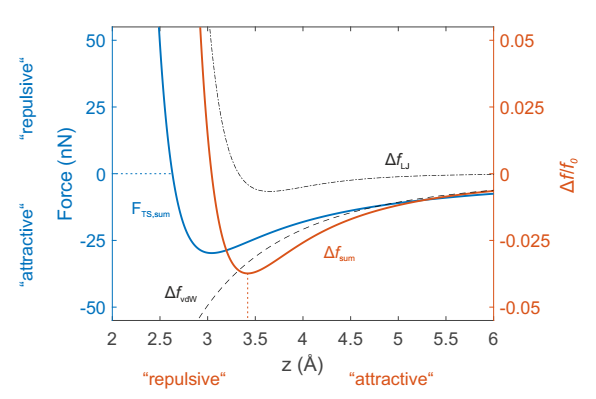
\includegraphics[width=0.7\textwidth]{./images/AFM-graph-martin}
		\label{fig:AFM-force}
\caption{Sketch of tip-sample interaction force (blue) together with relative frequency shift. Contributions of vdW and Lennard Jones like forces result in two separable frequency shifts $\Delta f_{LJ}$ and $\Delta f_{vdW}$ (black) that add up to a total of $\Delta f_{sum}$ (orange) from where the total force is derived. From \cite{schwarz_assembly_2018}}
\label{fig:AFM-sketch}%
\end{figure}

Amongst others, forces between AFM tip and sample are made up of attractive forces like van der Waals (vdW) forces and repulsive forces like mechanical contact force and Pauli repulsion.

vdW interaction is always attractive and described by
\begin{equation} \label{eq:vdW}
F_{vdW} = - \frac{A_H R}{6z^2}
\end{equation}
Here $A_H$ is the \textcolor{red}{\textbf{?}}, $R$ \textcolor{red}{\textbf{?}} and $z$ \textcolor{red}{\textbf{?}}. Although the strength quickly diminishes with distance $z$, vdW interaction is long range and thus always present in AFM measurements.

Mechanical contact force, Pauli repulsion and chemical bonding are given in the Lennard Jones (LJ) model.\cite{jones_determination_1924}
\begin{equation} \label{eq:LJ}
 F_{LJ} = - \frac{12 E_{min}}{z_0} \left ( \left (\frac{z_0}{z} \right ) ^{13} - \left ( \frac{z_0}{z} \right )^7 \right )
\end{equation}
$E_{min}$ is \textcolor{red}{\textbf{?}}.

The typical resulting force between tip and sample $F_{TS,sum}$ is artistically shown in \autoref{fig:AFM-sketch}. 
%On the top part a tuning fork with an atomic tip is shown on top of the sample surface. The interaction forces $F_{ts}$ act between tip and sample and are indicated by an arrow. In the lower part a representation of the resulting force in dependence of the tip-sample distance is shown. 
The sum of interaction $F_{TS,sum}$ between tip and sample is shown as blue  line. The attractive vdW force is plotted in dashed black curve. A typical frequency shift $\Delta f_{sum}$ is given as orange graph. The frequency shift $\Delta f$ is proportional to the force gradient acting on the tip.

$$\Delta f = - \frac{f_0}{2k_0}\frac{\delta F_{TS}}{\delta z}$$

One can distinguish different regimes as indicated by the labels. When tip and sample are in considerable distance to each other, the attractive vdW forces are the dominant part in the sum. While the tip approaches the sample, more and more interactions with the surface and adsorbate add to this force, increasing $F_{TS}$. When the separation reaches $z_0$, the distance becomes so small that repulsive forces overcome the attractive one at the boarder to the repulsive regime.

%AFM is used here in the non-contact mode (\textbf{nc-mode}): The tuning fork is driven at its resonance frequency with fixed amplitude and at a certain distance to the sample. Long-range forces like van-der-waals and others change the resonance frequency of the cantilever. This change is a indication of the acting force between cantilever and sample. 

AFM measures does not measure a mix of electronic and geometric information projected onto a 2D-map like in STM.

To increase the lateral resolution the tip can be functionalized with CO. This method is widely used \cite{albrecht_direct_2016, kawai_multiple_2018, kawai_atomically_2015, schulz_elemental_2018, gross_chemical_2009, pavlicek_generation_2017, schwarz_corrugation_2017} to investigate not only geometric features that are not directly accessible in STM, but also chemical differences on the sample.\cite{wang_exploration_2017}

\begin{figure}\centering
	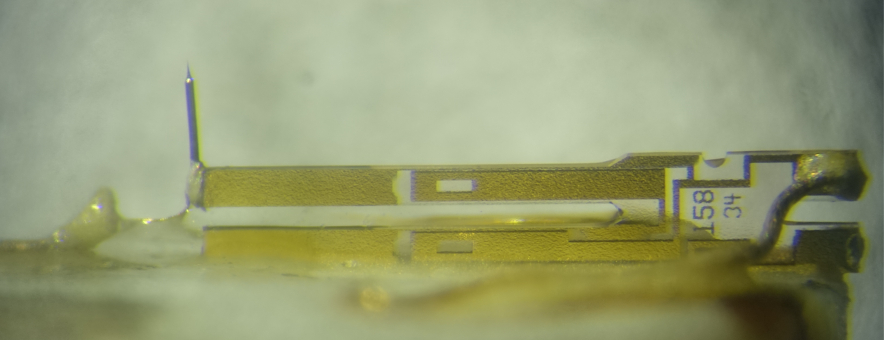
\includegraphics[width=0.7\textwidth]{./images/AFM-qplus-photograph}
	\caption{Photograph of the tuning fork and cantilever. The tip is glued to the tuning fork on the left side. From \cite{he_bottom-up_2017}}
	\label{fig:AFM-tuning-fork}
\end{figure}

\subsection{\textcolor{red}{\textbf{Experimental details}}}
The used LT-AFM features a tuning fork sensor, as shown in \autoref{fig:AFM-tuning-fork}. Here the tip is positioned below an oscillating fork.  A piezo element that continuously stimulates oscillations in a quartz crystal is used to drive the forced oscillation of the tuning fork ($f_0$, $k_0$). To its end the AFM/STM tip is attached and follows the oscillation with a fixed amplitude.

Measurements are done in the frequency modulated mode, meaning that the shift in resonance frequency, by an amount $\Delta f$  proportional to the force gradient, is recorded in constant height to show the proportional local force gradient. The image is created by raster scanning the surface like in LT-STM. The best images were recorded where repulsive contributions to $F_{TS,sum}$ arise. This is because repulsive forces are short range while attractive vdW interaction is long range and thus does not provide atomic contrast.

AFM experiments are done under ambient conditions (see copper foil characterization \autoref{fig:foil-afm-as-bought}) and in UHV at \SI{5}{\kelvin} at the LT-AFM (see functionalized coronene chapter \autoref{section:HBBNC}).

%\subsection{\textcolor{red}{\textbf{Methods}}}
%\textbf{$\Delta f $ images} 
%Contour lines in $\Delta f$ images represent lines with the same tip interaction strength.
%
%\textbf{$\frac{\Delta F}{\Delta z}$} spectroscopy is used to highlight changes in the local contact potential.
  \section{\textbf{C}hemical \textbf{V}apor \textbf{D}eposition}
	 %  this is a description of a cvd process usually used in this worl
There are two major ways to grow adlayers defined by their atomic constituents and certain stoichiometry in UHV, namely the chemical vapor deposition (CVD) or temperature programmed growth (TPG) of a precourser.

While the latter works by adsorption of the precourser onto the surface where it schould grow and activating the reaction via heating, the first uses a already hot surface to decompose the precourser on. 

\paragraph{CVD}\index{CVD}offers some advantages over TPG when it comes to homogenous growth of a monolayer. The precourses decomposes on contact with the hot substrate surface and its fragments for the adlayer. As time goes by, the adlayer grows in coverage and less free hot surface area is available for decomposing new ``building blocks'' for monolayer formation. If a monolayer is formed, no additional second layer is formed because of missing building blocks which only arise on contact with the uncovered substrate surface. Therefore this process is called self-limited.

While in CVD, the process of forming the adlayer (adsorption, decomposing, diffusion on surface upon coalescence with an already present nucleation seed, layer growth), TPG offers some other path of layer growth. Due to the fact that the surface is covered from the beginning with the desired number of molecules, the density of present building blocks at a certain time (and same dosage as with CVD) is higher. Therefore this growth experiences other results as CVD.

Hexagonal boron nitride grown on noble metals shows destinct differences between these two modes. CVD results in a more homogenous monolayer coverage than TPG and is therefore preferred.

The growth by itself is well investigated on transition metal surfaces \cite{gomez_diaz_hexagonal_2013,morscher_formation_2006}, on the copper and nickel surfaces \cite{preobrajenski_monolayer_2005,joshi_boron_2012}. Even more complicated samples can be created with this technique \cite{roth_chemical_2013} and the following gives a short introduction in the occuring processes.

\begin{wrapfigure}{l}{0.3\textwidth}
 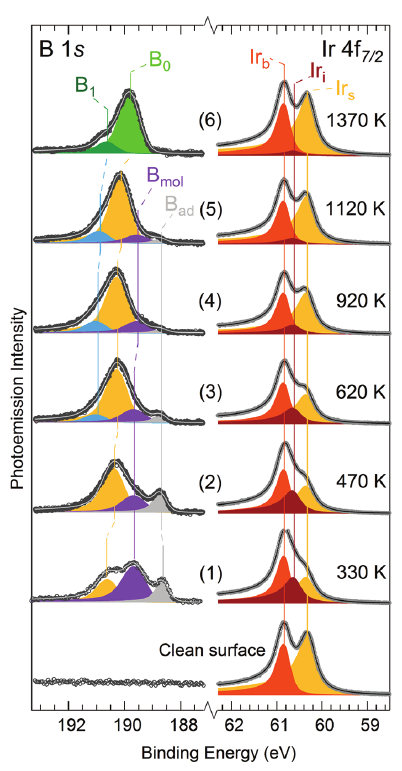
\includegraphics[width=0.9\linewidth]{./images/07571n_fig5.png}
 \caption{\cite{orlando_epitaxial_2012}}
\label{fig:borazine-TPG-on-Ir}
\end{wrapfigure}

Figure \ref{fig:borazine-TPG-on-Ir} shows a typical XPS spectrum of a TPG process with borazine adsorbed on a Iridium surface. At the graphics' bottom one can see the clean Ir surface with no borazine adsorbed (no sign of B1s). There are two contributions in the Ir-peak. While the low energy ($Ir_s$) peak stems from the surface atoms of the subtrate, $Ir_b$ denotes the contribution from the atoms in the bulk. Upon borazine adsorption $(1)$ a broad $B1s$ emerges accompanied with a new contribution in the $Ir$-peak which is a result of borazine-Ir interaction decreasing the intensity of $I_b$ and $I_s$ .

Upon annealing ($(2)$-$(6)$) this peak looses in intensity while the $I_b$ and $I_s$ recover to their initial position. Interesting changes happen to the $B1s$ peak. While at lower temperatures, several peak contributions can be distinguished, denoted as $B_{mol}$ for entire molecules and $B_{ad}$ for molecular fragments. With increasing temperature, $B_{mol}$ decreases for a increase in the $B_0$ peaks. At lower temperature (1), $B_{mol}$ decreases and $B_{ad}$ slightly increases. When exceeding 620K ($\approx \SI{350}{\celsius}$, (3)) a new peak emerges and develops into $B_1$ when increasing temperatures. When temperature is high enough the only peaks left are $B_0$ and $B_1$ - the two contributions of boron atoms stem from boron atoms interact with the Iridium substrate with different strength due to different registry to the substrate.

While usaually borazine is used as precourser different other options exist like B-Trichloroborazine (${ClBNH}_3$) \cite{auwarter_synthesis_2004-1}.
  \section{\textbf{S}canning \textbf{E}lectron \textbf{M}icroscopy}
	 Invented in the 1930's by Manfred von Ardenne\cite{ardenne_elektronen-rastermikroskop_1938}, Scanning electron microscopy (SEM)\index{SEM} is another versatile tool for the experimentalist. In contrast to (LT-)STM and AFM, SEM is capable of imaging huge areas of the sample within a very short time, which allows for a vast overview as well as good statistics. Magnifications reach up to 500k and above, illustrating even features in the order of \SI{1}{\nano \meter}.

As the name already discloses, SEM scans the surface with electrons. Their interaction with the material are diverse and some of them are explained in the following. While all effects are present in every measurement, not every microscope features detectors for all of these. While detectors for secondary electrons are standard equipment others may be not.

%\begin{itemize}
% \item \textbf{Secondary electrons (SE)} are produced in the bulk by the high energetic primary electon beam within close proximity to the surface. This is why SEMs offer a very good resolution of the surface itself.
%  \item \textbf{Backscattered electrons (BSE)} are elastically scattered primary electrons. The resolution of this mode is not as high for the secondary electrons. The intensity of the BSE depends strongly on the the atomic number Z of the specimen. It is useful for a complementary view, for example when chemical composition is of high interest.
%  Electron backscatter diffraction (EBSD) is used to achieve information on the crystallographic structure of a specimen.
% \item \textbf{Characteristic X-Rays} are used to identify the composition and measure the abundance of elements in the sample, too. See section \ref{sec:XPS} and figure \ref{fig:auger-core} therein for more details.
% \item \textbf{Cathodoluminescence (CL)} happens when electrons hit a material and exite photons. This effect is used in televesion screens where high energetic electrons are accelerated onto a screen containing phosphorus. There they distribute their energy with many others, some of those loose energy in form of photons which wavelenghts are within the visible spectrum. These light is called cathodoluminescence.
% \end{itemize}

The primary electrons are created with a filament. These often consist of tungsten (metal, high melting point, low work function). Alternatives are lanthanum hexaboride ($\textnormal{LB}_6$) - often used in LEED setups, too - or zirconium oxide.
Electrons are accelerated (typical energies are within \SIrange{1}{40}{\kilo \eV}) and focused on the specimen surface in a spot with few \si{nm} diameter with condenser lenses. Scanning the surface is achieved with coils that deflect the electron beam and therefore the actual scanning spot.

When the electrons hit the surface, they interact with the specimen in a small volume. The volume depends on the electron's energy, the atomic number Z of the specimen and the specimen's density. It is typically in the order of \SIrange{0.1}{5}{\micro \meter}.

Drawbacks:
\begin{itemize}
 \item[-] Sample has to be mounted $\rightarrow$ no in-situ measurement, surface alteration in between
 \item[-] Rather ``dirty'' vacuum $\rightarrow$ surface alteration while measuring
 \item[-] Measurement destroys sample $\rightarrow$ adsorbate build-up due to chemical reaction below e-beam
\end{itemize}


  \section{\textbf{S}canning \textbf{T}unneling \textbf{M}icroscopy}
     The tunneling effect occurs when a particle faces a potential barrier. In the classical picture the particle is prohibited to move across the potential barrier if the particle's energy is lower than the barrier height. In quantum mechanics however, the particle is described as wave. When this now faces the potential barrier, a fraction of the wave package is transmitted through the barrier - an effect called tunneling.

\subsection{An historic overview}
The tunneling effect was first observed by Hund in 1926 in molecules, where he explained the sharing of an electron between atoms, each separated by a potential well.\cite{Mehra_tunneling_1982} A principle fundamental for an understanding of covalent chemical bonds. 

The first quantitative expression of the tunneling current between two vacuum separated metals was introduced by Bardeen in 1961.\cite{Bardeen_tunneling_1961} 

This lead to an early experiment build by Russell Young, John Ward and Fredric Scire in 1972.\cite{Young_topographiner_1972} Here tunneling with metal tip was shown already. The concept was further improved by Binning \& Rohrer in 1981 when they were the first to report experimental evidence for the tunneling through an vacuum gap.\cite{binning_tunneling_1982} They showcased the excelled resolution capabilities by resolving the ($7 \times 7$) reconstruction of the Si(111) surface \cite{binnig_1983} and received the noble prize in 1986 for "their design of the scanning tunneling microscope" (STM).\cite{_noble_price_1986} 

In the following the tunneling process through a vacuum gap between metallic tip and sample will be summarized, addressed theoretically and used to describe the basic concept of STM.

\subsection{Basic principles}
\index{STM!One dimensional tunneling}

\begin{figure}[]\centering
	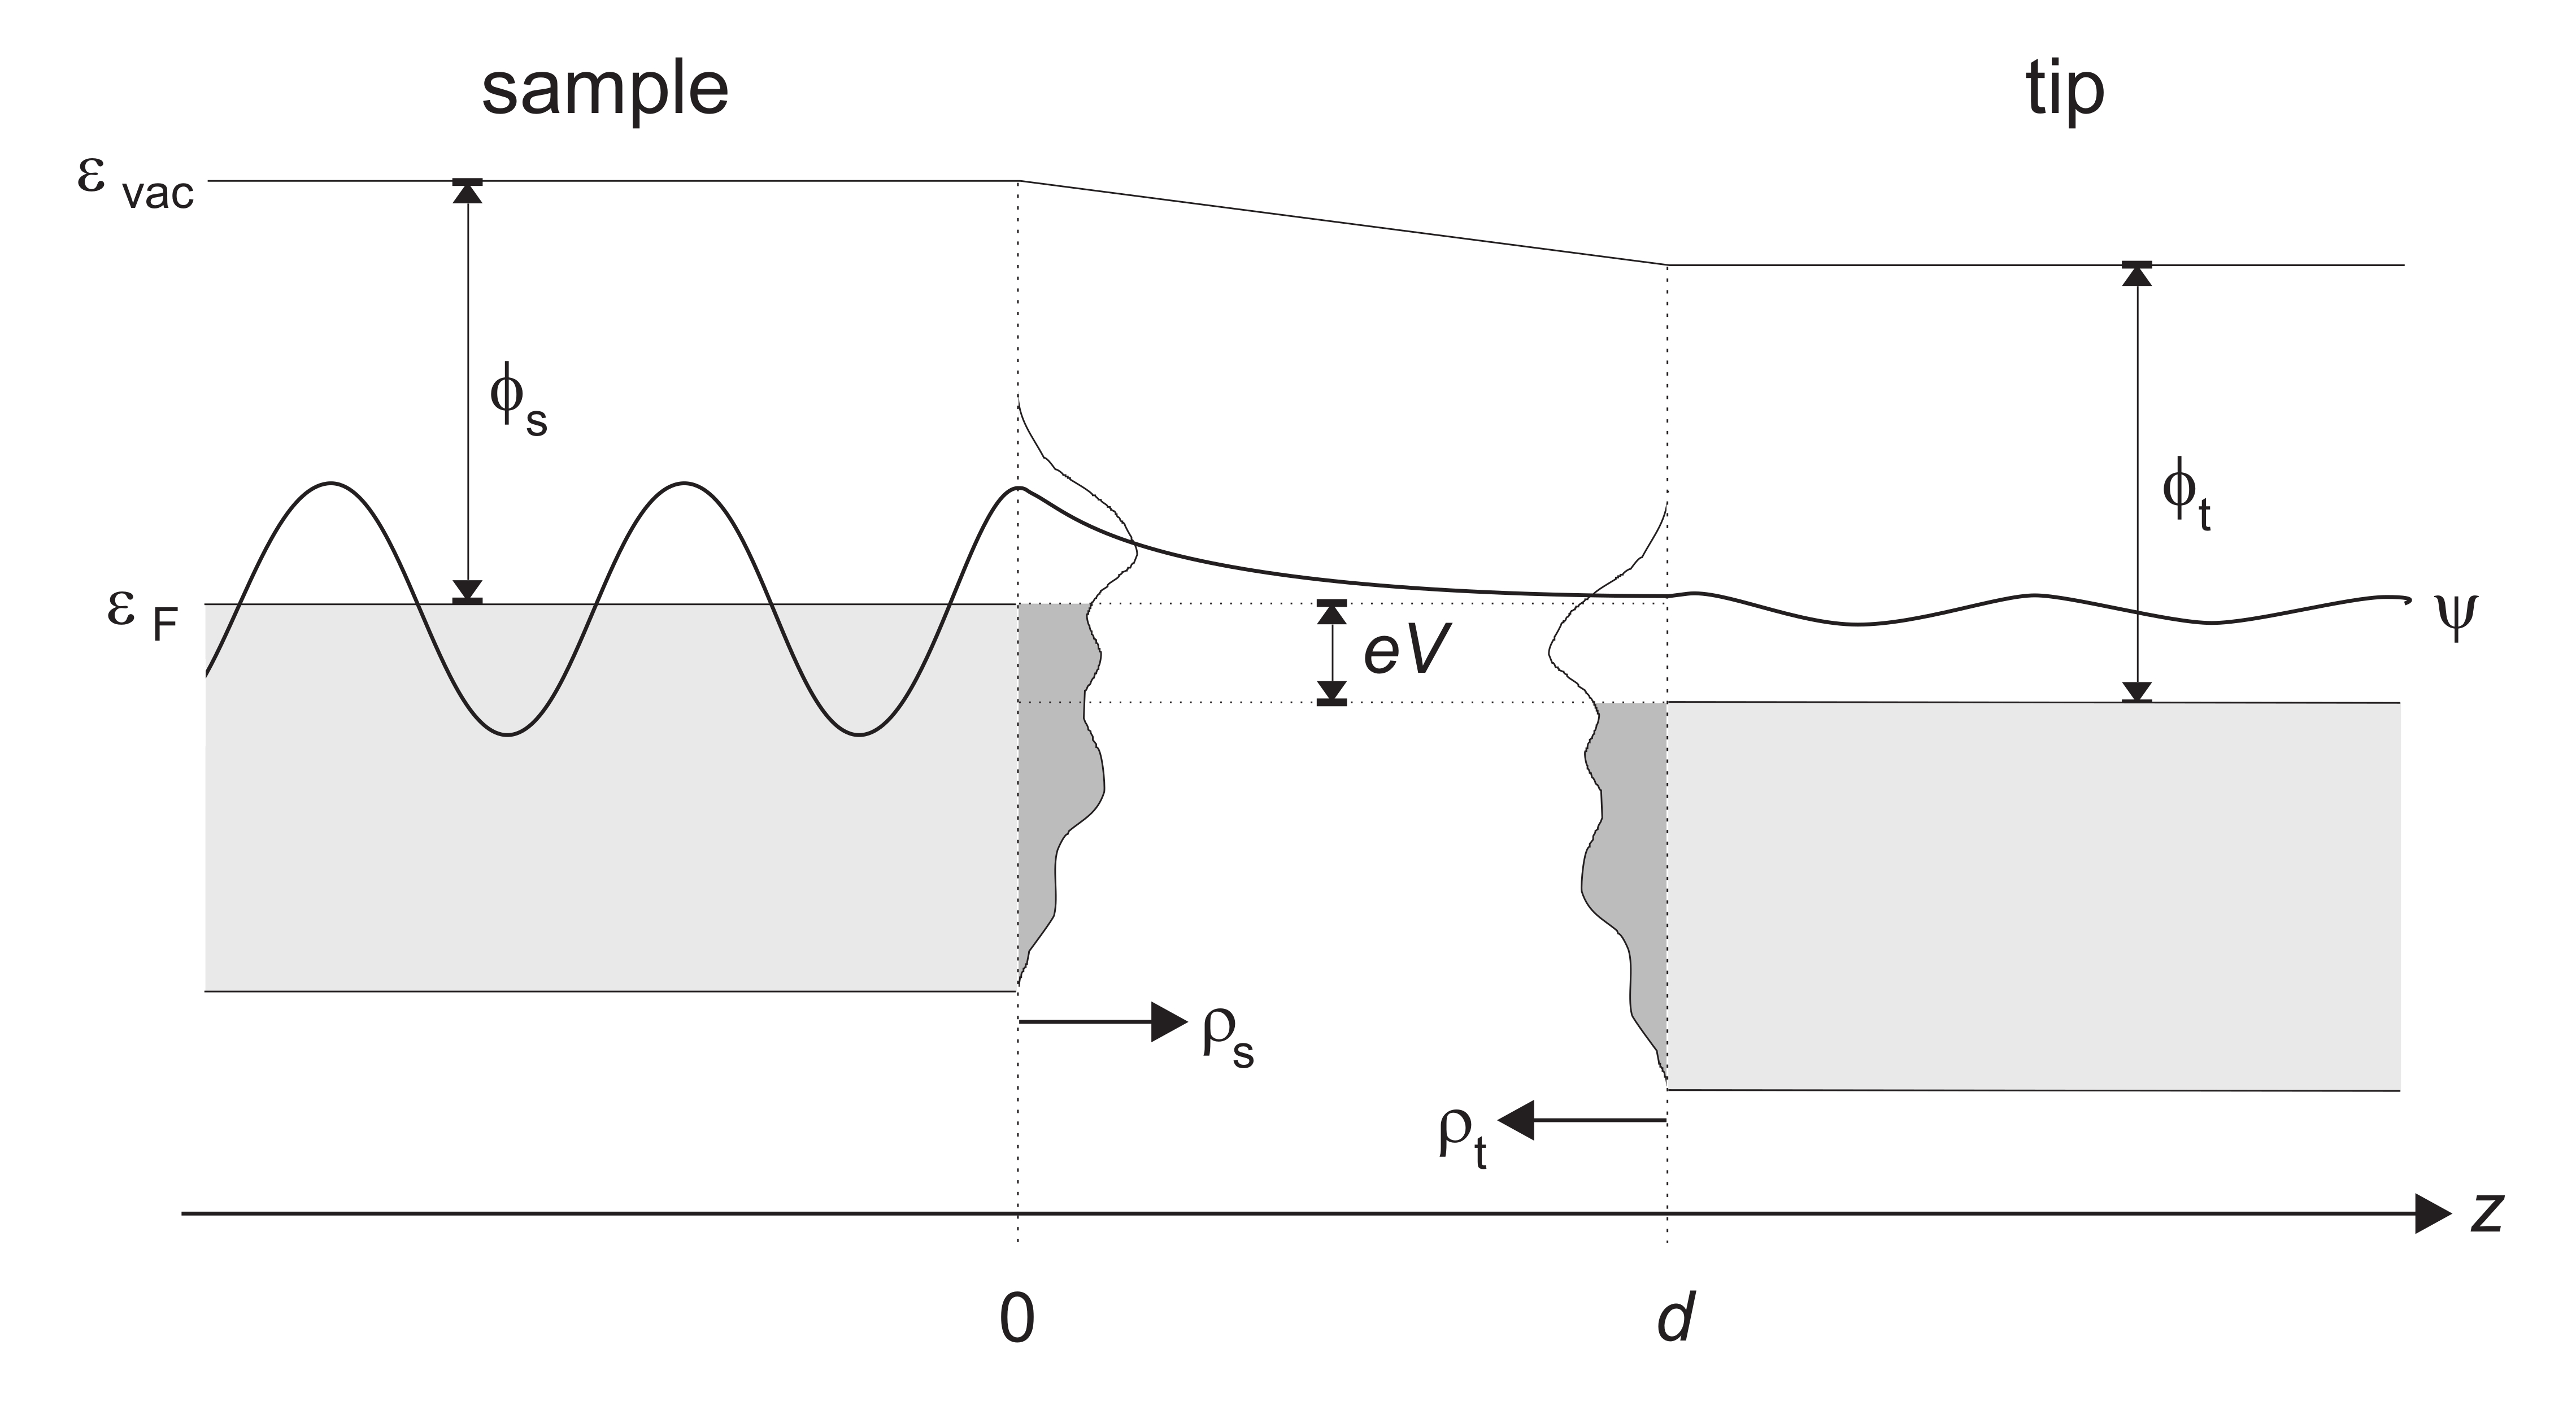
\includegraphics[width=0.7\textwidth]{./images/tunnel-barrier}
	\caption{Energy diagram to visualize the tunneling process between sample (left) and tip (right) separated by a distance d. Work functions of sample and tip ($\Phi_s$ and $\Phi_t$) separate the filled states (shaded regions) and the vacuum level ($\epsilon_{vac}$). Since sample ($\rho_s$) and tip DOS ($\rho_t$) may not be uniform, a fictional DOS is sketched in darker colors between both. The samples energy is lifted by $eV$ after a bias is applied and results in a net electron current from the sample into the tip. One tunneling process is indicated by a wave function $\Psi$ in the sample. After overcoming the vacuum barrier its amplitude decreased and the corresponding electron occupies a free state (white) in the tip material.  Adopted from \cite{diss-schunack}}
	\label{fig:STM-barrier}
\end{figure}

Consider a system where two metals (sample and tip) are separated by a vacuum gap. 

The amount of energy needed to remove an electron from the metals highest occupied energy level ($E_F$, Fermi energy) is called work function $\Phi$. It depends on the electrostatic potential $\phi_E$ that has to be overcome by an electron charge $e$ at the surface.
$$ \Phi = -e \phi_E - E_F $$

\autoref{fig:STM-barrier} shows an energy diagram for tip and sample. The work function $\Phi_s$ (sample) and $\Phi_t$ (tip) separates the vacuum level $\epsilon_{vac}$ and Fermi energy $E_F$.

If sample and tip are in thermodynamic equilibrium, their Fermi energies are equal.
When both are brought in close contact, electrons from the sample tunnel into unoccupied states of the tip and vice versa in the same number. Hereby electrons close to $E_F$ have the largest decay length and attenuate less strong in vacuum and contribute strongest to the tunneling current. This current can be modeled and calculated in simple systems. 

%\paragraph{STM}
In the model of Tersoff-Hamann\index{STM!Tersoff-Hamann}\footnote{Please's note that there are more models and corrections to them. An evolution from Bardeen's approach to the one done by Tersoff-Hamann can be found here \cite{lounis_theory_2014, wortmann_interpretation_2000} including Chen's expansion.} the tip is atomically sharp and its electrons waveform is s-like. Further assuming low temperature and a constant band structure for the tip with apex radius R, it is possible to calculate the tunneling current $I$. 

$$I \propto U \cdot \rho_t(E_F) \cdot \rho_s(E_F) \cdot \kappa^{-4}R^2e^{2\kappa R} $$

With this theory constant current STM images image the surface density of states for  a given voltage $U$. The exponential decay ($\propto e^{-\kappa d}$) of an electron wave function into vacuum is characterized by $\kappa=\frac{\sqrt{2m\Phi}}{\hbar}$. It limits the current, which is proportional to the squared amplitude of it. 

$$I\propto e^{-2\kappa d}$$

Like in one dimension the current depends on the barrier height $\Phi$ through $\kappa$. Increasing the distance exponentially decreases the tunneling current.\footnote{http://pmrb.free.fr/work/diplom/html/mainse2.html} This exponential relation is the reason for the excellent topography resolution capabilities of STM.

While its a good first approximation of the system, in many cases more than just the electrons near Fermi contribute. Also a uniform $\rho_t(E)$ may not be accurate in all cases.

Using \index{STM!WKB} Wentzel-Kramers-Brillouin (WKB) theory\cite{wentzel_verallgemeinerung_1926, kramers_wellenmechanik_1926, brillouin_mecanique_1926} the tunneling current is given by
\begin{equation}
I=\int_0^{eV}\rho_s(r,E)\rho_t(r,eV+E)T(E,eV,r)dE
\label{WKB}
\end{equation}
where $\rho_s(\rho_t)$ is the density of states of the sample (tip) and T is the tunneling transmission probability
\begin{equation}
T(E,eV)=exp\left(-\frac{\textcolor{red}{\textbf{2}}Z\sqrt{2m}}{\hbar}\sqrt{\frac{\Phi_s+\Phi_t}{2}+\frac{eV}{2}-E}\right)
\label{Transmission-function} 
\end{equation}
describing the probability of an tunneling event between tip and sample.

The samples potential can be changed by applying a voltage $V=U_b$ (bias) to it. This lifts its Fermi energy with respect to the tips and leads to a net electron current from the sample into the tip. Reversing the voltage results in electrons tunneling from the tip into the sample. If $eV<0$ the tunneling current is largest for $E=0$ (electrons on the Fermi-level of the sample), if $eV>0$ the tunneling current is largest for $E=eV$ (electrons of Fermi level in tip).

Due to the fact that the tunneling current is proportional the density of states in the tip and the molecule one can deduce the band structure within a range of several volts in the vicinity of the Fermi energy. Investigation of this behavior led to the establishment of a new measurement technique, called scanning tunneling spectroscopy (STS).

\subsection{\textbf{S}canning \textbf{T}unneling \textbf{S}pectroscopy}
\label{section:STS}
Changes of the tunneling current with the bias voltage were observed by Tromp et al. in 1986 \cite{tromp_atomic_1986}. They discovered a change in contrast when scanning a SI(111) surface with either positive or negative bias. The change in contrast is most apparent in semiconductors and semi metals\cite{bonnell_scanning_1993}, but adsorbates and charged areas of the sample change the DOS locally and therefore the contrast in STM. While simple results may be already obtained by comparing two images recorded at different biases, more detailed information can be achieved.

\index{STS!Bias below work function}
If tunneling conditions are such that $eV\leq\Phi$, observed features in $dI/dV$ are associated with the surface DOS. Critical points in the surface projected DOS give rise to features in dI/dV. Interpretation of these features with the WKB theory (i.e. differentiating equation \eqref{WKB}) gives
$$dI/dV=\rho_s(r,eV)\rho_t(r,0)T(\textcolor{red}{\textbf{eV}},eV,r)+\int_0^{eV}\rho_s(eV)\rho_t(r,E-eV)\frac{dT(E,eV,r)}{dV}dE$$
The first term contains the DOS of the sample and tip and the transmission function. While it is usually unknown, a closer look to \eqref{Transmission-function} indicates a smooth, monotonically increasing function in V. This mannered dependence on V gives a smooth background described by the second term $\int_0^{eV}\rho_s(eV)\rho_t(r,E-eV)\frac{dT(E,eV,r)}{dV}dE$.
The first term $\rho_s(r,eV)\rho_t(r,0)T(\textcolor{red}{\textbf{eV}},eV,r)$ describes the dependence on the DOS in the sample for energies $eV$ - our desired spectrum. As for STM topography images, bias voltage can be chosen to either probe occupied ($U_b < \SI{0}{\volt}$) or unoccupied states ($U_b > \SI{0}{\volt}$).  At low temperatures the vanishing lateral movement of adsorbates makes them also accessible to tunneling spectroscopy with sub molecular lateral resolution. It is possible to deduce the electronic configuration with atomic spatial resolution.

\subsection{Machine description and experimental details}
The success of STM and STS is promoted by good mechanical engineering. Since distances down to the atomic length scales are investigated, the experiment needs a careful set up. This is true especially for damping of external vibration that would otherwise conflict with the measurement. Sufficiently low partial pressures are needed to achieve little contaminant adsorption and the long investigation times associated with it.

Since all used UHV chambers have many common parts, a typical setup is described with the low temperature (LT) STM setup. Here the most experiments were carried out.

The central part of the LT-STM setup is the commercial \textbf{Beetle-type STM scanner} \cite{zoephel_aufbau_2000} as shown in \autoref{fig:stm-heliocoidal-ramp}. Here a helicoidal ramp carries the central scan piezo with attached STM tip. Three outer piezo tubes are used in slip-stick motion to circularly move on the ramp. Because the ramp is cut with an inclination of \SI{2}{\degree} the circular motion of the piezos results in the STM tip moving up and down. This is used to control the height above the sample during tip approach and macroscopic lateral movement.

A separate piezo is used to control the lateral position of the tip during scanning. With it the image width, scan speed and tip-sample distance can be controlled on a continuous, sub-atomic length scale (\autoref{fig:STM-tip}).

Not only the macroscopic movement of the STM stage is controlled with a set of piezos, but the position of the tip (x, y, z) during scanning, too (see \autoref{fig:STM-tip}). In this work a segmented tubular piezo is used to control the tips position. The piezos elongation can be controlled with the voltage applied to them, which is used to choose not only the tip-sample distance. Lateral movement is done by addressing its four segments. Each is used to control movement along $\pm \textnormal{x}$ and $\pm \textnormal{y}$ direction and controlled by the feedback loop. For recording an image the area is raster scanned in consecutive lines, applying a sawtooth voltage to the fast scan direction. The next lines are chosen by stepwise increasing the voltage along the slow scan direction. Other parameters like image size and scan speed are controlled wit the piezos as well.

The measured current is translated into a voltage (I/U converter) and processed in a 20 Bit digital $\rightarrow$ analog (D/A) converter. The current intensity is feed into the Digital signal processor (\textbf{DSP}) board. Here the STM Software's current set point is compared with the measured value. The tips position is controlled with a feedback loop. If the tips position needs to be corrected, a voltage is passed through a HV amplifier and is applied to the corresponding piezo element. 
%The DSP is used to attenuate high frequency components. \textcolor{red}{\textbf{ More detail?}}

Differentiation of the current signal is done with an \textbf{Lock-In Amplifier}. Here the spectrum is not recorded directly by sweeping the bias and numerically differentiating the measured current. A sinusoidal modulation on top of the bias voltage with a frequency higher than the low pass frequency of the DSP is used. The modulated bias leads to a tunneling current modulation with the same frequency. The differentiation is performed by reading the AC current signal with the same frequency as the modulation which directly gives the dI/dV signal and therefore the DOS of the sample at $U_b$. 

Because the Lock-In Amplifier then only takes signals with the same frequency than the excitation frequency into account, the results are much less suspect to noise. Compared to numerical differentiation, a Lock-In needs less computing effort, too. It is important to note that the DSP does not recognize the bias/current modulation as topographic feature and regulates as without modulation. If the modulation frequency is too low, the feedback tries to compensate the modulation by changing the distance to the sample. If the modulation frequency is too high, the capacitance between tip and sample leads to an $90\deg$ phase shifted current which increases with modulation frequency. One usually chooses the modulation frequency slightly above the cutoff frequency for the feedback loop.

\begin{wrapfigure}{O}{5cm} \centering
	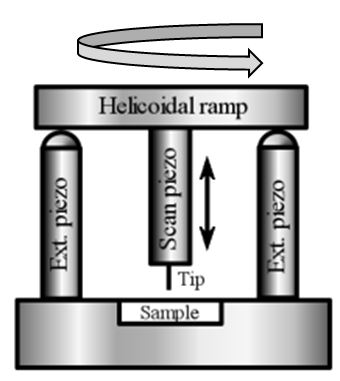
\includegraphics[width=4cm]{./images/STM-sketch-2}
	\caption{STM sample stage to control the tip position. The coarse movement is controlled by exterior piezos. Each moves on a heliocoidal ramp with slip-stick motion. The precise positioning during scan is done with a central piezo to which the tip is attached. Modified from \cite{heliocoidal_ramp_2018}.}
	\label{fig:stm-heliocoidal-ramp}
\end{wrapfigure}

To maintain UHV conditions, a set of pumps is used. For the preparation chamber, where high partial pressures occur during sample cleaning and preparation, a combination of roughening and turbo molecular pumps is used. First a roughening pump lowers the atmospheric pressure to \SI{1}{\milli \bar}. With this pressure on the outlet side a turbo molecular pump is used to decrease the pressure even further to the  \SI{1e-8}{\milli \bar} range. The remaining pressure is caused by adsorbate covered chamber walls where continuous ad-/desorption takes places and maintains a pressure equilibrium. After heating the entire chamber to temperatures above \SI{120}{\celsius} while constantly pumping, most of the water is desorped from the walls and pumped. After cooling down to room temperatures, the pressure settles in the \SI{5e-10}{\milli \bar} regime.

As the pumping efficiency of turbo molecular pumps decreases for low pressures, each chamber is equipped with an ion getter pump. Here a high voltage \SIrange{1}{7}{\kilo \volt} is applied between two getter materials. Residual gas particles ionize in the strong electric field and are accelerated towards the plates. Here they impinge with high velocity and are buried deep in the plate material that they can't leave. The reduced number of residual gas particles results in a lower pressure.

To further reduce the number of potential contaminations, parts of the chamber can be cooled down with liquid nitrogen. Because of the great temperature gradient, gaseous residuals condense on the much colder surface of the cooling trap and remain adsorbed while the temperature is kept low. Without refilling with liquid nitrogen the temperature slowly increases over time, so that the cooling trap looses pumping efficiency over time (usually after \SIrange{1}{2}{\hour}) and starts to release trapped contaminants again.

A titanium sublimation pump is installed to evaporate titanium on demand. This covers the chamber walls and, due to its reactivity, binds residual gas. After some time the reactivity diminishes and a new layer has to be evaporated. With routine operation intervals the base pressure of the UHV system can be improved permanently.

While LT-STMs may be operated with solely helium, it is more resource saving to only cool the direct proximity of the sample and the STM with He and to suppress the heat flow out of the He cryostat with a second surrounding nitrogen cryostat (boiling point: \SI{77}{\K}, compare figure \ref{fig:STM-cryo}). This diminishes consumption of globally limited He. To maintain a temperature of \SIrange{5}{7}{\K}, one to two liters of liquid helium are evaporated a day, plus an additional amount of three to four liters liquid nitrogen. Evaporated helium is reclaimed in a closed circuit with a system of purifying and storage/cooling steps so that only a small amount of helium escapes the circuit and is lost.

Sample temperatures down to \SIrange{5}{7}{\K} allow for observations not possible at elevated temperature. Cooling not only reduces thermal drift in the piezo elements that are used to control the tip's position on the sample. Thermal energy at low temperature is not high enough for atoms or molecules to move on most substrates. Species mobile at room temperature (and therefor not representable at room temperature in the sub-ML regime) become immobile and accessible for ST microscopy and spectroscopy. ST spectra resolution is better at low temperatures.

\begin{figure}[ht]\centering
	\subfigure[LT-STM setup. Different functional groups are highlighted by colors. A low base pressure in achieved with a combined pumping system comprised of ion pumps and turbo molecular pumps (cyan). The liquid helium/nitrogen bath cryostat (red) is used to maintain low temperatures. Sample holders are operated with a rote able, variable temperature manipulator (green). Sample preparation is done in the preparation chamber (blue). After transfer to the LT-STM chamber (yellow) a gate valve is used to seal the LT-STM from remaining residual gas that may be present in the preparation chamber. Vibration isolation of the frame is achieved with legs floating on pressurized cylinders (orange).]{
		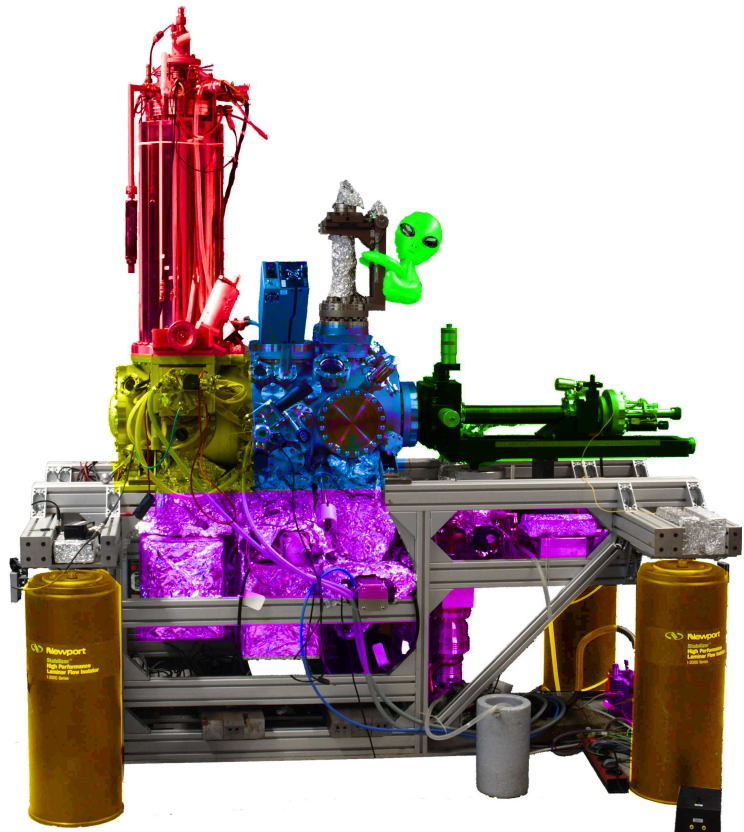
\includegraphics[width=0.45\textwidth]{./images/chamber-sketch.jpg}
		\label{fig:chamber-sketch}
	} \quad
	\subfigure[Scheme of a liquid bath cryostat. While in the inner stage a temperature of \SIrange{5}{7}{\K} is achieved with a liquid helium reservoir, an outer liquid nitrogen cryostat is used to isolate the inner cryostat from the surrounding room temperature and to reduce the amount of liquid helium used to maintain cryogenic temperatures.]{
		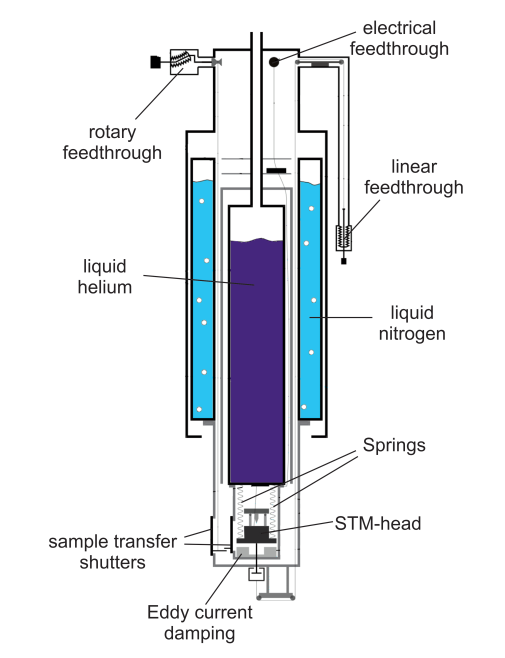
\includegraphics[width=0.45\textwidth]{./images/sketch-cryo.jpg}
		\label{fig:STM-cryo}
	}
	\caption{Typical setup for low temperature measurements. A vibration isolated UHV chamber is used to prepare samples and investigate them in a separable chamber with either STM or AFM. A liquid bath cryostat is used to maintain low temperatures. Images adopted from \cite{diss-knud}}
	\label{fig:STM}
\end{figure}

\begin{figure}\centering
	
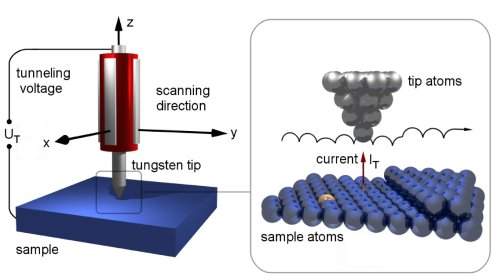
\includegraphics[width=0.6\textwidth]{./images/stm-rutgers-modified.jpg}
	\caption{Operating principles of an STM. A macroscopic sketch  shows the central piezo that controls the tip position on the sample. The piezo is divided in four parts to control movement in the x-y plane and tip-sample distance. A microscopic sketch shows the tips movement in constant current mode while moving across a atomic step edge. Here the tip is retracted to maintain a constant current, which in turn leads to a larger apparent height in STM. Note the single incorporated alien atom. Although its height is the same as its neighbors, STM records the change in DOS. Less electrons tunnel and the apparent height on the terrace is reduced above the alien atom. Adopted from \cite{STM-rutgers}}
\label{fig:STM-tip}
\end{figure}

Two damping stages are used, one for the chamber and a sequential one for the STM.

First the whole UHV system is placed on air pressurized cylinders. These can be lifted on demand, so that the chamber floats on four dampers and external vibrations/shocks are damped. 

A second stage decouples the sensitive STM scanner from the rest of the setup. First the complete STM stage hangs on springs to further limit the direct influence of vibrations. Second the remaining oscillation amplitude is damped by a eddy current damping. It is made of three magnets in close proximity to the surrounding conductor so that eddy currents are induced for each movement. The eddy current is typically larger at cryogenic temperatures, that results in a damping that works best at low temperatures. The kinetic energy of the oscillating system is transferred by the eddy currents into heat within the surrounding support. The heat is then mitigated by the external cooling of the cryostat.

\paragraph{Experimental details}

\textbf{Topography images} are created by raster scanning the surface pixel by pixel. 
We use the constant current (cc-STM) operating mode where the tips height is controlled to achieve a constant tunneling current as shown in \autoref{fig:STM-tip}. The regulating voltage on the height control piezo is recorded and plotted in an color-scale for each pixel. The brighter the color, the more the piezo had to retract the tip to maintain a constant tunneling current. Regions with the same DOS thus appear in the same contrast.

%	A modified tip allows for real space imaging of molecular orbitals.

\textbf{dI/dV} is performed in two ways - on single points (spectrum) and on areas (map). 

\textbf{Single point spectra} are used to measure electronic properties like molecular orbital energies and electronic band gaps.
Spectroscopic information can be obtained by either changing the bias voltage and tip height (I(V,z)-spectroscopy) or the tip-sample distance (V(z)-spectroscopy) (I=const).   

\textbf{Spectral maps} at a fixed bias show real space distribution of electronic states at the DOS that corresponds to the chosen bias. The signal intensity represents the differential conductance $\propto$ DOS. Differentiation is done with a Lock-In (see paragraph above). For dI/dV maps the feedback loop that controls the tip vertical position is not in use, so that the tip maintains an even height.

\textbf{Lateral manipulation} of atoms and molecules is possible with the STM tip. With a matching current/voltage setpoint, the tips vertical position can be chosen such that the tip interacts with the adsorbate. Lateral displacement of single molecules within molecular assemblies is only possible if molecule-molecule interactions are weak, e.g. no covalent bonds are formed between molecules. 

\subsection{Limitations}\index{STM:resolution}

The accuracy of a STM is very high with spatial resolution down to the atomic scale.

\textbf{Lateral resolution} with the STM depends on the tip shape and termination. A tip with single atom termination records sharp topography images. When there is more than one atom in the tip apex participating in the tunneling process lateral resolution decreases and each creates its own image with partial overlap.

\textbf{Spectral resolution} is influenced most by the tip DOS. Before each measurement a reference spectrum is recorded on the metal surface to ensure the the DOS fo the tip in metallic and does not show unexpected additional states that are typically induced by a modified tip.

Due to the fact that the tips motion is controlled with different piezos, one has to take different elongations in different directions into account. For example, if the STM scans the fast scanning direction just a bit further than the slow scan direction, the resulting image (although pixel wise square) is no longer physically square anymore. 
%Imagine a square (1:1 side ratio, diagonal angle 45\textdegree) where one side is elongated by 5\%. The resulting square (1:1.05 side ratio, diagonal angle 43.6\textdegree) looks square because it has the equal number of pixels in both directions, but it is physically rectangular. The expression used to calculate the uncertainty with known calibration parameters is
%$$\Delta \Theta = 45 - \frac{180}{\pi}\cdot\arctan(\frac{1}{1+x})$$ where x is the percentage of one side being longer. This results in an uncertainty of 0.3\textdegree(1\%), 1.4\textdegree(5\%, see example above), 2.7\textdegree(10\%). 
For moderate shear below \SI{5}{\percent} however, conformity is almost conserved and the angular uncertainty below \SI{1.5}{\degree}.

Because STM is sensible to electronic changes, it may change the footprint of an adsorbed compound \cite{sautet_interpretation_1992}. When laterally approaching an adsorbate this results in an additional tunneling current, because now electrons do not only tunnel directly into the substrate but through the adsorbate as well. Interferences between both tunneling processes depend on the adsorbate's orbital-symmetry and tip-shape. Local density of states calculations \cite{tersoff_theory_1985, lang_theory_1986, eigler_imaging_1991} are not adapted to grasp this effect since the tip is considered far away from the surface. Moreover, the tip radius or the tip-substrate distance is often optimized to fit the lateral size of the adsorbate print with the experimental image \cite{tersoff_theory_1985, eigler_imaging_1991}. 

The tip termination was changed in different ways. 
1. \textbf{Tip forming:} 
		A voltage pulse ($U_b \leq \SI{10}{\volt}$) is given for a short time ($t \leq \SI{1}{\second}$) when the tip is in tunneling contact. The intense current pulse reorders the tip termination.
2. \textbf{Vertical over-approach:}
		The tip is pushed into the sample surface in order to remove tip adsobates.
3. \textbf{Field emission:}
		An external power supply is used to apply a voltage ($U_b$=
		\SIrange{100}{500}{\volt}) between tip and sample. A serial resistor limits the current through the connected internal wires. Tip and sample are brought in close proximity to enable the tunneling process. Because of high electrical field strengths at the tip apex strong forces occur. Depending on the polarity the tip can either aggregate sample surface atoms or expel tip atoms. Careful distance increase then builds up a new tip apex.
The above mentioned ways are done with the tip remaining inside the STM.
4. \textbf{Tip sputtering:}
		To reorder the tip structure and to remove adsorbates accelerated Ar$^+$ ions are used. Because of higher partial pressures needed for sputtering the sample is transferred from the LT-SMT into the preparation chamber.

Mechanical and thermal vibrations limit the resolution of STM and STS, too. Therefor the damping stages that decouple the STM from the surrounding are important but may not always filter all mechanical vibrations. 

Signal wires are well shielded against electromagnetic radiation. Since the signal is transmitted with cables an external radio signal may otherwise couple into the wire and tamper with the signal.

Although STM works at room temperature, additional cooling may be applied to reduce the thermal vibrations.

STM is not capable to discern different elements. As complimentary method, X-Ray photoelectron spectroscopy is used for chemical identification of adsorbates.
     \subsection{\textbf{S}canning \textbf{T}unneling \textbf{S}pectroscopy}
 	 	\label{section:STS}
First changes of the tunneling current with the bias voltage were observed by Tromp et al. in 1986 \cite{tromp_atomic_1986}. They discovered a change in contrast when scanning a SI(111) surface with either positive or negative bias. The change in contrast is most apparent in semiconductors and semi metals\cite{bonnell_scanning_1993}, but adsorbates and charged areas of the sample change the DOS locally and therefore the contrast in STM. While simple results may be already obtained when comparing two images recorded at different voltages, more detailed information can be achieved. At low temperatures the vanishing lateral movement of molecules makes them also accessible to tunneling spectroscopy. It is possible to deduce the electronic configuration on with atomic spatial resolution.

Spectroscopic information (information on the DOS) can be obtained by either changing the bias voltage (I(V,z)-spectroscopy) or the tip-sample distance (V(z)-spectroscopy).  

Therefore the bias is modulated with a sinus like waveform. \index{STS!modulation}The frequency of the low amplitude modulation of the DC bias is much larger than the feedback loop frequency (\SIrange{1}{2}{\kilo \hertz}). The AC part of the tunneling signal is than recorded with a lock in amplifier. The in-phase component is directly the $dI/dV|_{V=V_{bias}}$, recorded simultaneously with the topography.\footnote{If the modulation frequency is too low, the feedback tries to compensate the modulation by changing the distance to the sample.	If the modulation frequency is too high, the capacitance between tip and sample leads to an $90\deg$ phase shifted current which increases with modulation frequency. One usually chooses the modulation frequency slightly above the cutoff frequency for the feedback loop.}

\index{STS!Bias below work function}
First let us consider small biases.
If tunneling conditions are such that $eV\leq\Phi$, observed features in $dI/dV$ are associated with the surface DOS. Critical points in the surface projected DOS give rise to features in $dI/dV$. Interpretation of these features with the WKB theory (i.e. differentiating equation \eqref{WKB}) gives
$$dI/dV=\rho_s(r,eV)\rho_t(r,0)T(\textcolor{red}{\textbf{eV}},eV,r)+\int_0^{eV}\rho_s(eV)\rho_t(r,E-eV)\frac{dT(E,eV,r)}{dV}dE$$
The first term contains the DOS of the sample and tip and the transmission function. While it is usually unknown, a closer look to \eqref{Transmission-function} indicates a smooth, monotonically increasing function in V. This mannered dependence on V gives a smooth background described by the second term $\int_0^{eV}\rho_s(eV)\rho_t(r,E-eV)\frac{dT(E,eV,r)}{dV}dE$.
Because T is smooth and monotonic the first term $\rho_s(r,eV)\rho_t(r,0)T(eV,eV,r)$ introduces the dependence on the DOS in the sample for energies $eV$ - our desired spectrum.

If $dI/dV$ is recorded simultaneously with the topography, another contribution arises. One usually observes an decrease in atomic corrugation when the distance between tip and sample is increased. The surface looks flat. To have the same tunneling current on atom positions and in between, the decay length in the valleys $\kappa_v$ must be larger than on the atom positions $\kappa_a$. The Z-depended corrugation given by Tersoff-Hamann is $$\Delta(Z)\approx \frac{2}{\kappa}e^{-\frac{\pi^2Z}{a2\kappa}}$$ where a is the lattice constant and $\kappa$ the inverse decay length. To make both a flat looking surface one gets the expression
$$\kappa_v=\kappa_a-\frac{2\pi^2}{\kappa a^2}e^{-\frac{\pi^2\bar Z}{a2\kappa}}$$ 
As the transmission factor changes with the decay length, the tunneling current and with it the $dI/dV$ changes. This is the origin of topographic features in $dI/dV$ maps when recorded at constant current.

The origin of the strongly voltage depended background can be found in WKB theory as well.
When writing the tunneling current as 
$$ I=\int_0^{eV}\rho_s(r,E)\rho_t(r,eV+E)exp\left(-\frac{\textcolor{red}{\textbf{2}}Z\sqrt{2m}}{\hbar}\sqrt{\frac{\Phi_s+\Phi_t}{2}+\frac{eV}{2}-E}\right)dE $$
the tunneling current reduces to 
\begin{equation}
\bar I=\rho_s\rho_t \bar V exp\left(-\frac{\textcolor{red}{\textbf{2}}\sqrt{2m}}{\hbar}\sqrt{\Phi}Z\right)
\label{tc}
\end{equation}
Assuming that DOS of tip and sample $\rho_t/\rho_s$ are constant, as well as discarding the change of the tunneling barrier with the bias voltage(an assumption only valid for very small voltages with $eV<<\Phi$) the derivative of \eqref{tc} is given by
$$\frac{dI}{dV}=e\rho_s\rho_texp\left(-\frac{\textcolor{red}{\textbf{2}}\sqrt{2m}}{\hbar}\sqrt{\Phi-\frac{eV}{2}}\right)Z$$
Substituting Z with the one obtained by \eqref{tc} leads to $dI/dV= \bar I / \bar V$ - which diverges as  $1/V$ when going to very low bias voltages and gives another contribution to the background. This makes it hard to observe features in close proximity to the fermi level ($V_{bias}=\SI{0}{\volt}$). This background can be reduced when operating at constant tunneling resistance and not at constant current. When doing this, features usually obscured by the $1/V$ diverging background can be observed.\footnote{A comprehensive overview on measurement technique and analysis can be found in \cite{bonnell_scanning_1993}. For information on normalization of STS and to reduce the background close to $E_F$, see \cite{feenstra_tunneling_1987}.}

\index{STS!Bias above work function}
If the bias voltage is higher than the work function of the sample $dI/dV$ reflects mainly states that arise from interaction of electrons at the surface with the polarization they induce in the bulk. Electrons are trapped by this interaction in a region near the surface leaving their lateral movement undistorted. These waves either do interfere con- or deconstructively at the surface. Which type of interference occurs is determined by the applied bias voltage that alternates the bounding condition. The transmission alternates when going from constructive to destructive interference and therefore the tunneling current changes when changing V. 
As an interesting fact, Becker et al.\cite{becker_electron_1985} found that that numerical integration of Schr\"odingers equation could be used together with $dI/dV$ spectra to calculate the absolute distance between tip and sample - an value hard to come by with other methods.

\index{STS!Barrier Height}
Further information can be drawn from the tunneling system when the barrier height may be determined.
Taking the limit of the transmission function \eqref{Transmission-function} for low bias voltage ($eV\approx0$, $E=E_F$) results in 
$$T=exp\left(-\frac{2Z\sqrt{2m}}{\hbar}\sqrt{\frac{\Phi_s+\Phi_t}{2}}\right)$$
Using this in the WKB approximation \eqref{WKB}, one gets $$\frac{dI/dZ}{I}=\frac{2\sqrt{2m}}{\hbar}\sqrt{\Phi_s+\Phi_t}$$
As the work function of the tip usually stays constant, lateral variations in the barrier height can be boiled down to local changes in the work function. This is done by \cite{jia_variation_1998}.

Determining the barrier height in this way often results in to low values for the work function. Discussion of this is found in \cite[96]{bonnell_scanning_1993}.

\index{Gundlach oscillations}
Up to now only rectangular tunneling barriers were considered.
Already in 1966 Gundlach was the first who calculated transmission currents for trapezoidal potential barriers \cite{gundlach_zur_1966}. The oscillations named after him are due to standing wave states in the potential tip-sample potential barrier \cite{binnig_tunneling_1985,becker_electron_1985}

``When the Fermi level of the tip is close to the vacuum level of  the  sample,  the  contribution  of  the  image  potential  is significant. The superposition of the  image  potential  and the electrostatic  potential forms a specific potential well, and the lowest-order peak is a Gundlach oscillation related to a standing-wave state in this well. When the Fermi level of the tip is higher than the vacuum level of the sample, the image potential becomes negligible, and the potential well can be  approximated  by a triangular  shape. Those peaks beyond the lowest-order peak are the Gundlach oscillations related to the standing-wave states in the triangular well. Derivation  based  on  quantum  mechanics  shows  that  the energy difference of the standing-wave states in the triangular  well  is  proportional  to $F^{2/3}$,  where F is  the electric field in the tip-sample gap''\cite{lin_manifestation_2007}

\index{STS!Resolution}
The resolution of STS is determined by the range of energies electrons have when contributing to the tunneling process. When $T>0$ the DOS is smeared out and described by the Fermi-Dirac statistic\cite{fermi_zur_1926, dirac_theory_1926} $$f(E)=\frac{1}{1+exp\left(\frac{E-E_F}{k_BT}\right)}$$ 
Since electrons from occupied states (DOS is Fermi distributed) tunnel into unoccupied states the transmission function has the structure $$T(E,eV,T)=T(E,eV)f(E)[1-f(eV-E)]$$ 
When looking at the shape of the Fermi-Dirac distribution one can see that most of the electrons participating in the tunneling process arise from a rather narrow area around the Fermi level of the negatively biased electrode (broadening of fermi edge at $T=300K\,\hat=\SI{0.026}{\eV}$. Electron distribution of tip and sample are broadened by $2 k_b T=\SI{0.054}{\eV}$ thus the energetic range where electrons may come from is \SI{0.1}{\eV}. From the uncertainty relation $\Delta x \Delta k \geq 1/2$ and the dispersion relation for metals follows $$ \Delta E\ge \frac{\hbar^2k_F}{2M^*\Delta x}=0.47\ \frac{E_F-E_0}{rk_F} $$\cite{chen_introduction_2008}. ``The asymmetric form of $T(E,eV)$, with the sharp increase at $E_F$, helps to make the effective resolution of the STM somewhat higher when probing empty states of the sample than when probing filled states.''
The resolution at room temperature is estimated to be \SI{140}{\m\eV}\cite{hansma_tunneling_1982}.
As the tunneling transmission is always a factor of the tip and sample DOS, STS is always limited to the unknown electronic structure of the tip. While geometry at the tip apex is successfully enhanced with field evaporation techniques its electronic structure may differ greatly from the bulk one due to unusual bonding geometry and small size.\footnote{ Some\cite{tersoff_role_1990,ciraci_tip-sample_1990,lawunmi_theoretical_1990,kobayashi_simulation_1990} groups have calculated band structures for different tip geometries and their influence on the tunneling process. \label{section:AFM-resolution}}
%  \section{\textbf{L}ow \textbf{E}nergy \textbf{E}lectron \textbf{D}iffraction}
 %    Low energy electron diffraction (LEED)\index{LEED} is a technique for the determination of surface structures. It uses an electron beam $0.5mm$ with low energies ($\leq \SI{500}{\eV}$) which is scattered from the surface and creates an diffraction pattern. The shape of this pattern is then related to the surface geometry. Note that although a sharp LEED diffraction pattern may be observed, the area of coherently scattering electrons is about \SI{20}{\nm}. Thus a small region on the illuminated sample has to be ordered in order to show diffraction patterns. This does not mean that the whole sample is ordered.

% It may be used qualitatively to determine orientation and size of an absorbat with respect to the substrate by the position of the diffraction spots\cite{tang_growth_2002}. It is also suitable to gain accurate information on elevation and rotation angles of surface grains\cite{kraus_towards_2013} and corrugation amplitudes.

Lets us first consider an easy model. Electrons from the gun penetrate the sample surface and interact with the solid. Where the interaction is not important one may consider an exponential decay in direction of propagation:
$$I(d)=I_0\cdot e^{-\frac{d}{\Lambda(E)}}$$ where $I$ is the intensity in penetration depth d and $\Lambda(E)$ is the inelastic mean free path of electrons. It depends on their energy E, but is not so sensitive to the material itself in this energy range. It is typically between \SIrange{5}{20}{\angstrom} for energies \SIrange{20}{200}{\eV}. This is why LEED is more surface than bulk sensitive.

\subsection{Single (elastic) scattering theory}\index{LEED!elastic scattering}
As electrons are particle and wave at the same time, they have a \index{de Broglie} de Broglie wave length $\lambda$:
$$\lambda=\frac{h}{\sqrt{2mE}} \qquad \lambda[nm] \approx \sqrt{\frac{1.5}{E[eV]}}$$
Considering a real space lattice {$\vec a_1,\vec a_2,\vec a_3$}, scattering is described in reciprocal lattice more conveniently. Transforming the basis set $\vec a_i$ to its corresponding reciprocal basis set 
$$\vec k_i=\frac{2\pi \vec a_{i+1}\times\vec a_{i+2}}{\vec a_i\cdot(\vec a_{i+1}\times \vec a_{i+2})}$$ with $a_i \in [0,1,2,3]$.
The Laue condition (Bragg's theorem in reciprocal space) $$\vec k-\vec k_0 = \vec G_{hkl}$$ with $$\vec G_{hkl}=h\vec k_1+k\vec k_2+l\vec k_3$$ describes conditions for an incident beam $\vec k_0$ and its diffracted equivalent $\vec k$. Remember that the penetration depth is so small, that there are only enough contributing scattering partners for directions parallel to the surface. Therefore Laue's condition reduces to surface parallel ($\parallel$) components of $\vec k$ $$\vec k^{\parallel}-\vec k^{\parallel}_0=\vec G_{hk}=h\vec k_1 + k \vec k_2$$ To visualize the possible diffraction conditions of a surface one can use the Ewald's sphere construction.
\paragraph{Ewald's sphere}\index{LEED!Ewald's sphere}
By depicting the surface as an infinitely extended 2D-array of dots separated by $h\vec k_1$ in one and by $k\vec k_2$ in the other direction, one chooses an incident beam $k_0$. It is drawn such that it ends on the reciprocal lattice plane. Then one draws a circle around this point with radius $r=|k_0|$ (energy conservation). Now extend the reciprocal lattice points of the surface to rods perpendicular to the surface. Every vector from the origin of the circle and the intersection of circle and rod is an allowed diffracted beam. 

When increasing the energy, the radius $|\vec k_0|$ more and more rods contribute and get visible on the screen. If the energy is high enough, one can see the high order laue zone where diffraction spots form a dense ring-shaped feature.
\begin{figure}[h!]\label{ewald-sphere}
 \centering
 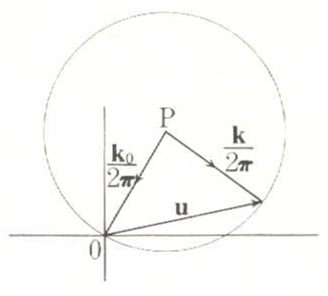
\includegraphics[height=6cm]{./images/ewald-sphere.jpg}
 \caption{ewald-sphere, ``top'' view, taken from \cite[109]{cowley_diffraction_1981}}
\end{figure}

\begin{figure}[h!]\label{LEED}
 \centering
 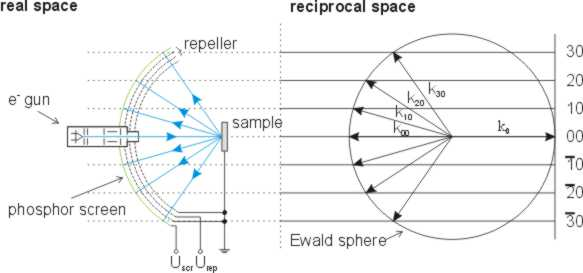
\includegraphics[height=6cm]{./images/ThreeGridLeed.jpg}
 \caption{ewald-sphere, ``side'' view, taken from \cite{threegridleed.jpg_2015}}
\end{figure}

For electrons with energies of \SI{0.04}{\eV} the diameter of the ewald sphere will be \SI{50}{\per \angstrom} in reciprocal space f. On this sphere only a small region of radius \SI{5}{\per \angstrom} will contain the small angle scattered waves of LEED.

\paragraph{Structure factor}\index{LEED!Structure factor}
Consider a function that describes the atomic positions in real space $\phi(\vec r)$. Let it be integrable, when one defines the Fourier transform such that 
\begin{equation}\label{eq:structure_factor}
\phi(\vec k)=\int_{\vec r} \phi(\vec r)e^{-i\vec k \vec r}d\vec r 
\end{equation}
If one chooses $\phi(\vec r)$ to resemble the form of the scatter partners as well - like $\phi(\vec r)=f(\vec r)\circ \sum_{j=1}^N\delta(r-R_j)$ where $R_j$ are the atom positions in real space and $f(r)$ describes the form of the atom. $\circ$ shall represent the convolution product, i.e. $FT(\phi(\vec r))=\phi(\vec k)=f(\vec k)\cdot \sum_{j=1}^N e^{-i\vec k \vec R_j}$ As the intensity $I(\vec k)\varpropto |\phi(\vec k)|^2$
$$\langle I(\vec k) \rangle \varpropto 
\langle |\phi(\vec k)|^2 \rangle =
\langle |f(\vec k)|^2 \left( \sum_{m=1}^N e^{-i\vec k \vec R_m} \right) \left( \sum_{n=1}^N e^{i\vec k \vec R_n}
\right) \rangle=|f(\vec k)|^2 \underbrace{\langle \left( \sum_{m,n=1}^N e^{i\vec k (\vec R_n-\vec R_m)} \right) \rangle }_{S(\vec k)}$$

One can calculate different structure factors for different lattices. As used crystals are fcc lattices, their basis set $R_j$ is 
$$ \vec{R}_0 = \vec{0} \quad
 \vec{R}_1 = (a/2)(\vec{a_1} + \vec{a_2})\quad
 \vec{R}_2 = (a/2)(\vec{a_2} + \vec{a_3})\quad
 \vec{R}_3 = (a/2)(\vec{a_1} + \vec{a_3})$$ with indices given by (1/2,1/2,0), (0,1/2,1/2), (1/2,0,1/2).

Following the definition of \eqref{eq:structure_factor} above, one gains an relation of $\vec {k}=(h,k,l)^T$ that describes the structure factor. Exchanged $\vec k$ with $\vec q$ in the calculation for clarity.
\begin{align*}
S_{\vec{q}} &=  f \left[ e^{-i\vec{q}\cdot\vec{0}} + e^{-i\vec{q}\cdot(a/2)(\vec{a_1} + \vec{a_2})} + e^{-i\vec{q}\cdot(a/2)(\vec{a_2} + \vec{a_3})} + e^{-i\vec{q}\cdot(a/2)(\vec{a_1} + \vec{a_3})} \right] \\
&= f \left[ 1 + (-1)^{h + k} + (-1)^{k + l} + (-1)^{h + l} \right] \\
&=  \begin{cases} 4f &\mbox{h,k,l all even or all odd}\\
                  0 &\mbox{mixed parity} \end{cases}
\end{align*}
This means, that only diffractions with $S_{\vec q}\neq 0$ contribute to the diffraction pattern. For fcc lattices, only sets of all even or all odd (h,k,l) create the pattern. 

For bcc its $$ \vec{R}_0 = \vec{0} \quad
 \vec{R}_1 = (a/2)(\vec{a_1} + \vec{a_2}+ \vec{a_2})$$ and thus 
 $$(h,k,l)=\begin{cases} 2f &\mbox{h,k,l all even}\\
                  0 &\mbox{h,k,l all odd} \end{cases}$$ due to the different basis.

In general, the structure factor is a imaginary quantity. It has the form $S(\vec k)=F_{hkl}e^{-i\alpha_{hkl}}$. $F_{hkl}$ describes the super-positioned amplitudes, while $\alpha_{hkl}$ is the phase of the resulting scattered wave. One can think of it, like having the same atoms on a crystal plane (hkl) scattering the incoming wave, with the same amplitude for each equal atom and the same phase. Now consider a parallel plane (hkl) with the same plane distance but occupied with another set of the same atoms. Since these planes are parallel Braggs law is fulfilled, the incident wave gets scattered but with a phase shift that depends on the two plane's separation. The structure factor takes these planes into account and adds the two scattered waves into one. Since these planes are created by the basis of the crystal, one just needs to know the single atom's distance to the initial plane (arbitrarily chosen atom, mostly $\vec 0$) to calculate the structure factor. If atoms are not the same, i.e. their scattered amplitude is not the same, the structure factor adapts with different $f_i$'s for different atomic species. Further reading into computational efforts and such can be done in ref. \cite{van_hove_surface_1979}.

Further reading into determining overlayer distances and structure of S on Ni can be found here \cite{demuth_small_1973,duke_structure_1973,andersson_surface_1972}
\paragraph{Temperature correction}\index{Debye-Waller factor}
Corrections have to be made if thermal motion is included. A solid with temperature $T$ has some kinetic energy which makes the atoms able to oscillate around their central position $R_j$. If one replaces $R_j$ in the calculation above with some time dependend value $\vec r_i(t)=\vec r_{i,0}+\vec u_i(t)$, with fast changing function $u(t)$ describing the dislocation from the ideal position, one yields:
$$ \langle S(\vec q) \rangle =\sum_{i}f_{i}\,\langle\exp\left[i\,\vec{q}\cdot\left(\vec{r}_{i.0}+\vec{u}_{i}(t)\right)\right]\rangle=\sum_{i}f_{i}\,\exp\left[i\,\vec{q}\cdot\vec{r}_{i.0}\right]\,\langle\exp\left[i\,\vec{q}\cdot\vec{u}_{i}(t)\right]\rangle $$
Expanding the exponential function to terms $\leq 2^{nd}$ order 
$\langle \exp\left[i\,\vec{q}\cdot\vec{u}_{i}(t)\right] \rangle \approx 1+i\,\langle \vec{q}\cdot\vec{u}_{i}(t)\rangle-\frac{1}{2}\langle\left(\vec{q}\cdot\vec{u}_{i}(t)\right)^2\rangle$ where the first term equals zero because $\langle \vec{u}_i(t)\rangle=0$ (vibration around center).

$$\langle \left(\vec{q}\cdot\vec{u}_{i}(t)\right)^2 \rangle=|\vec{q}|^{2}\,\langle|\vec{u}_{i}(t)|^2\rangle \,\langle\cos^{2}\theta\rangle$$ The time avarage 
$$ \langle \cos^{2}\theta \rangle=\frac{\int_{0}^{2\pi}\mathrm{d}\phi\int_{0}^{\pi}\mathrm{d}\theta\,\sin\theta\cos^{2}\theta}{\int_{0}^{2\pi}\mathrm{d}\phi\int_{0}^{\pi}\mathrm{d}\theta\,\sin\theta}=\frac{1}{3} $$ inserted into the expansion results in
$$\langle \exp\left[i\,\vec{q}\cdot\vec{u}_{i}(t)\right]\rangle \approx1-\frac{1}{6}\,|\vec{q}|^{2}\,\langle|\vec{u}_{i}(t)|^2\rangle \approx \exp\left[-\frac{1}{6}\,|\vec{q}|^{2}\,\langle|\vec{u}_{i}(t)|^2\rangle \right]$$
Put it in the definition of $\langle S(\vec q) \rangle$ results in
$$\langle S(\vec q) \rangle =\underbrace{\sum_i f_{i}\,\exp\left[i\,\vec{q}\cdot\vec{r}_{i,0}\right]}_{S_0(\vec q)}\,\exp\left[-\frac{1}{6}\,|\vec{q}|^{2}\,\langle|\vec{u}_{i}(t)|^2 \rangle \right]$$
Time averaging the intensity yields $$\langle I \rangle \propto \langle S(\vec q)\rangle^2 =S_0^2(\vec q)\,\exp\left[-\frac{1}{3}\,|\vec{q}|^{2}\,\langle|\vec{u}|^2\rangle \right]=I_{0}\underbrace{\exp\left[-\frac{1}{3}\,|\vec{q}|^{2}\,\langle|\vec{u}|^2\rangle \right]}_{DWF}$$
\begin{itemize}
 \item This means the higher the amplitude of displacements (higher T), the weaker the overall intensity of the spots. This is consistent with the idea that the higher the temperature, the lower the coherence between two areas. This reduces the intensity.
 \item The DWF reduces the intensity for peaks $|\vec q|>0$ so that peaks with high $|\vec q|$ have less intensity than those with small $|\vec q|$. For initial reading and detailed calculations see \cite{debye_interferenz_1913}.
\end{itemize}
The attenuation of intensity from the DWF can be used to investigate oscillating dislocations of surface atoms. As one would expect the kinetic energy from a vibration with force constant D (harmonic oscillator) to be $D\langle u^2\rangle$, its thermal energy is $k_bT$. When now the atom faces a missing surface layer (and therefore becoming itself one) the atoms left to share energy with lie in the same plane or below. It one assumes pairwise interaction one would expect $D$ to be halfed or $\langle u^2 \rangle$ compared to a intact pair of atoms\cite[69]{woodruff_modern_1986}. Although vibrations may be accessible in LEED it is not well suited to address this question. As other studies indicate the effect of enhanced amplitudes is most dominant at the very surface and - due to the fact that LEED probes several layers - it may average $\langle u^2 \rangle$ over the first 3-5 layers.

One may look deeper into what causes scattering when electrons face atoms. The coulomb interaction is strong and electrons get scattered depending on the electron density of the atom. So if one knew both the amplitude and the phase of the scattered electrons, one could calculate the electron densities. Since the phase can not be obtained a workaround has to be chosen such that one has a relative measurement of the in- and outcoming phases. If one adds an electronically denser item (like a metal atom) in the crystal it will change the diffraction pattern and one may derive the phases from that. Same is done with molecules, where one compares an already resolved scattering pattern with the ``new'' one to track changes and calculate the phase.

Another (quantum mechanical) description can be found in \cite[341]{liuksiutov_two-dimensional_1992}.

\paragraph{Spot shapes and changes} to them are given in \cite[36]{woodruff_modern_1986}, along with a detailed error evaluation. It describes under witch condition peak splitting may occur and gives examples for peak splitting related to domain boundaries and different atomic ordering on surfaces. If the surface is made of vicinal steps (i.e. 100 steps with 111 terraces, like 532) one can see 
\begin{itemize}
 \item The lattice of the substrate (in this case the unit cell contains the step distance and height)
 \item Splitted LEED spots which arise from the kinked surface and the periodic defect step formation on the ctystal\cite[37ff]{riemann_ionic_2002}.
\end{itemize}

\paragraph{Friedel's law}\cite[93]{cowley_diffraction_1981}
Provided that for the electrons no absorption effect is important, the electron desity $\rho(\vec r)$ may be assumed to be a real function satisfying \begin{align}
F(-\vec u) &= \int \rho(\vec r) \exp{[2\pi i(-\vec u)\vec r]} d\vec r \\                                                                                                                                                      &=F^\star(\vec u)                                                                                                                                                      \end{align}
As the intensities scale with $I=|F|^2$ it follows that inversion of a crystal through a center of symmetry does not change the diffraction intensities in a kinematic (single scattering) approximation. Since the inversion of \eqref{eq:structure_factor} gives the electron density $$\rho(r)=\int F(\vec u)\exp{[-2\pi \vec u \vec r]} d\vec u$$ If the diffraction amplitudes could be measured so that $F(\vec u)$ could be derived, than $\rho (\vec r)$ can be calculated by evaluating the integral numerically. But measurement of the wave amplitudes $F(\vec  u)$ is not possible, only the intensities $FF^*$ are recorded. Thus information on the phases is lost and $\rho(\vec r)$ not calculable.

\paragraph{superstructure determination}
\underline{\ \ \ \ \ \ \ \ asd \ \ \ \ \ \ \ \ \ }
\subsection{Multiple scattering theory}See \cite[55]{woodruff_modern_1986} for concepts of modeling, \cite{van_hove_surface_1979} for explaining the calculations.

The incident beam of coherent (waves have equal phases) electrons are diffracted under the fulfillment of Laue's law to result in coherent radiation on the LEED screen. Above only single scattering event were taken into account but the interaction of electrons and solid is much more pronounced than for example for X-rays. So electrons scattered once will be able to scatter a second or third time, following again Laue's law. This implies scattering on the very same oriented crystal planes. Then the phases are uniquely defined and the waves amplitudes are added. This is referred to as ``dynamical'' scattering. So if the crystal has some impurities, grain-boundaries and such, scattered electrons will be attenuated. Multiple scattering therefore gives an indication on the purity of the crystal itself. On the other hand, if atomic ordering does not extend over areas required for defined scattering the relative phases of each ordered crystal domain will add up randomly and their amplitudes are added incoherently. This is referred to as ``multiple elastic scattering''.

As a comparison, the path length for X-rays to be scattered multiple times is $\approx \SI{1}{\micro \meter}$, serveral times longer for neutrons and only one or two hundert \si{\angstrom} for eletrons\cite[90]{cowley_diffraction_1981}.

\paragraph{Resolution and difficulties}
I real world experiments, there is often a spread in incoming wave momenta and the problem of focus. 
\textbf{Finite Sources - Ewald shell emergence}
For LEED witch magnetic focus, the angle of convergence may be chosen as high as \SI{E-3}{\radian}(within magnetic lenses of an tunneling electron microscope). But even within this small range of angles, the appearance of the Ewald sphere changes. If one chooses two different angles for incoming waves $\vec k_0$ the waves scatter in different directions resulting in a blurring of diffraction spots.

\paragraph{Wavelength spread}
For electrons a nearly monochromatic radiation with line widths of about $10^{-6}\lambda$ are achieveable (1981). The spread of wavelengths in the incoming beam modifies the length of the $\vec k_0$ and as a result the diffracted spot shapes change from spots to lines variing as well in orientation as in length\cite[113]{cowley_diffraction_1981}``being small and parallel to $\vec k_0$ in the limit of small scattering angles; of medium length and roughly perpendicular to $\vec k_0$ like for intermediate scattering angles and of maximum length and oppositely directed to $\vec k_0$ for scattering angles of \SI{180}{\degree}''.

Adding this effect to the finite source problem, one ends in a complicated scattering volume. Thus the relationship of the observed intensity to the function $|F(\vec q)|^2$ is only to derived by calculation from a detailed model containing the parameters of the experimental system.

For some examples of vacancy deviations, see \cite[144-151]{cowley_diffraction_1981}.
In LEED, if the size of diffraction elements are smaller than the width of the transfer function, one observes broadening in the peaks and therefore makes it able to access their size\cite[40]{liuksiutov_two-dimensional_1992}.


  \section{\textbf{X}-ray \textbf{P}hotoelectron \textbf{S}pectroscopy}
	\label{section:XPS}\index{XPS} 
\textbf{X}-Ray \textbf{p}hotoelectron \textbf{s}pectroscopy (XPS) is a tool to achieve information of the samples chemical structure.
When X-rays with sufficient energy hit metals, electrons are emitted. This effect is called photoelectric effect and was first discovered by Heinrich Hertz in 1887 through the fact that electrodes illuminated with ultraviolet light create electric sparks more easily. \cite{hertz_ueber_1887} 18 years later Albert Einstein received the Nobel Price for his discovery of the law of the photoelectric effect\cite{_nobel_2015} and a scientific explanation which Hertz was missing. The emitted electron's kinetic energy depends on the element the electron was emitted from and allows for exact identification of the atomic species on the sample.

\subsection{Theory}
\index{XPS!Physical model}As the X-rays hit and penetrate the sample surface they excite electrons and initiate core-level excitations.

For the \textbf{core-level excitation} the X-ray removes a single electron strongly bound to the core. Energy conservation due to elastic scattering of the electron out of the bulk results in the relation 
\begin{align}
%E_{kin} &= h\nu_{\textnormal{X-ray}}-E_{B}-\Phi_{\textnormal{analyzer}} \\
E_B 	&=h\nu_{\textnormal{X-ray}}-E_{kin}-\Phi_{\textnormal{analyzer}}
\end{align}
 $h\nu_{\textnormal{X-ray}}$ is the energy of the incident X-ray beam, $E_B$ the binding energy of the excited electron and $\Phi_{analyzer}$ the work function of the analyzer. The stronger the binding energy, the less energy is left for kinetic energy.


\begin{figure}\centering
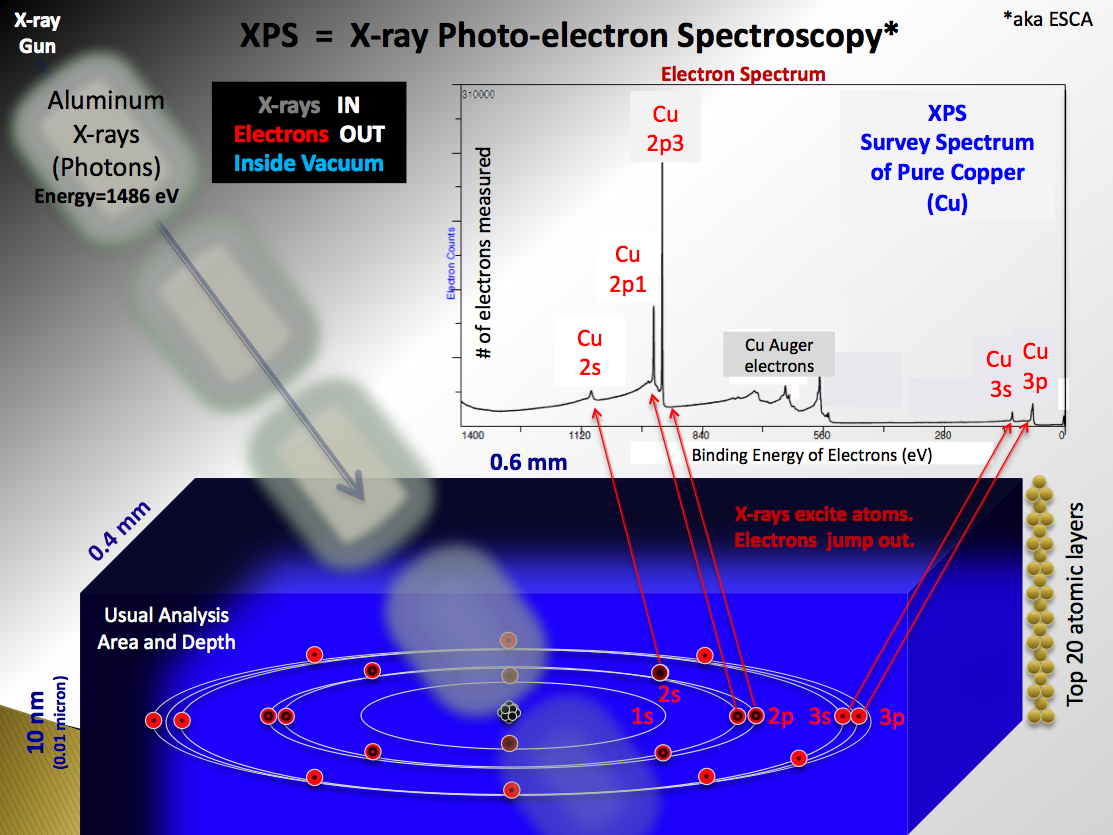
\includegraphics[width=0.7\textwidth]{./images/XPS_PHYSICS}
		\label{fig:XPS-excitation}
	\caption{Representation of a XPS process. A scheme of a X-ray gun illuminating a sample area of about \SI{0.4}{\milli \meter} $\times$ \SI{0.6}{\milli \meter} is shown. X-rays are used to excite core level electrons. Excited electrons within the first 20 layer escape the sample. After leaving the sample these show element specific signatures in their kinetic energies. A detailed analysis of the peak shift allows for identification of the chemical environment.}
	\label{fig:auger-core}
\end{figure}

\cite{zemlyanov_versatile_2018}
The \index{XPS!chemical surrounding} \textbf{chemical surrounding} of atoms changes their binding energy, making XPS an ideal tool to detect changes in chemical surrounding. Although the analysis is averaged over the area of the incident X-rays its results are very precise. This makes it possible to distinguish differently bound atoms within single atomic species and therefore gives rise to otherwise not directly observable processes like growth, intercalation, etching and binding of for example 
graphene islands on Ir(111)\cite{busse_graphene_2011-1,granas_oxygen_2012}.
The \index{XPS!binding energies} binding energies of some atomic transitions are given in \autoref{tab:XPS-intensities}.

\begin{table}\centering
 \caption{Element specific transitions and binding energies for some chosen elements as reported in \cite{wanger_handbook_1979}}
 \begin{tabular}{lll}
  Element & Ground state & $E_B$ [eV]\\ \hline 
  O & 1s & 531\\
  N & 1s & 398.1\\
  C & 1s & 285\\
  B & 1s & 189.4 \\
%  Cu & 2p $\frac{1}{2} (\frac{3}{2})$ & 953 (933) \\
%  Cu & LMM & 560-580 \\
  Cu & 3s & 123\\
  Cu & 3p $\frac{1}{2} (\frac{3}{2})$ & 77 (75)\\
 \end{tabular}
\label{tab:XPS-intensities}
\end{table}

The shape of the peaks typically resembles the line shape of the used X-rays (Gauss width $\approx 1eV$). In case of s-states $(l=0)$ (B\textit{1s}, N\textit{1s}, C\textit{1s}) the peaks are singlets. With increasing $j=l+s$, the spin-orbit (j-j) coupling introduces a 'parallel' and 'anti-parallel' nature of the spin, resulting in two different $j=\frac{1}{2}(\frac{3}{2})$ and therefore two different energies.
% The split in energy is expected to increase with the atomic number Z (for constant n,l) or as l decreases (n constant). This makes the splitting of 3p orbitals larger than that of the 3d's. 
The ratio of the two peaks is given by their degeneracy $(2j+1)$\cite[113]{Riviere_90}, so that the $\textnormal{Cu3p}\frac{3}{2}$ peak is two times larger than $\textnormal{Cu3p}\frac{1}{2}$.

\subsection{Experimental details}
The \textbf{X-ray sources} used are supplied with aluminum and magnesium anodes.
%\footnote{Other materials are available that produce various X-ray energies and line widths \index{XPS!Anode materials} \cite{_x-ray_2015}.} 
With these, electrons are accelerated with typically \SI{15}{\keV} onto the anode of choice. Most of the created radiation is made up of the principal characteristic line ($K\alpha_{1,2}$). Higher ones ($K\alpha_{3,4}$, $K\beta$) are also observed but with much lower intensities. In addition there is a continuous background called Bremsstrahlung extending up to the energy of the incident electron energy. This background is of no use for the XPS measurement and has to be subtracted in a more or less artificial way. For XPS measurements the Mg K$\alpha$ = \SI{1253.6}{\eV} and Al K$\alpha$ = \SI{1486.6}{\eV} are used situationally to shift the core level spectra with respect to substrate transitions (Auger transitions) at constant kinetic energy.

The more atoms of a specific kind are present, the larger the signal gets. Therefore the signal intensity resembles the amount of atoms on the topmost surface layers($\approx \SI{10}{\nm}$). As each irradiated atomic species has a different \textbf{cross section} for adsorption of X-rays with a certain energy they emit spectra with a different intensity. Comparing the cross section of e.g. N and B, one can see that it it roughly 4 times as large (B: \SI{6,87e3}{\barn\per atom}, N: \SI{25,82e3}{\barn\per atom}) for $\textnormal{Al} K_{\alpha}$\cite{henke_x-ray_1993}. Meaning that the signal from the N is much stronger than that of the B, although their number of atoms is equal.

\textbf{Gracing and normal emission} are two operational modes in XPS. The maximum information depth in XPS measurements is mainly limited by the escape length of excited core level electrons ($\approx \SI{10}{\nano \meter}$) for electrons. The mean free path of electrons with energy E in a solid is approximated by $\lambda = \frac{143}{E^2} + 0.054 \sqrt{E} \stackrel{E=\SI{1}{\kilo \eV}}{\approx} \SI{1.7}{\nano \meter}$.\cite{Seah_Quantitative_1979} This is much smaller than the penetration depth of X-Rays which are in the order of \SI{10}{\nano \meter}. An increasing angle between sample and detector increases the path the electrons have to travel through the bulk to reach the analyzer. Because the mean free path of the electrons stays the same, a longer route in the bulk attenuates the signal of lower lying substrate atoms. Electrons leaving the surface adsorbate are not attenuated and gain in signal strength relative to the bulk atoms.

Some supporting measurements are done in gracing emission to increase an otherwise small signal of an surface adsorbate but are not shown in this work.

The spectra used in this work are recorded without monochromator. Experiments are done at two different XPS setups. (1) The RT-STM/XPS (2) The NIM-XPS chamber.  

\subsection{Limitations}
\paragraph{Beam damage}
Since the X-Rays carry considerable energy other effects than the excitation of core electrons are possible. Especially for long integration times of the analyzer (for elements with little cross section or little surface coverage) the amount of deposited energy results in unwanted side reactions on the surface. It is possible to trigger a change in the chemical surrounding of the investigated element, causing chemical shifts that are not present in the pristine sample and change the XPS spectrum over time.

\paragraph{Space averaging technique}
XPS is a space averaging technique. First the X-Ray beam has an inherent width, the analysis area can't be chosen arbitrarily small. Second, X-Rays do excite electrons not only directly within the illuminated area, but penetrate the bulk and cause a cascade of transitions in the sample. The resulting information is always a mix between surface adsorbates and bulk elements.
  \section{Surfaces and ad-layers}
     \subsection{Crystal facets}
        Single crystals show a nicely ordered, clean surface - two properties important for reliable and reproducible experiments. We have chosen both silver and copper as bulk crystalline substrates. Both form fcc lattices and their surface termination can be fixed by precise cutting along a symmetry plane of choice. For the course of this thesis, experiments are conducted mainly on (111) and (100) terminated surfaces.
%\footnote{See \cite{riemann_ionic_2002} and appendix \fullref{appendix:crystal-facets} for another examples of vicinal metal surfaces (531), (532), (221), (311), (211).} Commercially available single crystals guarantee a high precision in facet orientation and purity (99.999 \%) \cite{mateck}. 
Remaining contaminations 
%in copper (Ag: \SI{0.8}{ppm}, Pb: \SI{0.3}{ppm}, Bi: \SI{0.8}{ppm}) and silver (Cu: \SI{2}{ppm}, Fe: \SI{2}{ppm}, Au: \SI{0.8}{ppm}, Ni: \SI{0.8}{ppm}) 
are removed by repeated sputter\footnote{$U_{accel}=$\SIrange{800}{1000}{\volt}, $T_{sample}\approx \SI{300}{\kelvin}$} and anneal cycles\footnote{Cu: $T_{sample}=\SI{750}{\celsius}$, Ag: $T_{sample}=\SI{450}{\celsius}$, Au\textbackslash Mica: $T_{sample}= \underline{\textbf{get value: 450?}}$} in UHV. Typical cool down temperatures $\leq 5 \frac{K}{s}$ result in a smooth, atomically flat surface with large terrace size. 

The lattice constants at room temperatures for \underline{\textbf{cite!}} Cu(\SI{3,61}{\angstrom}), Ag(\SI{4,09}{\angstrom}) and Au(\SI{4,07}{\angstrom}) are related to the environment temperatures by their expansion coefficients.
Coefficients of \SI{16,5e-6}{\per \kelvin}(Cu), \SI{18,9e-6}{\per \kelvin}(Ag) and \SI{14,2e-6}{\per \kelvin}(Au) make the substrate lattice shrink by $\approx \SI{0,5}{\percent}$ when it is cooled down from RT to low temperature measurement conditions in STM/AFM (\SIrange{5}{7}{\kelvin}). While rather negligible for bulk materials that are not heated and cooled over larger temperature ranges, the small change in substrate lattice size may introduce strain in grown ad layers since these are grown via CVD typically at elevated temperatures and may have thermal expansion coefficients with opposite sign (\textcolor{red}{\textbf{Give expansion coefficient for \textit{h}-BN}}).\cite{farwick_zum_hagen_structure_2016}

%\begin{table}
%\centering \index{Crystal:lattice constants}
%\caption{Inter atomic distances for Cu and Ag with respect to different surface termination. $a$ denotes the lattice constant and $\beta= \SI{60}{\deg}$ the angle within the (111) unit cell}
%  \begin{tabular}{ccccc}
%& Lattice constant a [\SI{}{\angstrom}] & Nearest neighbors [\SI{}{\angstrom}] & diagonal [\SI{}{\angstrom}]\\ \hline 
%\multicolumn{2}{c}{fcc(100)} & $\frac{\sqrt{2}a}{2}$ & a \\
%  Cu	 	& 3.61	& 2.55 | 2.55 & 3.61  \\
%  Ag		& 4.09	& 2.89 | 2.89 & 4.09 \\ \hline 
%\multicolumn{2}{c}{fcc(111)} & $\frac{\sqrt{2}a}{2} \ <110>$ & $\sqrt{2}a\sin(\frac{\beta}{2})$ | $\sqrt{2}a\cos(\frac{\beta}{2})$\\
%Cu 		& 3.61	& 2.55 | 2.55	& 2.55 | 4.42 \\
%Ag		& 4.09	& 2.89 | 2.89	& 2.89 | 5.01 \\ \hline
%%
%%\multicolumn{2}{c}{fcc(110)} & $\frac{\sqrt{2}a}{2}$ | a & $\sqrt{\frac{3}{2}}a$\\
%%  Cu	 	& 3.61	& 2.55 | 3.61	& 4.42 \\
%%  Ag		& 4.09	& 2.89 | 4.09	& 5.00 \\ \hline 
% \end{tabular}
%\end{table}

\begin{figure}\centering
	\subfigure[(111)]{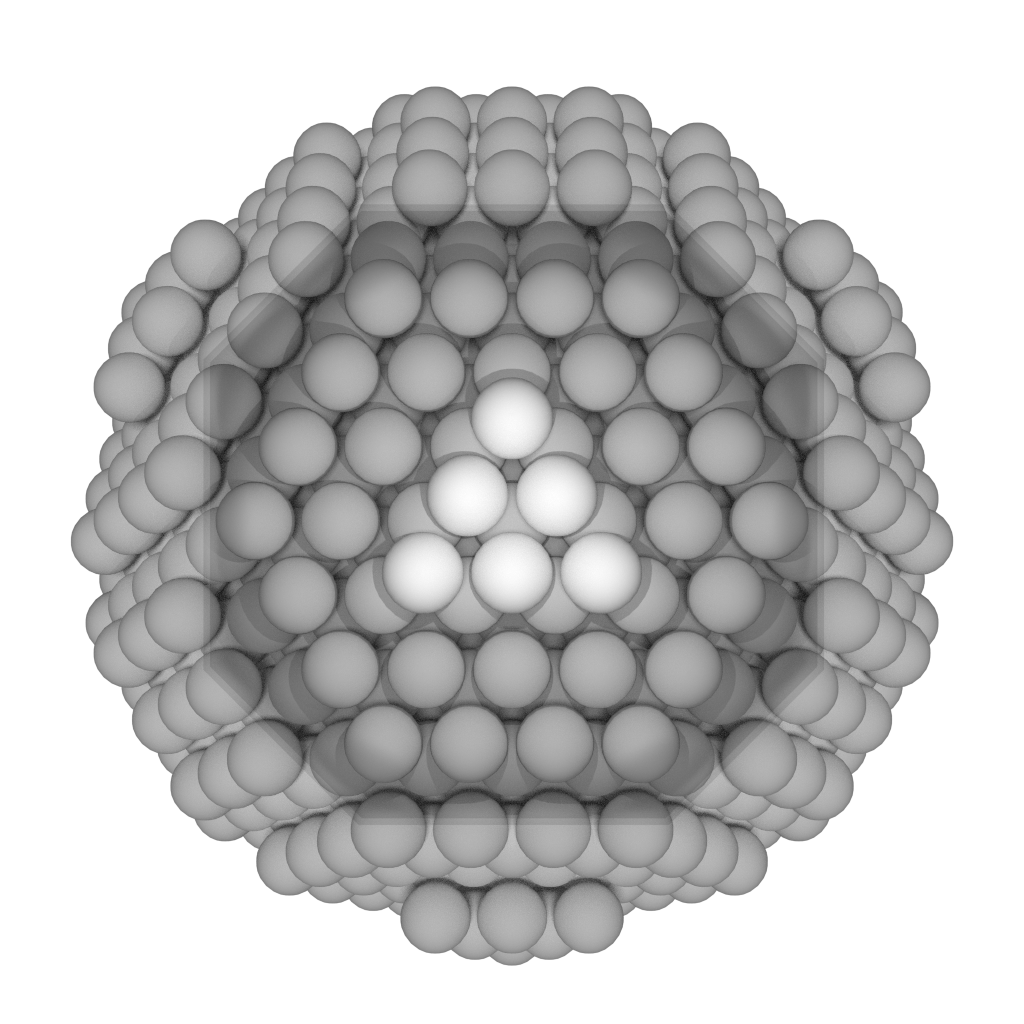
\includegraphics[width=0.3\textwidth]{./images/fcc-111-persp}} \quad
	\subfigure[(100)]{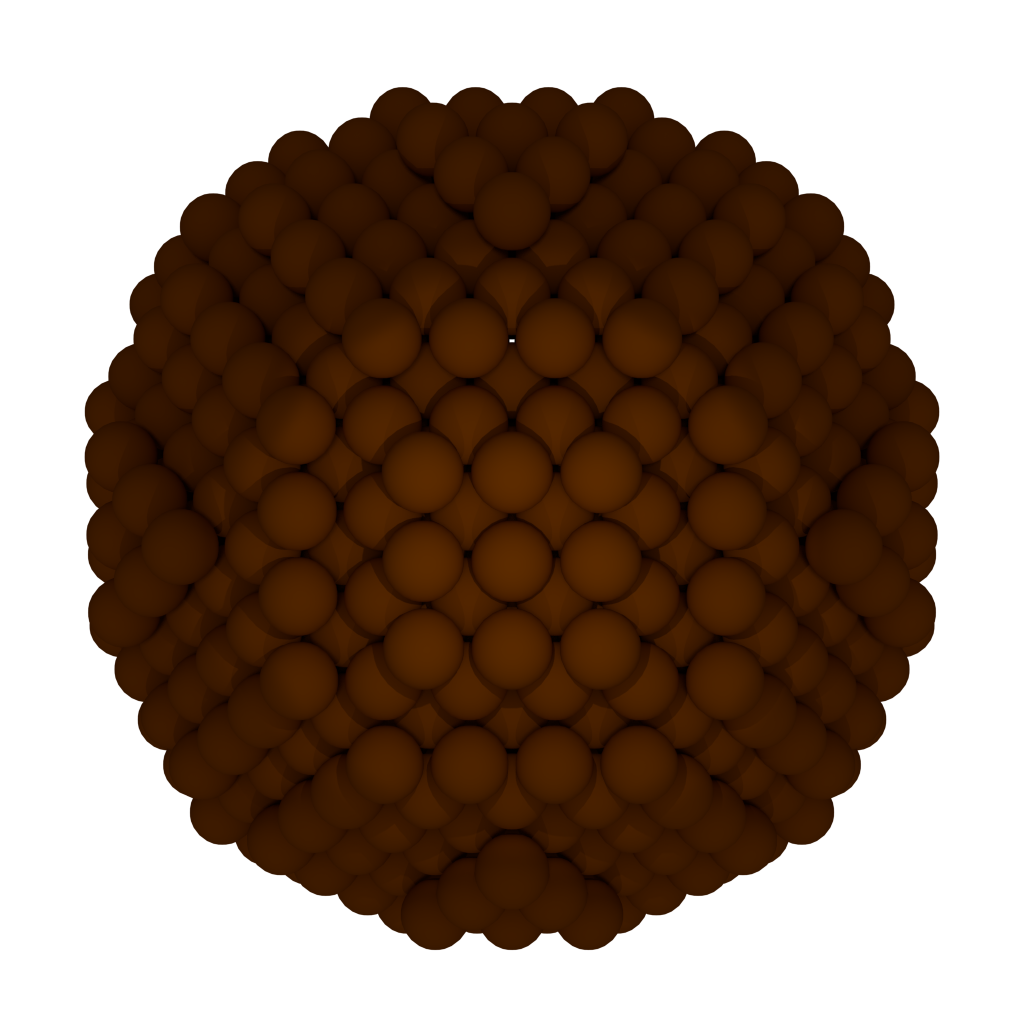
\includegraphics[width=0.3\textwidth]{./images/fcc-100-persp}}
%	\subfigure[(110)]{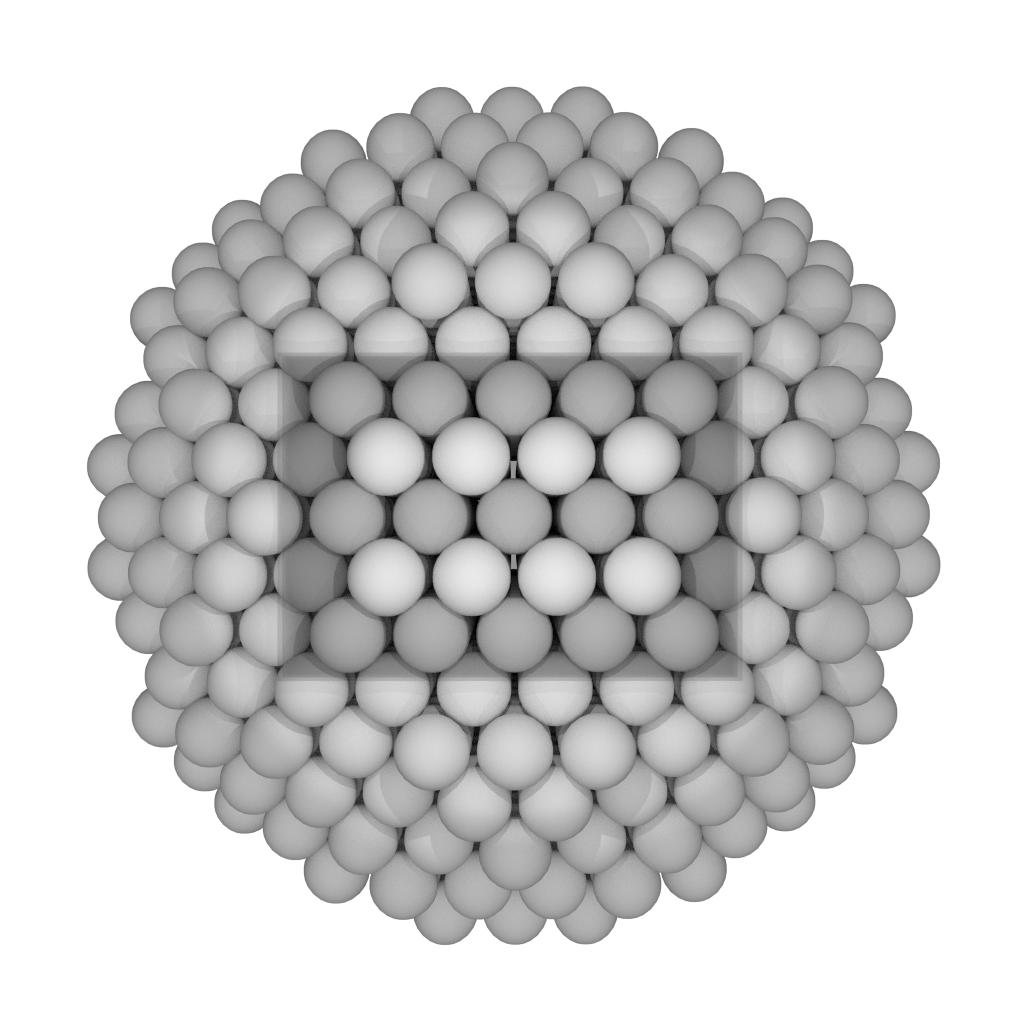
\includegraphics[width=0.3\textwidth]{./images/fcc-110-persp}}
	\caption{Identical crystalline balls in fcc lattice configuration. The surface termination is determined by the direction of the intersecting plane (parallel to the paper plane) relative to the lattice and forms (111) and (100) surfaces.}
	\label{fig:crystal-termination}
\end{figure}

The surface free energy increases from the (111) surface with increasing angle of the (hkl) planes of interest with $$\cos(\phi)=\frac{h+k+l}{\sqrt{3(h^2+k^2+l^2)}}$$ \cite{jian-min_calculation_2004}. Thus, the (111) surface is the one with lowest energy, followed by (110) and (100). For polycrystalline foils it is expected to observe the lowest energy facet more often than the less favorable (110) and (100) facet.

Due to the fact that dislocation lines move within the crystal in a well defined manner, one can determine the crystals orientation when dislocation lines and step edges show on the surface.

\textcolor{red}{\textbf{
For fcc crystals the orientation of dislocation lines occurs in the {111} plane in $<110>$ direction. Its Burgers vector is $\frac{a}{2}[110]$\cite{_dislocation-theory}. \underline{ADD INFO	FOR 100!!!}
Dense packed rows in fcc(111) are the following directions: $<\bar 1 01>$, $<01\bar 1>$, $<1\bar 1 0>$. The diagonals are found in the $<\bar 1 \bar 1 2>$ and $<1\bar 2 1>$ directions. \underline{ADD INFO	FOR 100!!!}
}}
 
 \subsection{Polycrystalline copper foils}
 
  As was mentioned before, clean, highly ordered surfaces are desirable to perform experiments on. In case a systems order and functionality does not heavily depend on the substrates crystalline properties, single crystals loose most of their unique selling point. Instead of choosing a expensive bulk single crystal, thin copper foils can catch up in production environments. The mass produced foils, although pure ($\geq \SI{99.999}{\percent}$), were never meant to be atomically flat and show considerable height variation.

\begin{wrapfigure}{O}{4cm}\centering
	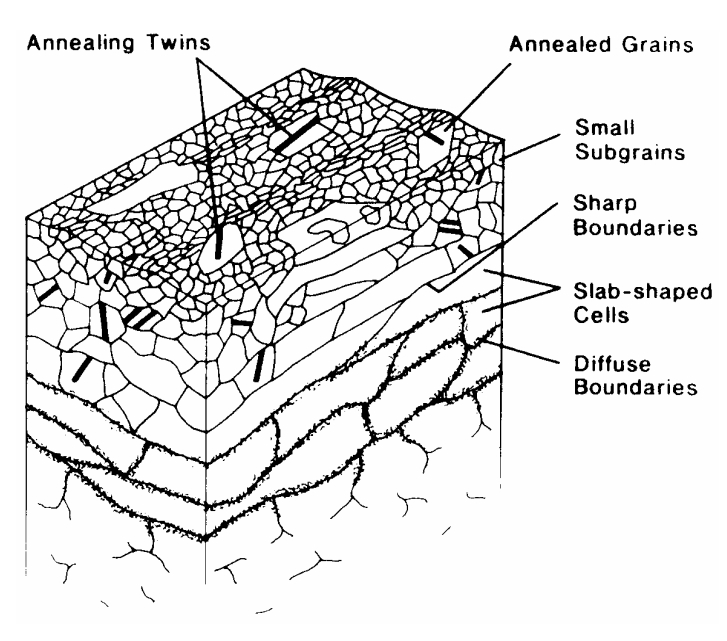
\includegraphics[height=40mm]{./images/grain-structure-copper-foil}
	\caption{Sketched bulk structure of a OFHC copper foil after abrasion with P1200 silicon carbide paper. Adopted from \cite{turley_nature_1981}}
	\label{fig:copper-foil-grains}
\end{wrapfigure}

 A representation of a mechanically polished copper surface can be seen in \autoref{fig:copper-foil-grains}. Here the layered structure is apparent and shows different sizes of grains. Small subgrains constitute the uppermost layers, while deeper lying layers consist of larger grains with grain boundaries becoming more and more diffuse with increasing distance to the surface. 
 
To overcome the limitation of small grain size and heavily corrugated surface, etching of the copper foil is performed as described in \autoref{sec:etching}.
     \subsection{Surface states}
		In the discussion of surface states, one generally distinguishes between Shockley states[5] and Tamm states,[6] named after the American physicist William Shockley and the Russian physicist Igor Tamm. However there is no real physical distinction between the two terms, only the mathematical approach in describing surface states is different. 

\paragraph{Shockley states - Electron gas approximation} from wikipedia article \\
Historically, surface states that arise as solutions to the Schr\"odinger equation
in the framework of the nearly free electron approximation for clean and ideal surfaces, are called Shockley states. Shockley states are thus states that arise due to the change in the electron potential associated solely with the crystal termination. This approach is suited to describe normal metals and some narrow gap semiconductors. Figures 1 and 2 are examples of Shockley states, derived using the nearly free electron approximation.''

\paragraph{Tamm states - Tight binding approximation (LCAO)} from wikipedia article \\
Surface states that are calculated in the framework of a tight-binding model are often called Tamm states. In the tight binding approach, the electronic wave functions are usually expressed as linear combinations of atomic orbitals (LCAO). In contrast to the nearly free electron model used to describe the Shockley states, the Tamm states are suitable to describe also transition metals and wide gap semiconductors.

\paragraph{Extrinsic surface states} from wikipedia article \\
Surface states originating from clean and well ordered surfaces are usually called intrinsic. These states include states originating from reconstructed surfaces, where the two-dimensional translational symmetry gives rise to the band structure in the k space of the surface.

Extrinsic surface states are usually defined as states not originating from a clean and well ordered surface. Surfaces that match the category extrinsic are :
\begin{itemize}
 \item Surfaces with defects, where the translational symmetry of the surface is broken.
 \item Surfaces with adsorbates
 \item Interfaces between solid and liquid phases.
 \item Interfaces between two material such as a semiconductor-oxide or semiconductor-metal interfaces
\end{itemize}
Generally, extrinsic surface states cannot easily be characterized in terms of their chemical, physical or structural properties.

%The \index{Kondo effect} \textbf{Kondo effect} also plays a role when looking at scattering of electrons on - in this special case - magnetic impurities. For further reading one is advised to read \cite{kouwenhoven_revival_2001} and citations within.
     \subsection{Geometric alteration of ad-layers -- moire}
		The properties of various moir\'e superstructure are well described in literature and Hermann gives a comprehensive overview in his paper \cite{hermann_periodic_2012}. One can conclude the following: \label{section:moire}

If lattice constants are equal like in the case of a graphene bilayer, the needed lattice mismatch occurs due to a rotation of the two layers. A moir\'e is always present if an over layer shows a lattice mismatch with respect to the substrate. 

For \textbf{isotropically scaled over layers} (refer to figure \ref{fig:moire-pattern-scaled}) one can calculate the scaling factor $$p=\frac{R^{'}_{O1}}{R_{O1}}$$ which gives the size of the over layer lattice in units of the substrate lattice. The moir\'e pattern shows the same Bravais lattice type than the substrate\cite[10]{hermann_periodic_2012}. If moir\'e and ad layer lattice are aligned ($\alpha=0$\textdegree) the direction of moir\'e and substrate is aligned. If the over layer is isotropically scaled and not rotated, the period of the moir\'e calculates to $$a_{moir\'e}=\underbrace{\frac{p}{|p-1|}}_{\kappa}a_{substrate}$$. With $a_{moir\'e}$ and $a_{substrate}$ are experimentally available, the ad layer lattice can be calculated with high precision (usually one order of magnitude more accurate than direction measurement of its period).

For a \textbf{scaled and rotated over layer} (figure \ref{fig:moire-pattern-scaled-rotated}, the angle between substrate and moir\'e ($\gamma$[rad]) scales with the angle between over layer and substrate ($\alpha$[rad]) as $\alpha=(1-p)\gamma$.

For rotated and isotropically scaled over layers, one can determine the $\alpha$ and $p$ from experimental observables $\gamma$(moir\'e angle to substrate) and $\kappa$(scaling factor) through relations $ \tan(\alpha)=\frac{sin(\gamma)}{cos(\gamma)+\kappa}\qquad p=\frac{\kappa}{\sqrt{1+\kappa^2+2\kappa cos(\gamma)}}$


\begin{wrapfigure}{l}{4cm} \centering
	\subfigure[Isotropically scaled and aligned overlayer (gr/Pt(111): $p = 0.89$)]{
		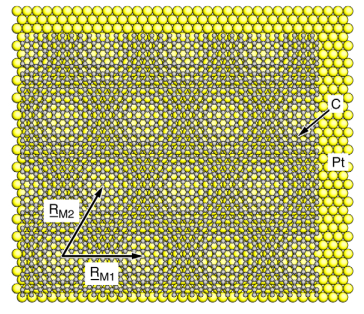
\includegraphics[width=0.25\textwidth]{./images/moire-scaled}%
		\label{fig:moire-pattern-scaled}
	}
	\subfigure[Isotropically scaled overlayer with rotation of \SI{5.4}{\degree} (gr/\textit{h}-BN: $p = 0.98$)]{
		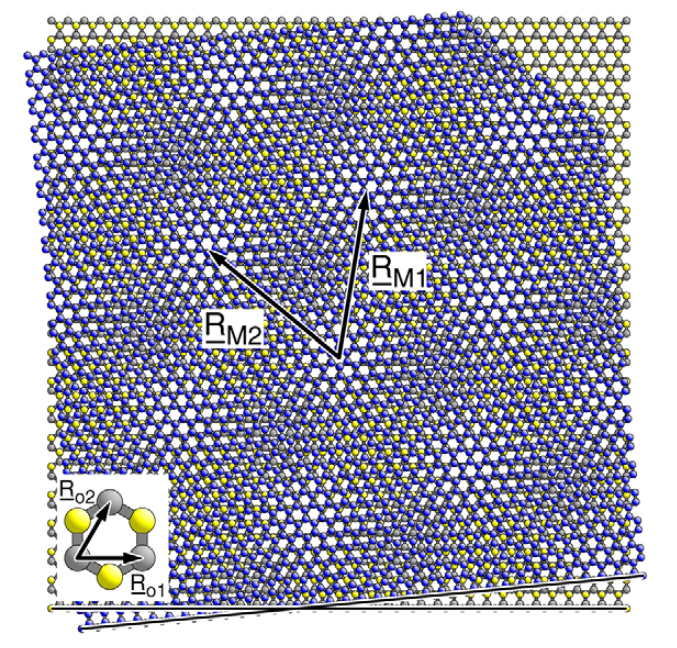
\includegraphics[width=0.25\textwidth]{./images/moire-scaled-rotated}%
		\label{fig:moire-pattern-scaled-rotated}
	}
	%	\subfigure[Isotropically scaled, alligned layer overgrowing a step edge (gr/Ir(111): $p = 0.91$)]{
	%		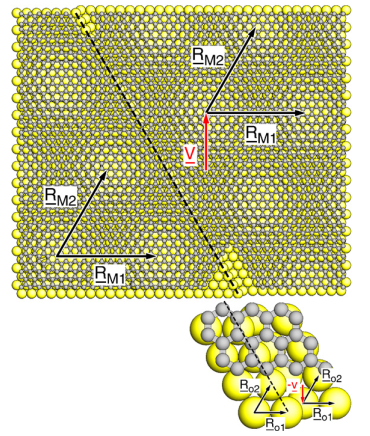
\includegraphics[width=0.25\textwidth]{./images/moire-scaled-step-edge}%
	%		\label{fig:moire-pattern-scaled-step-edge}
	%	}
	\caption{Adopted from \cite{hermann_periodic_2012}}
	\label{fig:moire-pattern}
\end{wrapfigure}\\

When a scaled over layers over grows a step edge, the moir\'e pattern is altered. While period and orientation remain the same, a lateral shift in the superstructure is observed that interrupts the regular pattern and shifts subsequent moir\'e features by a vector $\vec{V}$.

\begin{figure} \centering
	\subfigure[DFT simulation of \textit{h}-BN on Ir(111). The moir\'e unit cell as well as regions where B and N atoms occupy high-symmetry positions w.r.t. the Ir lattice are indicated. The change in adsorption height is caused by the changing registry of substrate (Ir) and ad layer atoms (B,N).  Adopted from \cite{schulz_epitaxial_2014}]{
		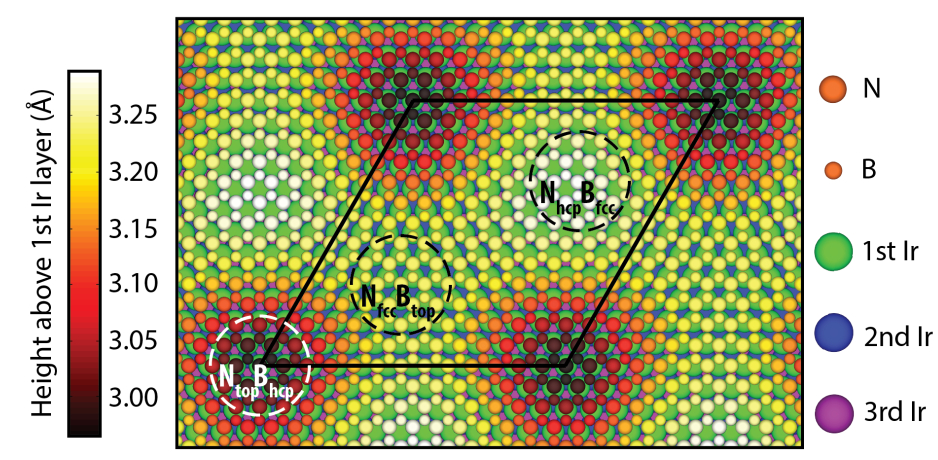
\includegraphics[width=0.5\textwidth]{./images/h-BN_Ir-moire}%
		\label{fig:h-BN-Ir-moire-DFT}
	} \quad
	\subfigure[\textbf{STM image of h-BN grown with CVD on Ir(111)}]{
		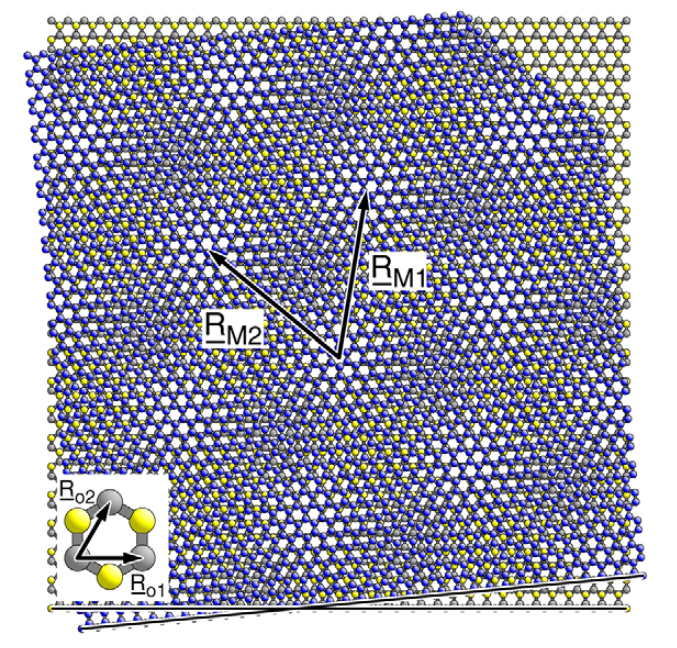
\includegraphics[width=0.25\textwidth]{./images/moire-scaled-rotated}%
		\label{fig:h-BN-Ir-moire-STM}
	}
	\caption{DTF calculation and STM images of \textit{h}-BN/Ir(111). While being aligned, a lattice mismatch creates a moir\'e  superstructure. It is well visible in adsorption height calculations \ref{fig:h-BN-Ir-moire-DFT} and as apparent height differences in STM images \ref{fig:h-BN-Ir-moire-STM}.}
	\label{fig:moire-DFT-TSM}
\end{figure}


\paragraph{Periodic change in work function}
A direct result of the lattice mismatch between \textit{h}-BN and substrate is the alternating registry of ad layer atoms and substrate. The periodic modulation of B/N registry to the substrate atoms results in regions of stronger and weaker interaction between \textit{h}-BN and substrate and is the reason for the nano templating effect of \textit{h}-BN on many substrates. 
In the following some resulting effects are discussed that lay the foundation for a nano patterning effect of \textit{h}-BN and its influence on the electronic structure of adsorbates.

After growth of h-BN the substrates work function in reduced [Rh: \SIrange{5.01}{3.07}{\eV} \cite{gomez_diaz_hexagonal_2013}. Therefor a dipole moment $\mu$ pointing from the the bulk to the surface is necessary \cite{roman_periodic_2013}, rather likely created by a negative charge transfer from the bulk into the ad layer.

\paragraph{\textit{h}-BN}
{% tex broke the page here!!!!
	\parfillskip=0pt
	\parskip=0pt
	\par}

Free standing \textit{h}-BN is investigated with \textit{ab-initio} calculations \cite{han_effects_2014,mortazavi_investigation_2012,topsakal_first-principles_2009,peng_mechanical_2012}. Together with experiments \cite{paszkowicz_lattice_2002} a crystal lattice constant of $a_{\textit{h}-BN, RT}=\SI{2.504}{\angstrom} $is derived. Depending on the substrates used, different lattice mismatches can be achieved as listed in \autoref{tab:h-BN-mismatch}. While substrates exist where the lattice constant are virtually identical ($\Delta \approx \leq \SI{1}{\percent}$), other substrates like Ag(111) show considerable deviations.

While a first report in 2004 \cite{corso_boron_2004}, pointed to the formation of a complicated two layer structure, later experiments \cite{roth_chemical_2013, li_grain_2015} including ours \cite{joshi_boron_2012, schwarz_corrugation_2017} and others  \textit{h}-BN/Cu(111) proposed a single layer of B \& N atoms in a regular hexagonal lattice. It evolved as well investigated system to perform experiments on. It could be shown that after CVD growth it adsorbs on Cu(111) as a flat layer. Due to its  lattice mismatch, "hill" regions  (corresponding to a $N_{top}B_{fcc}$ registry) and "valleys" (corresponding to a $N_{fcc}B_{hcp}$ registry) are formed. In these regions the work function is altered in opposite directions. While larger at the hill/pore regions, the work function reduces continuously to its lowest value in the valley/wire regions\footnote{Please note that the notation is not uniform throughout the literature. Sometimes hills are referred to as pores and valley regions are denoted as wire regions.}. 

With changing work function, a lateral electronic field emerges, pointing from \underline{\qquad \qquad}. It can be used to trap adsorbates with dipole moment along the field lines. This was shown for FePc and pentacene molecules on a graphene/Ru(0001) substrate. Here FePc molecules adsorp first on regions with high lateral dipole along top-fcc direction, followed by regions with lower lateral dipole. Pentacene molecules are trapped along the top-fcc direction \cite{zhang_assembly_2011}. This general adsorption mechanism is applicable for other systems with periodic modulation of the work function. \autoref{fig:ig:h-bn-cu-wf} depicts the work function change measured  with STM (Field emission resonances) indicating a similar modulation of the work function. In this theses TPB molecules (\autoref{section:TBP} and helicene molecules in \autoref{section:helicene} are used as sample molecules for specific adsorption site or orientation alignment.
\begin{wrapfigure}{r}{5cm}\centering
	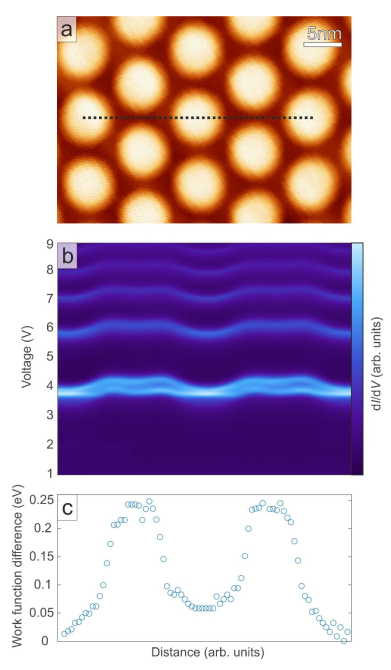
\includegraphics[width=5cm]{./images/h-BN-Cu(111)-wf-change}
	\caption{Work function variation along \textit{h}-BN/Cu(111) moir\'e. (a) STM image showing the \textit{h}-BN moir\'e with a periodicity of 8.4 nm. Scan parameter: $U_b= 4.0 V, I_t= 40 pA$. (b)	Field emission resonances acquired along the black dotted line in a) revealing a variation of the peak positions. (c) Work  function  differences  between bright  (“hill”/pore)  and  dark  (“valley”/wire)  regions obtained  from  the  dI/dV curves  of  the  field emission  resonances  displayed  in  b). Adopted from \cite{schwarz_corrugation_2017}}
	\label{fig:h-bn-cu-wf}
\end{wrapfigure}
\begin{table}\centering
\caption{Lattice mismatches between \textit{h}-BN and several transition metal surfaces. The mismatch is given to describe the relative size of the h-BN layer compared to the substrate, e.g. negative values indicate a larger lattice constant in the substrate bulk.}

	\begin{tabular}{ccc}
	Substrate 	& Mismatch [\%] \\ \hline
	Ni(111)		& \SI{+0.4}{\percent} \\
	Cu(111)		& \SI{-1.9}{\percent} \\	
	Rh(111)		& \SI{-7}{\percent} \\	
	Pd(111)		& \SI{-9}{\percent} \\
	Ag(111)		& \SI{-13}{\percent} \\

\end{tabular}
\label{tab:h-BN-mismatch}
\end{table}

As mentioned in \autoref{section:moire} the orientation of the moir\'e superstructure is determined by its rotation alone, while its period is determined by lattice mismatch, too. This results in a variety of moir\'e superstructure orientations and periods.




  \section{Used molecules}
    \label{chapter:used-molecules}
The following molecules have been used to conduct experiments. Images show the molecules in an orthographic projection. We will utilize porphyrine derivatives (\autoref{section:TBP}), functionalized pyrene molecules (\autoref{section:pyrene}), helicene species (\autoref{section:helicene}) and coronene (w\/o central borazine functionalization, see \autoref{section:HBC}).

All the depicted molecules are modeled in Hyperchem\cite{_hyperchemtm_1111} and calculated for optimized geometry with the AM1+ method. Afterwards their positions are exported and remodeled in blender. Note that this does not change their geometry. It is only for better control of the output (faster and more accurate model building especially in 3D) and for aesthetic reasons.

%%%%%%%%%%%%%%%%%%%%%%%%%%%%%%%%%%%%%%%%%%%%%%%%%%%%%%%%%%%%%%%%%%%%%%%%%%%%%%%%%%%%%%%%%%%
%%%%%%%%%%%%%%%%%%%%%%%%%%%%%%%%%%%	pyrenes   %%%%%%%%%%%%%%%%%%%%%%%%%%%%%%%%%%%%%%%%%
\subsection{Pyrene: Pyridilethynyl functionalized pyrenes}
\label{sec:pyrene}\index{molecules!Pyrene}
\begin{itemize}
	\item[tetra-pyrene:] 1,3,6,8-Tetra(4-Pyridylethynyl)pyrene
	\item[cis-pyrene:] 1,8-Bis(4-Pyridylethynyl)pyrene
	\item[trans-pyrene:] 1,6-Bis(4-Pyridylethynyl)pyrene
\end{itemize}

\begin{figure}[h!]
	\begin{center}
		\subfigure[Tetra-configuration]{
			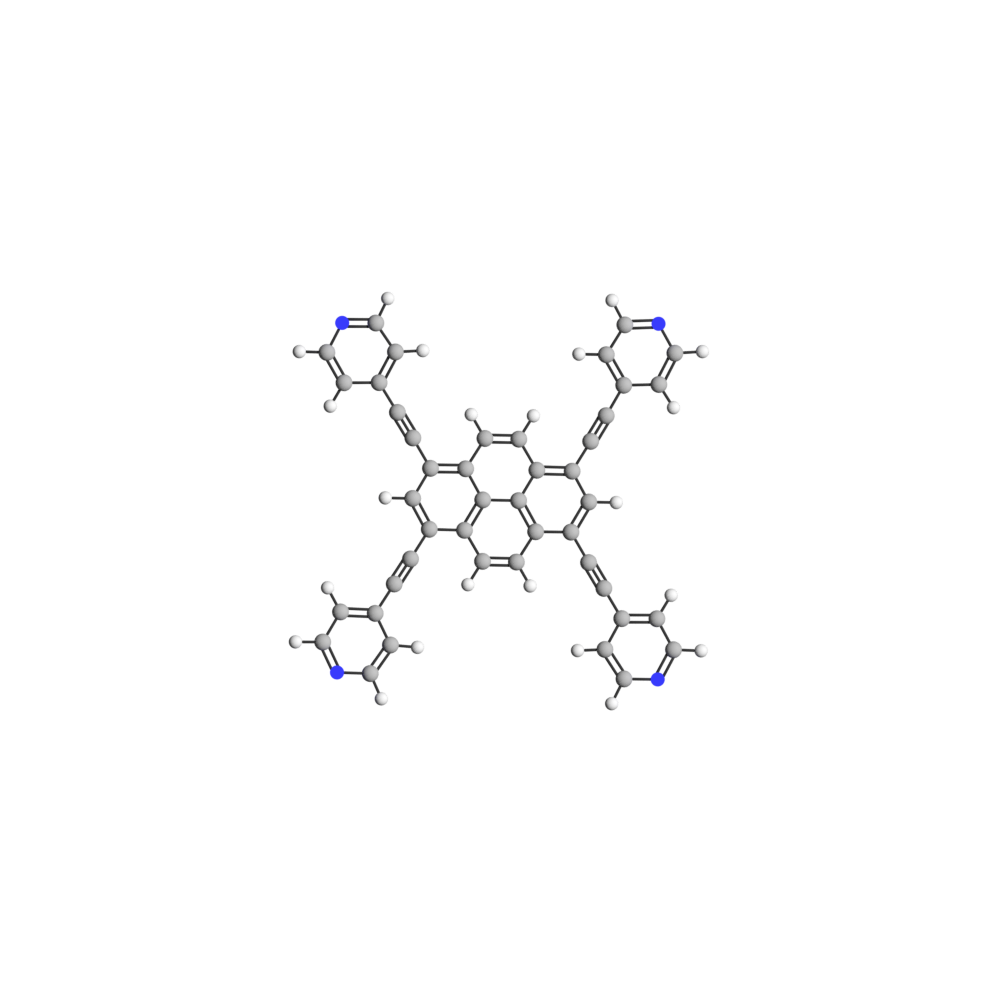
\includegraphics[width=0.3\textwidth]{./images/molecules/pyrene-tetra}
			\label{fig:pyrene-tetra}
		} 
		\subfigure[Trans-configuration]{
			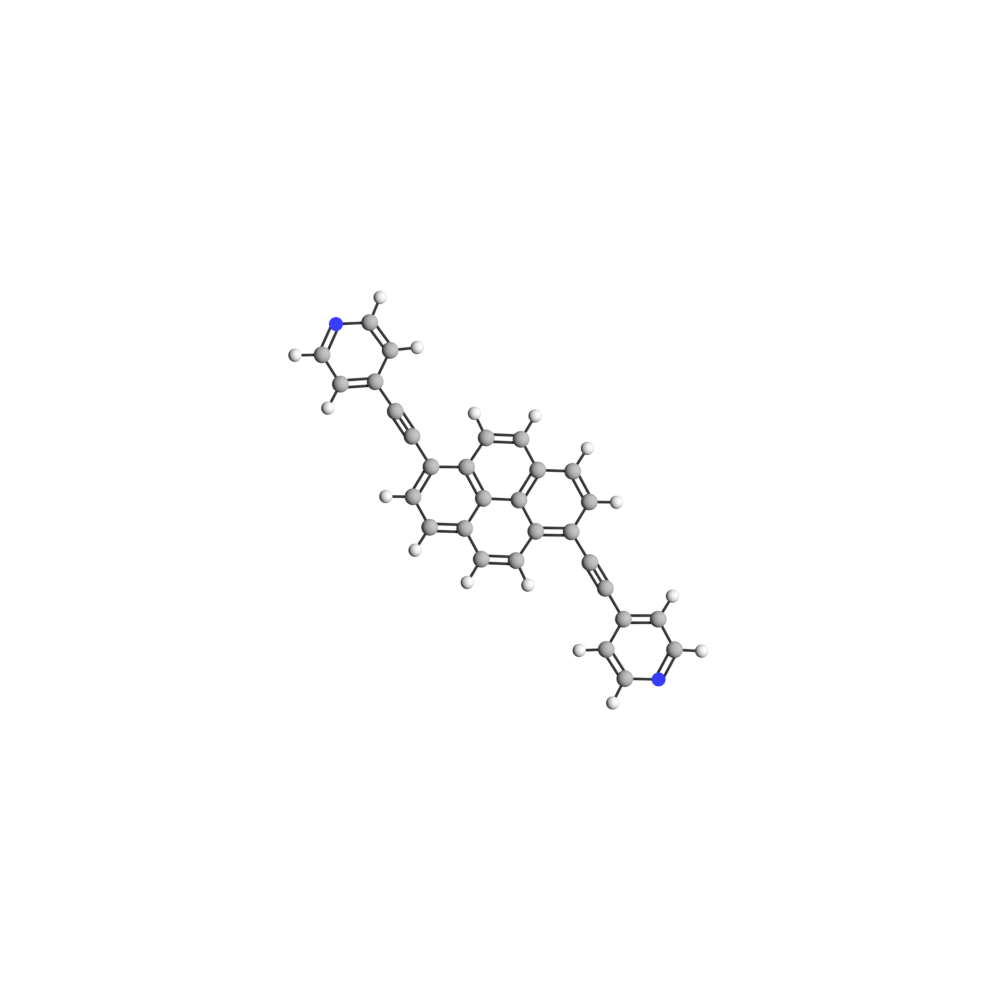
\includegraphics[width=0.3\textwidth]{./images/molecules/pyrene-trans}
			\label{fig:pyrene-trans}
		} 
		\subfigure[Cis-configuration]{
			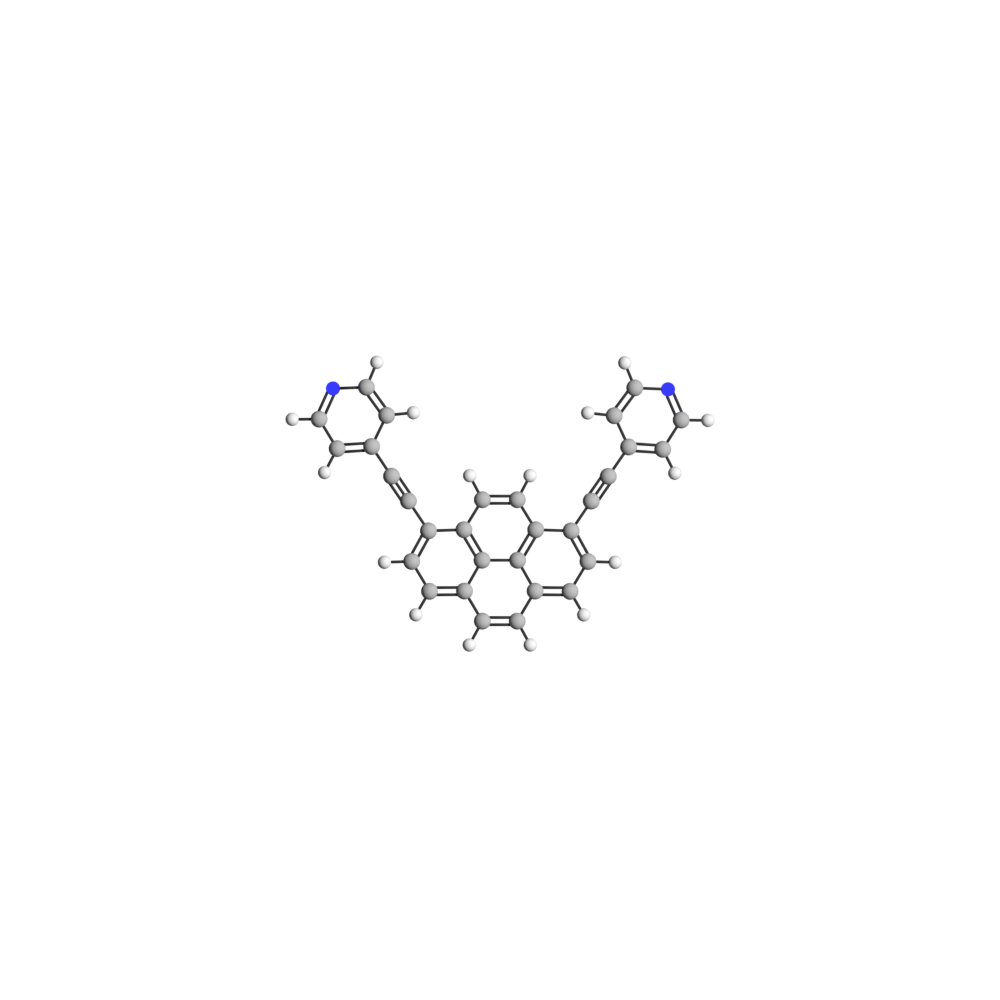
\includegraphics[width=0.3\textwidth]{./images/molecules/pyrene-cis}
			\label{fig:pyrene-cis}
		}
	\end{center}
	\caption{Pyridyl-Pyrene molecules in trans- \subref{fig:pyrene-trans} and cis- \subref{fig:pyrene-cis} and tetra- \subref{fig:pyrene-tetra} configuration}
	\label{fig:pyrene}
\end{figure}

Pyrene molecules, first investigated in 1973 \cite{khan_electronic_1973}, are 4 ortho-fused carbon rings to result in a rhombic structure. As many other $\pi$ conjugated systems they show interesting optoelectronic properties \cite{Crawford_experimental_2011, Lee_enhanced_2012, Feng_functionalization_2016, Maeda_alkynylpyrenes_2006, Kurata_donor_2017} and their assembly was investigated \cite{pham_self-assembly_2014, matena_aggregation_2010, della_pia_anomalous_2014, pham_comparing_2016}. Here they are used to investigate the influence of the number and position of functional groups on these properties. The very same species have been investigated on Cu(111) albeit data adsorbed on \textit{h}-BN/Cu(111) was lacking up to this point. The nano-pattering effect of the \textit{h}-BN substrate is used here to modulate the wide band gap of the species and therefor their optical properties.

\textcolor{red}{\textbf{DIPOLE / CHIRALITY / Ref section}}
%%%%%%%%%%%%%%%%%%%%%%%%%%%%%%%%%%%%%%%%%%%%%%%%%%%%%%%%%%%%%%%%%%%%%%%%%%%%%%%%%%%%%%%%%%%
%%%%%%%%%%%%%%%%%%%%%%%%%%%%%%%%%%%	HBBNC + HBC   %%%%%%%%%%%%%%%%%%%%%%%%%%%%%%%%%%%%%%%%%
\subsection{Coronene: HBBNC and HBC}
\label{sec:hbc}\index{molecules!Coronene}
\begin{itemize}
	\item[HBC:] 2,8,14-trixylyl-hexabenzocoronene	
	\item[HBBNC:] 2-8-14-trixylyl-hexaphenyl borazinocoronene
\end{itemize}

\begin{figure}[h!]\centering
\subfigure[HBC]{
	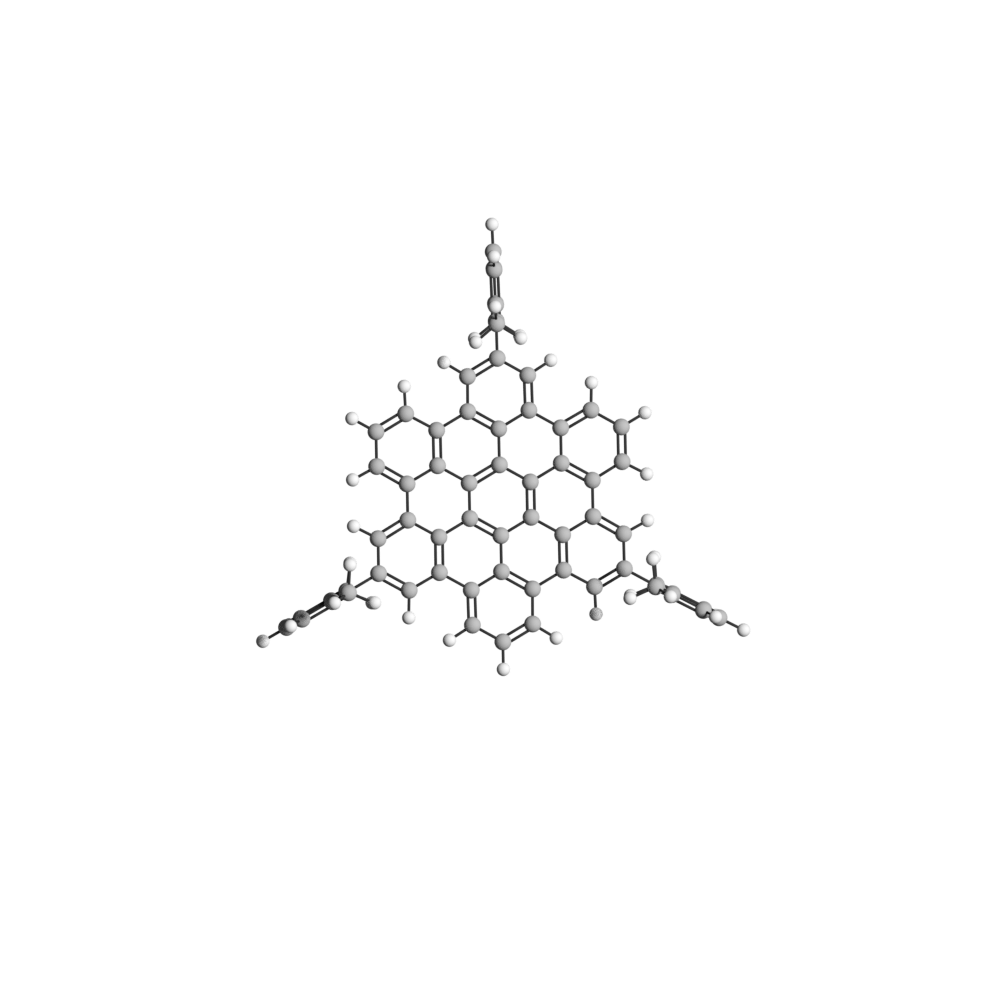
\includegraphics[width=0.3\textwidth]{./images/molecules/HBC}
	\label{fig:HBC}
} \quad
\subfigure[HBBNC]{
	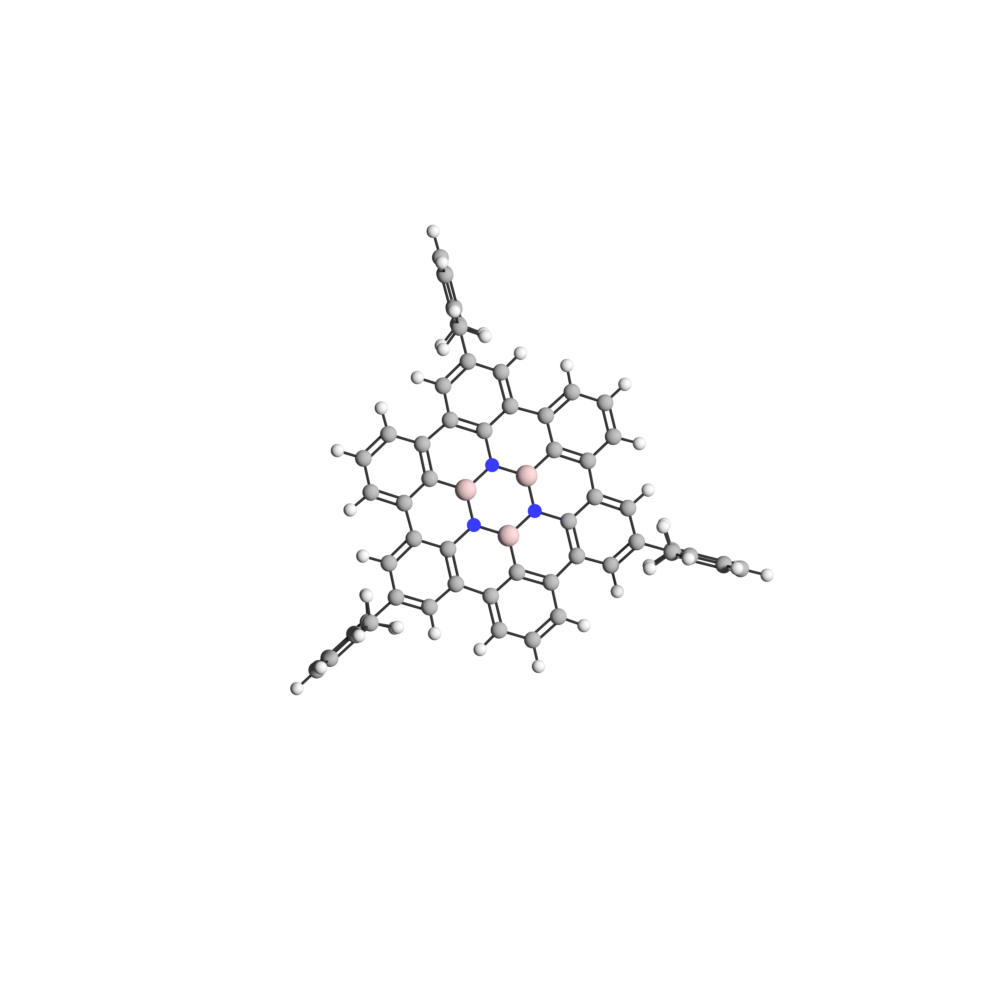
\includegraphics[width=0.3\textwidth]{./images/molecules/HBBNC}
	\label{fig:HBBNC}
}
	\caption{\subref{fig:HBC} HBC and \subref{fig:HBBNC} HBBNC}
	\label{fig:HBBNC+HBC}
\end{figure}

While in 2015\cite{Krieg_construction_2015} and 2016 \cite{Ciccullo_Quasi-Free-Standing_2016} hexy-peri-Hexabenzoborazino coronene (HBBNC) was synthesized, its bad solubility prohibited experiments. In 2017 the synthesis \cite{dosso_synthesis_2017} of a soluble, BN-doped coronene derivative by substitution of the central carbon ring was successful. 
\begin{wrapfigure}{R}{5cm}\centering
	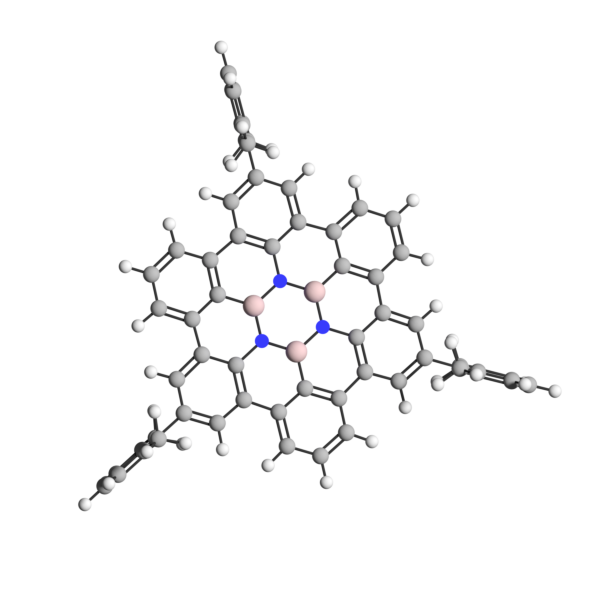
\includegraphics[angle=90,width=5cm]{./images/molecules/max-zoom/HBBNC-600}
	\caption{HBBNC}
	\label{fig:HBBNC-molecule}
\end{wrapfigure}

HBC and HBBNC are modifications of coronene. First, for both species six benzo groups are added to form a larger molecular backbone. For both species three 2,6-Dimethylphenyl groups are added to extend the molecule that now resembles a triangular footprint. While HBC features a central carbon ring, HBBNC is functionalized with a central borazine ring instead. Here the central $(BN)_3$ core is oriented to point all nitrogen atoms towards the leg functionalization.

Both species have the same number of atoms and molecular weight. The difference between both becomes apparent when electronic properties are compared (in gas phase).

The regular covalent sp2 hybridization results in an evenly distributed electron density in HBC where the central region of the molecule shows considerable depletion. Changing the central carbon ring to a borazine ring changes the electron density. Now electrons are redistributed from the coronene parts towards the central borazine ring. Because the bond between B and N shows an added ionic character the aromacity is interrupted and the extended electron pi system is altered. Comparable to the difference between graphene (perfect C-C bonds, conductor) and h-BN (Ionic B-N bonds, insulator) the band gap present for HBC is \SI{0.4}{\eV} smaller than for HBBNC, changing its optoelectronic properties. By using HBBNC the HOMO-LUMO band gap could be widened and shows blue-shifted emission properties\cite{dosso_synthesis_2017} compared to its all-carbon counterpart.

\begin{figure}[]\centering
	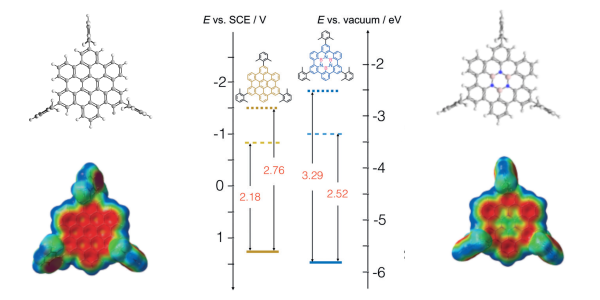
\includegraphics[width=\textwidth]{./images/dosso-combined}
	\caption{Taken from \cite{dosso_synthesis_2017}}
	\label{}
\end{figure}

The present functionalization of the coronene molecule is twofold. Di-Methylphenyl groups are added to guide the formation of self-assembled islands of the molecule on the surface. The functionalized core of the molecule is used to create an adsorption platform for polar molecules.
Investigations with STM are performed on Au(111) by \cite{Krieg_construction_2015}.

Due to the different electro negativity of the atomic species adsorption of gases in the central part can be interesting effects to look out for. Please refer to \textcolor{red}{\textbf{\autoref{section:HBC} for detailed information.}}


%%%%%%%%%%%%%%%%%%%%%%%%%%%%%%%%%%%%%%%%%%%%%%%%%%%%%%%%%%%%%%%%%%%%%%%%%%%%%%%%%%%%%%%%%%%
%%%%%%%%%%%%%%%%%%%%%%%%%%%%%%%%%%%	TPCN      %%%%%%%%%%%%%%%%%%%%%%%%%%%%%%%%%%%%%%%%%
%\subsection{TPCN}
%TPCN can be evaporated with an OMBE. Temperatures used are typically \SI{490}{\celsius}, evaporation time depends on the intended coverage. 
%\begin{itemize}
%	\item [TPCN:] Tetra[(4-cyanophenyl)-phen-4-yl] porphyrin has four arms attached to the meso-positions of the macrocycle. Each is build up from two chained phenyl rings with one end attached to the macrocycle and the other one attached to a C-N end group. Due to their flexibility, they are versatile connection segments \cite{fendt_modification_2009}.
%\end{itemize}
%
%\begin{figure}[h!]
%	\centering
%	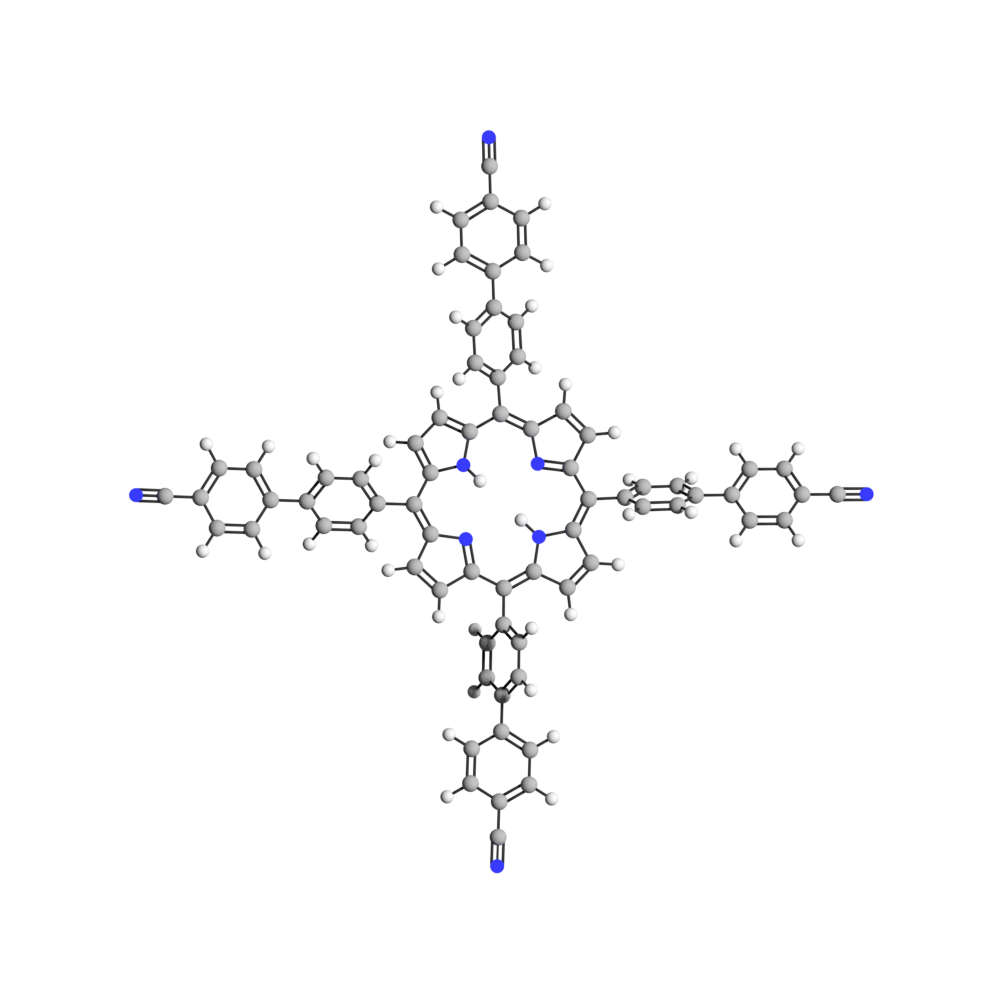
\includegraphics[width=0.3\textwidth]{./images/molecules/TPCN}
%	\caption{TPCN molecule}
%	\label{fig:TPCN}
%\end{figure}


%%%%%%%%%%%%%%%%%%%%%%%%%%%%%%%%%%%%%%%%%%%%%%%%%%%%%%%%%%%%%%%%%%%%%%%%%%%%%%%%%%%%%%%%%%%
%%%%%%%%%%%%%%%%%%%%%%%%%%%%%%%%%%%nitro-prophines%%%%%%%%%%%%%%%%%%%%%%%%%%%%%%%%%%%%%%%%%
\subsection{Porphine: [di-[tert-butyl]-phenyl)]-porphyrin derivatives}
\label{sec:TBP}\index{molecules!TBP}
\begin{itemize}
	\item[one-leg:]  	 5,10,15-Tri(3,5-di-tert-butylphenyl)-   20-(Nitrophenyl)porphyrine
	\item[two-leg cis:] 	5,10-Bis(3,5-di-tert-butylphenyl)-15,20-Bis(Nitrophenyl)porphyrine
	\item[two-leg trans:] 	5,15-Bis(3,5-di-tert-butylphenyl)-10,20-Bis(Nitrophenyl)porphyrine
\end{itemize}

\begin{figure}[h!]\centering
	\subfigure[Single functional group]{
		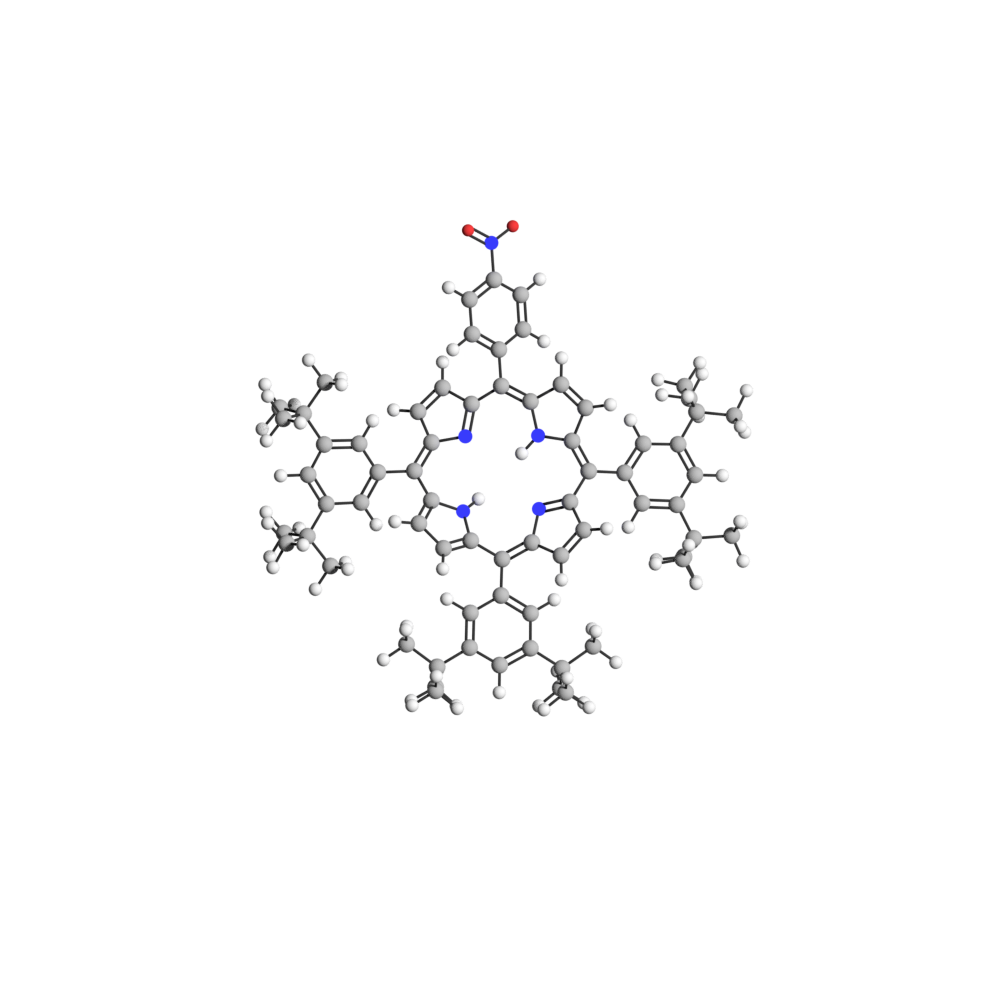
\includegraphics[angle=90, width=0.3\textwidth]{./images/molecules/TBP-single}
		\label{fig:TBP-single}
	} %
	\subfigure[Trans-configuration]{
		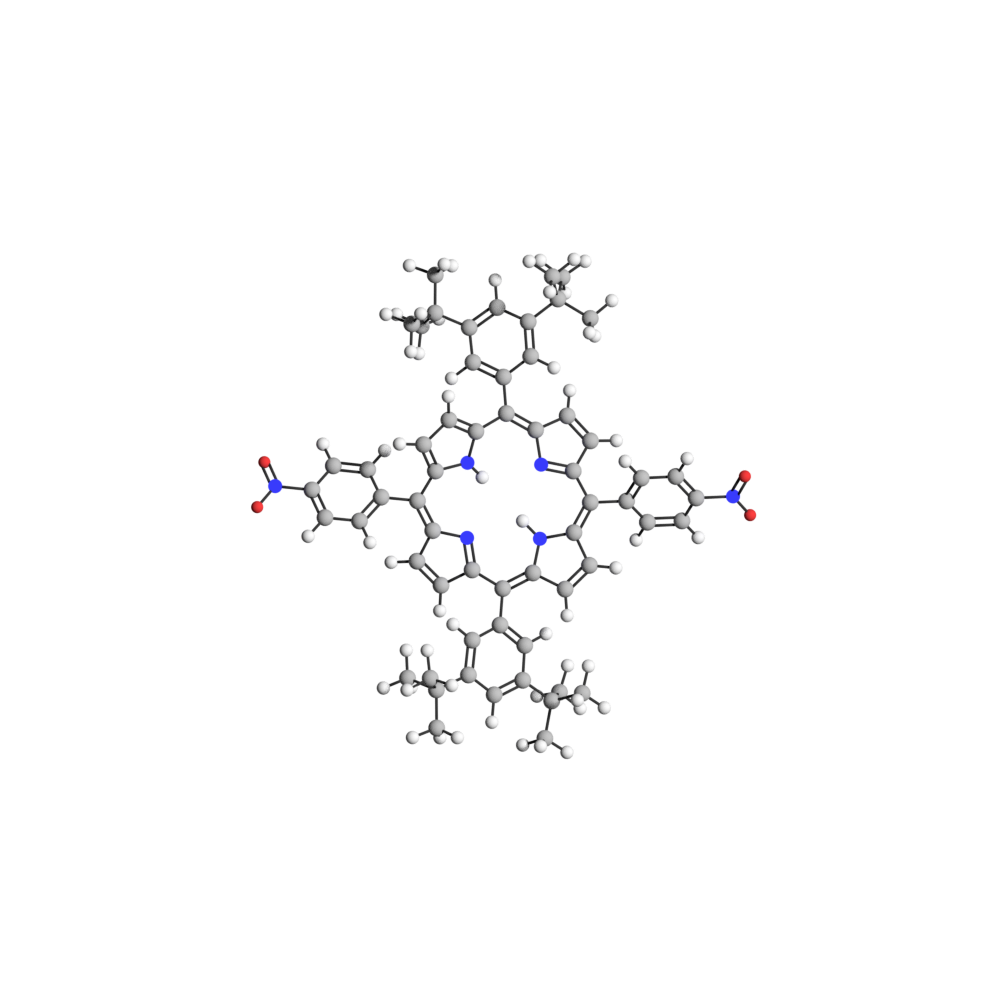
\includegraphics[angle=0, width=0.3\textwidth]{./images/molecules/TBP-trans}
		\label{fig:TBP-trans}
	} %
	\subfigure[Cis-configuration]{
		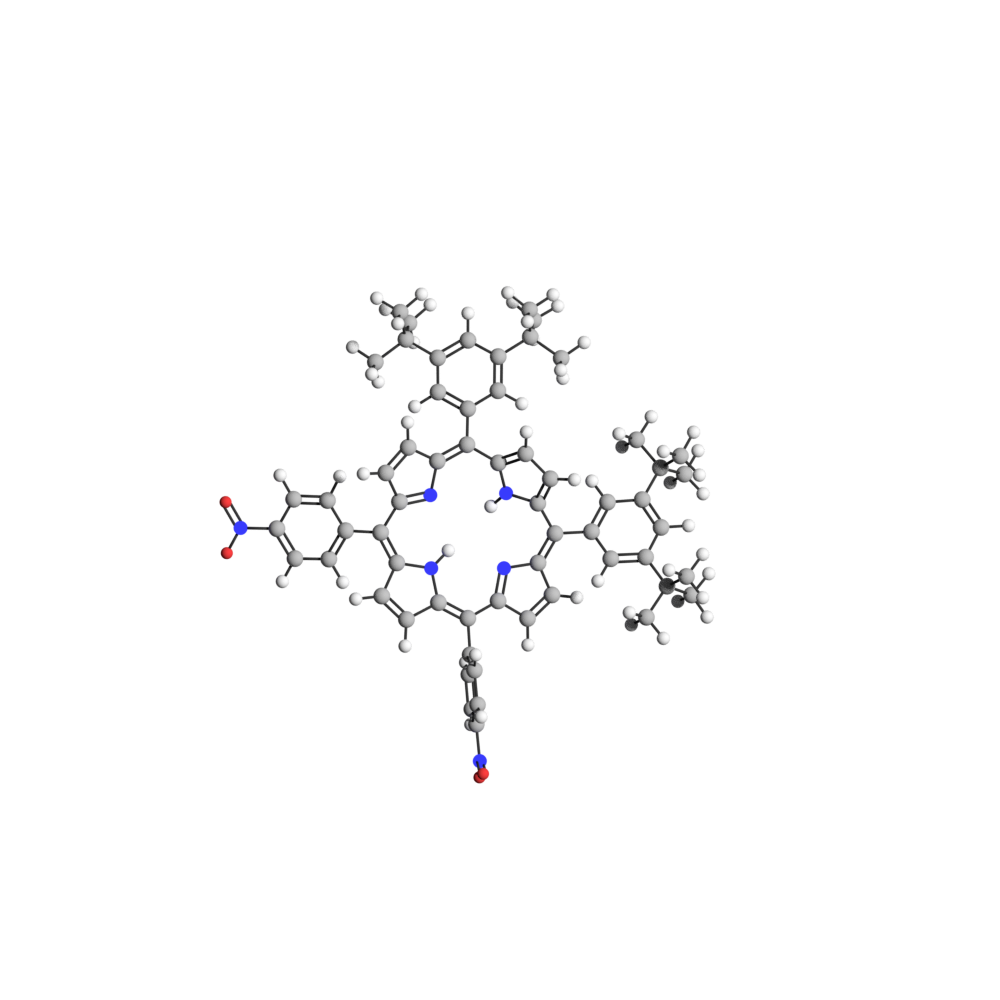
\includegraphics[angle=0, width=0.3\textwidth]{./images/molecules/TBP-cis}
		\label{fig:TBP-cis}
	} %
	\caption{Functionalized tert-butyl-phenyl-porphines. \subref{fig:TBP-single} shows a single functionalized porphine molecules. An additional function may be added in \subref{fig:TBP-cis} cis-  and \subref{fig:TBP-trans} position.}
	\label{fig:TBP}
\end{figure}	

Tetrapyrroles like porphyrins and phthalocyanines play important roles in biological systems \cite{battersby_tetrapyrroles_2000}. Both species are able to incorporate metal atoms that control the function. Not only are they interesting model systems to study interaction towards a (metallic) substrate\cite{auwarter_porphyrins_2015, auwarter_controlled_2007, diller_vacuo_2016}. Their use in metal-organic frameworks highlights the use of scientific knowledge to design "real world" sensor applications\cite{Lustig_Metal-organic_2017}. 


Tert-butyl functionals have been used in a variety of molecules \cite{moresco_conformational_2001}. Due to their bulky nature, they electronically decouple the porphyrin’s delocalized p-orbital system from the metallic surface just by lifting the molecule. They may undergo heavy conformational deformation when outer influences (like metalization of the central porphine core) act on the molecule \cite{stark_massive_2014}. Switching capabilities are well investigated \cite{loppacher_direct_2003} and it is possible to switch them with a voltage pulse through the STM tip \cite{ditze_energetics_2014}. Experiments with similar molecules investigate the heat-induced formation of 1D and 2D conglomerates on a Au(111) surface.\cite{pham_heat-induced_2015}

\begin{itemize}
	\item Free base nitrophenyl - 5,10,15 Tri [di-[tert-butyl]-phenyl)]-porphyrin \index{nitro porphin} has 3(2) di-tert-butyl-phenyl groups attached to the porphine macro cycle at the meso-positions of the molecule. The free meso-positions are occupied with nitrophenyl groups as shown in \autoref{fig:TBP-single} If more than one functional group is present, one can distinguish between trans (\autoref{fig:TBP-trans}) and cis configuration (\autoref{fig:TBP-cis}), whether the two functional groups are opposite or neighboring.
	\item The appearance of STM data is correlated to the molecular configuration according to \cite{mishra_current-driven_2015} meaning that the lobes consisting of (3,5-di-tert-butylphenyl) are imaged as bright protrusions, while the functional nitro group is imaged fainter. This holds true for cis- and trans-substituted molecules\cite{yokoyama_selective_2001}.
	\item Tert-butyl groups can rotate to form flexible legs. Interaction with the substrate results in adsorption-induced conformational changes.\cite{ecija_dynamics_2016}
\end{itemize}
Drawings for various functional groups and molecules can be found in \cite{jorgensen_salem_1973}.
\textcolor{red}{\textbf{DIPOLE, ref section}}
%%%%%%%%%%%%%%%%%%%%%%%%%%%%%%%%%%%%%%%%%%%%%%%%%%%%%%%%%%%%%%%%%%%%%%%%%%%%%%%%%%%%%%%%%%%
	%%%%%%%%%%%%%%%%%%%%%%%%%%%%%%%%%%%	helicenes %%%%%%%%%%%%%%%%%%%%%%%%%%%%%%%%%%%%%%%%%
	\subsection{Helicene: Cyano functionalization of helicenes}
	\label{sec:helicene}\index{molecules!Helicene}
	\begin{itemize}
		\item[Dicyano-dibenzo-[5]helicene]: 7,8-Bis(cyano)-Dibenzo-helicene
	\end{itemize}
	
	\begin{figure}[h!]
		\centering
		\subfigure[Top view]{
			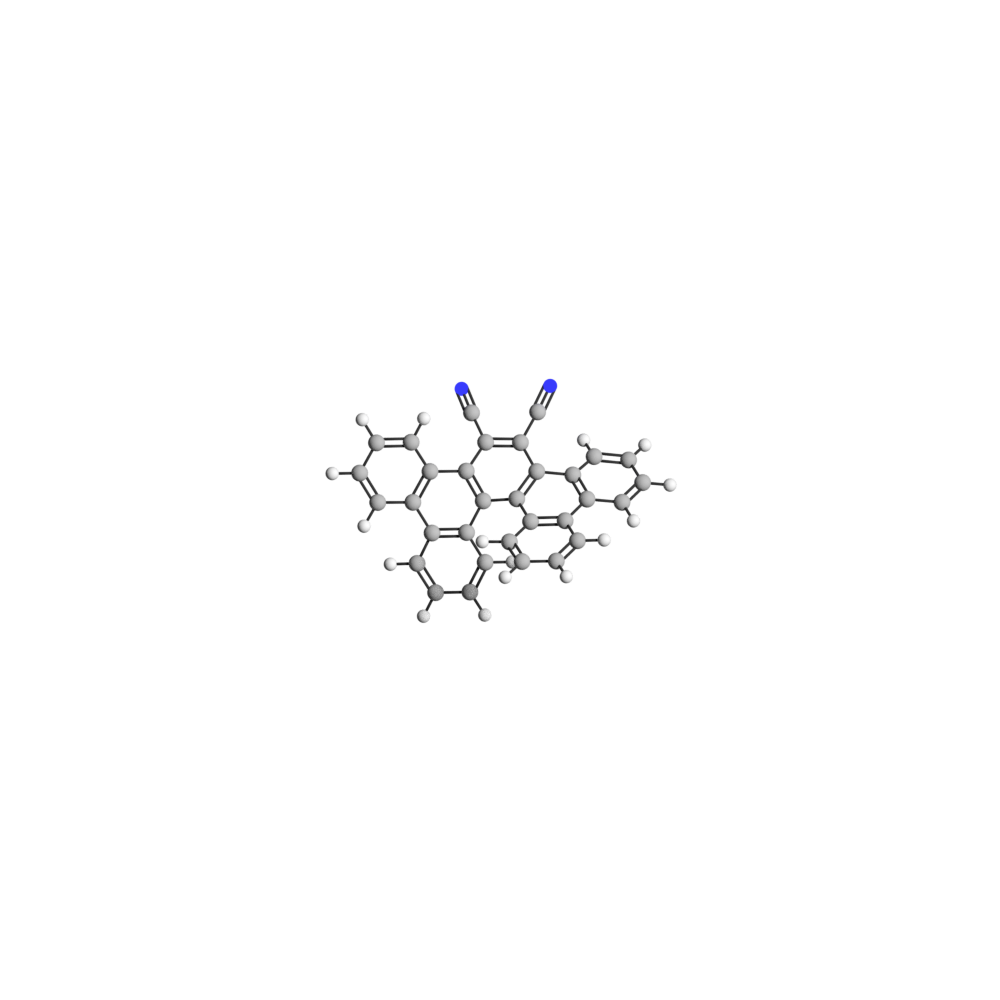
\includegraphics[width=0.3\textwidth]{./images/molecules/helicene}
			\label{fig:helicene-top}
		} \quad
		\subfigure[Side view]{
			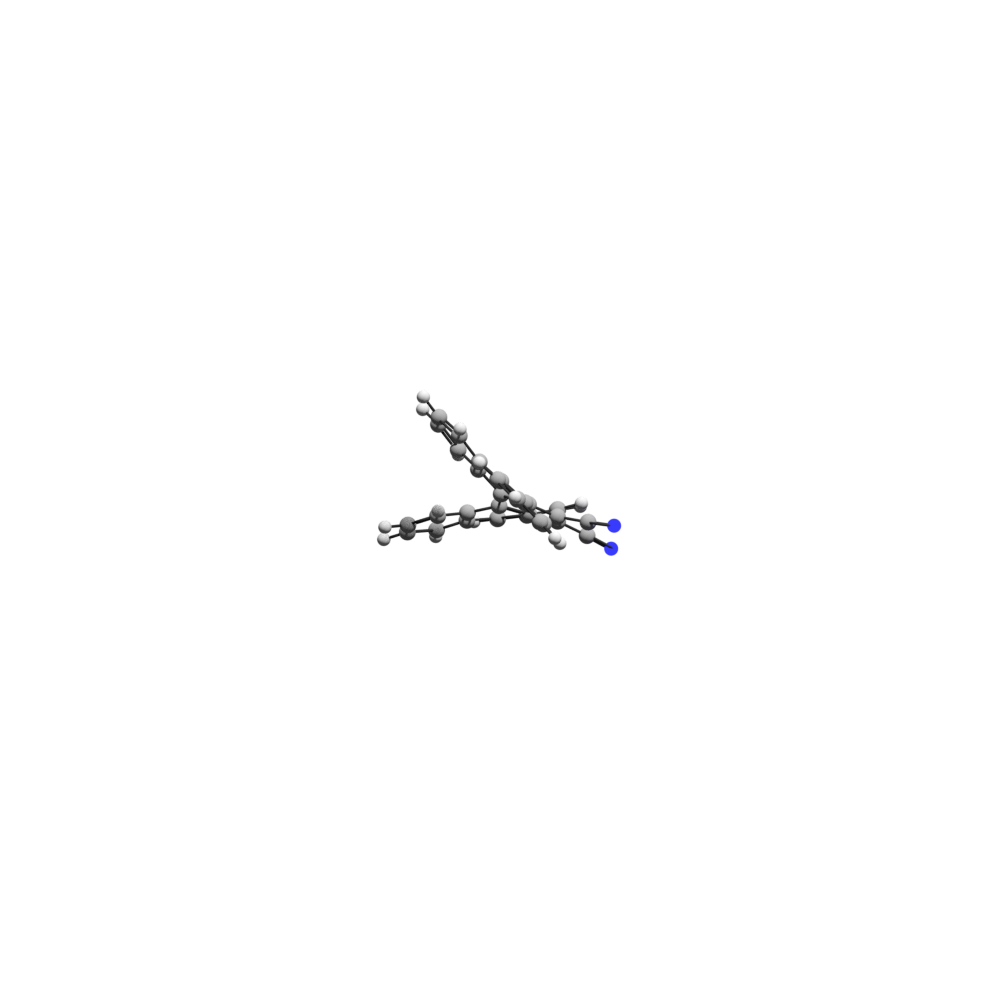
\includegraphics[width=0.3\textwidth]{./images/molecules/helicene-side}
			\label{fig:helicene-side}
		} \quad
		\caption{DCDB. \subref{fig:helicene-top} Top view, \subref{fig:helicene-side} side view}
		\label{fig:helicene}
	\end{figure}
	
	Helicenes were first synthezised in the 1950's \cite{Newman_synthesis_1956}. They consist of ortho condensed carbon rings that form a spiral due to overcrowding in their center. While they first drew attention due to their fluorescence properties \cite{vander_donckt_fluorescence_1968}, helicenes are interesting molecules because of their chiral feature. Two different turn directions exist, left and right.  
	
	In this work we investigate sub-monolayer coverages of 7,8-dicyano-5,6,9,10-dibenzo-[5]Helicene (dcdb-[5]H). The benzol groups condensed at positions 5,6,9,10 to the five carbon rings of [5]H (db-[5]H) are used to achieve a more distinct footprint of the molecule. Two cyano groups added at the central carbon ring induce a permanent dipole moment of 6.3 D (\autoref{fig:hel-fig1}a,b) and complete the molecule we use here. 

	For more information, please refer to \autoref{section:helicene}.
%\printbibliography
%%%%%%%%%%%%%%%%%%%%%%%%%%%%%%%%%%%%%%%%%%%%%
\chapter{Epitaxial hexagonal boron nitride on copper foils}
  \begin{itemize}	
	\item Challenges in mass production (example)
  	  \subitem Ease of use
 	  \subitem Costs
	    \subsubitem How to overcome (example)
\end{itemize}	

For this reason, we focused on the use of cheap substrates to achieve the very same functionality as on expensive single crystals. In this chapter copper foils are first chemically polished and prepared for investigation in AFM (p. \pageref{sec:foil-AFM}), SEM (p. \pageref{sec:foil-SEM}) and STM (p. \pageref{sec:foil-STM}). After CVD growth of \textit{h}-BN with borazine, foils are investigated in XPS (compare \autoref{fig:xps-self-grown}). A comparison to bought \textit{h}-BN foils is found at the end of the chapter.

Comparable experiments  are performed by \cite[8]{stables_report_2008}). 

\section{Pre-treatment of Cu-foils}
  \subsection{Electropolishing copper foils}
  As was mentioned before, clean, highly ordered surfaces are desirable to perform experiments on. Effort is done to clean the surfaces before every experiment to ensure a reproducible environment and interpretable results. This lead to a detailed understanding of the physics and chemistry behind a lot of systems. In case a systems order and functionality does not heavily depend on the substrates symmetry, single crystals loose most of their unique selling point. Instead of choosing a expensive bulk single crystal, thin copper foils can catch up in production environments. The mass produced foils still show some inconvenient properties. Although pure copper foils ($\geq \SI{99.999}{\percent}$) are available, their surface was never meant to be atomically flat. 
A representation of a copper surface before electro polishing can be seen in figure \ref{fig:copper-foil-grains}. Here the layered structure of the (mechanically polished) foil is apparent and shows different sizes of grains and annealing twins at the surface. Small subgrains constitute the uppermost layers, while deeper lying layers consist of larger grains with grain boundaries becoming more and more diffuse with increasing distance to the surface.

%\begin{figure}[]\centering
%	
%	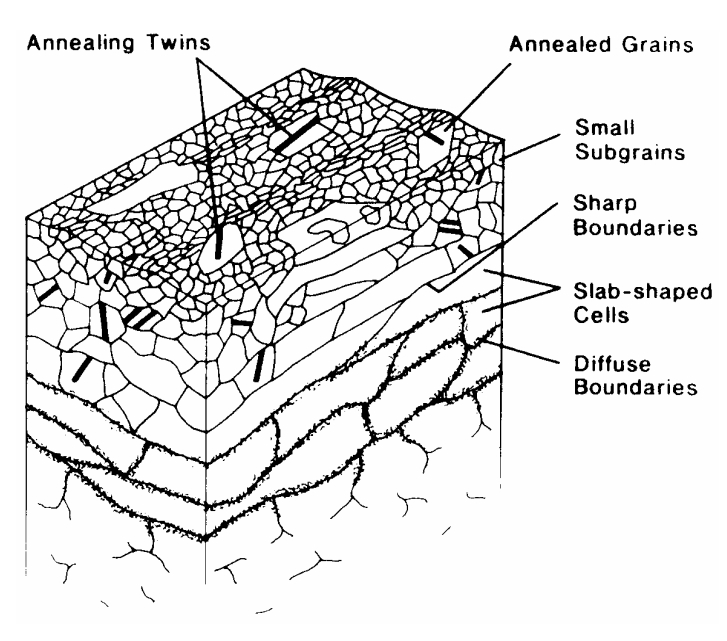
\includegraphics[width=0.45\textwidth]{./images/grain-structure-copper-foil}	
%	\caption{\ref{turley_nature_19810}}
%	\label{fig:}
%\end{figure}


\begin{wrapfigure}{r}{5cm}
	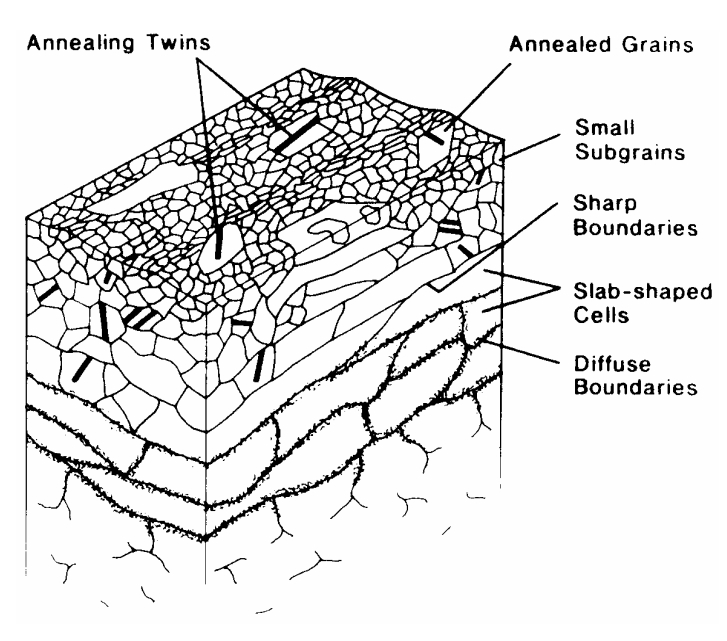
\includegraphics[height=40mm]{./images/grain-structure-copper-foil}
	\caption{Proposed bulk structure of a OFHC copper foil after abrasion with P1200 silicon carbide paper. Adopted from \cite{turley_nature_19810}}
	\label{fig:copper-foil-grains}
\end{wrapfigure}

But growing high quality ad-layers on polycrystalline copper foils requires a smooth surface. As-ordered Cu foils exhibit a root-mean-square (RMS) surface roughness of about \SI{218}{\nm}\cite{bin_zhang_low-temperature_2012}. Striations - a fabrication remnant due to the cold rolled foils - are observed on the surface\cite{kim_synthesis_2012-1}. Also some manufacturers apply a thin layer of chromium oxide for corrosion protection\cite{bin_zhang_low-temperature_2012}. A common procedure to reduce the roughness of a material is to electrochemical polish the surface.

A comprehensive overview of \index{electrochemical polishing} electrochemical polishing of Cu surfaces with different etchants can be found in \cite{jinshan_electrochemical_2004}. The following gives a short introduction in chemical polishing as used for preparation of thin copper foils.\footnote{For a broader view on the topic, the reader is pointed to references \cite{antoine_polishing_1999, lilje_improved_2004, schulz_engeneering_2018}.}

\paragraph{solution of anode atoms in aqueous cell medium}
Electrons and atoms at the solid surface have higher energy states. Thus some of the atoms on the metal surface may lose electrons to form ions. These ions may also recombine with electrons and become atoms at another moment. Depending on the electronic structures, some metals (such as sodium) are easier than others (such as platinum) to ionize. Copper is relatively stable. Still, some of the surface atoms may be expected to ionize at a moment. The ionization process may be promoted when the metal is in touch with aqueous solution because: 
\begin{itemize}
	\item Metal ions can not move in the metal electrode but can move through the solution, producing electric current in solution with an applied potential
	\item Electrons can move freely in metal solid (electric current in a metal) but can not survive in solution and will quickly recombine with positive ions
	\item Water dipoles and negative ions in solution may drag the surface metal ions into the solution
\end{itemize}

\paragraph{chemical reaction}\index{electrochemical polishing!chemical reaction}
``The electrode connected to the positive pole of the power supply is called anode. And the one connected to the negative pole of the power supply is called cathode. When the applied voltage is high enough, electrons in the anode may be pumped out and the metal atoms on the anode surface will be oxidized (e.g., $Cu - 2e = Cut^{2+}$) and dissolved into the electrolyte solution. Under electrical field, the positive ions (cations) move towards cathode and negative ions (anions) move towards anode. The cations may get electrons and be reduced to neutral atoms (e.g., $Cu^{2-} + 2e = Cu$) again at the cathode surface. Therefore, charge transfer between the two electrodes is carried out via the ion drift in the electrolyte and electron conduction in metal wire. When the working electrode is set to be anode, dissolution is processed at certain potential. Likewise, when the working electrode is set to be cathode, it can result in deposition. For electropolishing of copper, the copper part to be polished is set to be anode while the cathode can be any conductive material (e.g., copper).

The critical potential at which the oxidation / reduction starts to occur is related to the standard redox potential for a specific anode material. The redox potential $E_O$ is a measure (in volts) of the affinity of a substance for electrons - its electronegativity - compared with hydrogen (which is set at 0). Substances more strongly electronegative (i.e., capable of oxidizing or accepting electrons) than hydrogen have positive redox potentials (e.g., $Cu/CU^{2+}$: $E_O = \SI{0.34}{\volt}$). Substances less electronegative (i.e., capable of reducing or giving up electrons) than hydrogen have negative redox potentials (e.g., $Cr^{3+}/Cr^{2+}$: $E_O = \SI{-1.07}{\volt}$)\cite{jinshan_electrochemical_2004}

\paragraph{Removed mass from working electrode}
``The current flow of every two electrons results in one copper atom dissolved on the anode and deposited on the cathode. Since $\SI{1}{\ampere}= \SI{1}{\coulomb \second}$, the charge of one electron $e = \SI{1.60218E16}{\coulomb}$, so the number of electrons (per second) in 1 A current is $N_e = \frac{I}{e}$; the number of copper atoms being oxidized or reduced $N_a= \frac{1}{2} N_e= \frac{I}{2e}$, the number of moles $N_m = \frac{N_a}{N_A} = \frac{I}{2eN_A}= \frac{I}{2F}$ where Avogadro's number $N_A = \SI{6.02214E23}{\per \mole}$. The weight of $N_m$ mole copper $W = N_m M = \frac{IM}{2 F}$ where M is the molecular weight of copper. Thats a volume, $V = W / d =\frac{IM}{2 F d}$ where d is the density of copper. Thus a current I produces a dissolution/deposition rate in thickness (\SI{}{\centi\meter \per \second}) \begin{equation} R_d=\frac{M}{2 FdA}I \label{dissolution-rate}\end{equation}
where A is the area of the electrode surface.
\cite[34]{jinshan_electrochemical_2004}

\paragraph{Voltage-current-characteristic or polarization curve}
\begin{itemize}
	\item[-]On a polycrystalline metal surface there are sites, such as defects and grain boundaries, where atoms are at higher energy states. In addition, due to arbitrary crystal orientation, there are different crystalline planes with different energy states of atoms on the electrode surface. Therefore, atoms at all these different sites and planes have different standard redox potential $E_O$, and as a result, have different dissolution rate according to eq. \ref{dissolution-rate}. Such an anodic dissolution will not lead to polishing. Instead, a crystallographic etching is produced (reference [9, 33-35] within \cite{jinshan_electrochemical_2004}). This is true at lower current (or applied potential). This refers to the \textbf{"etching"} regime in figure \ref{fig:oxygen-pitting} with $U<\SI{1.5}{\volt}$.
	\item[-]The plateau where the current remains almost constant with increasing voltage is referred to as \textbf{"polishing plateau"}. Overall, the values of iL and EL of the limiting current plateau and the shape of a polarization curve depends on electrolyte solution, anode material, disk rotating speed, solution circulation, temperature, and the distance between anode and cathode.
	Of all the factors, electrolyte is the most important one determining the polarization curve.
	\item[-]With continuing increase of applied potential, other reactions than Cu oxidation and reduction may occur and contribute to the increasing current. These reactions produce $H_2$ and $O_2$ bubbles, which occur at or reach the anode surface. This is known as \textbf{"oxygen pitting"}.
\end{itemize}

\paragraph{gas bubbling}
Gas (oxygen or hydrogen) bubbles may block $Cu^{2+}$ ion transport and therefore terminate the electrochemical dissolution process on the area inside the bubbles. However, the residual solution on the surface area inside the bubbles may react with Cu atom and result in chemical etching. Depending on the chemical property of the electrolyte solution and the value of current density at which the electrochemical dissolution is occurring, the etching speed can be higher than the rate of electrochemical dissolution. In this case, pits will be produced on the anode and produce a rough surface. If etching does not occur inside the bubbles, or if its speed is slower than that of electrochemical dissolution process, the area inside the bubbles will remain and appears as protruding particles after the electrochemical dissolution process. In either case, a rough surface is produced. Approaches to reduce the effect of oxygen bubbling are done by altering the etching solution with different additives.

\begin{figure}\centering
	\subfigure[Sketch of a typical setup used for electro polishing. A beaker is used to hold the aqueous cell medium. The copper foil and a counter electrode are immersed and connected a the + and - connections of a DC power supply. Image reproduced from \cite{stables_report_2008}]{
		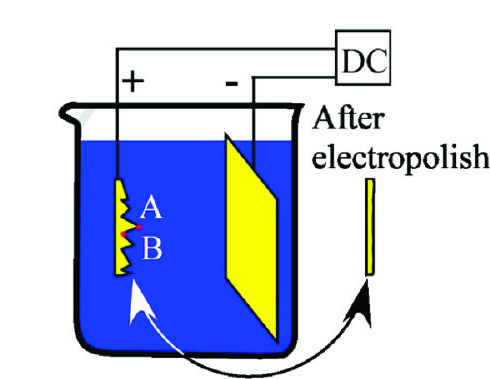
\includegraphics[width=0.4\textwidth]{./images/cm1028854-fig2-d}
		\label{fig:etching-setup}
	} \qquad%
	\subfigure[Current-voltage characteristic indicating different phases in the ething and polishing process. While at low voltage etching is the dominant process, a polishing plateau is formed at intermediate voltages. Exceeding a threshold leads to increased formation of excess oxygen in the oxygen pitting regime. \cite{luo_effect_2011}]{
		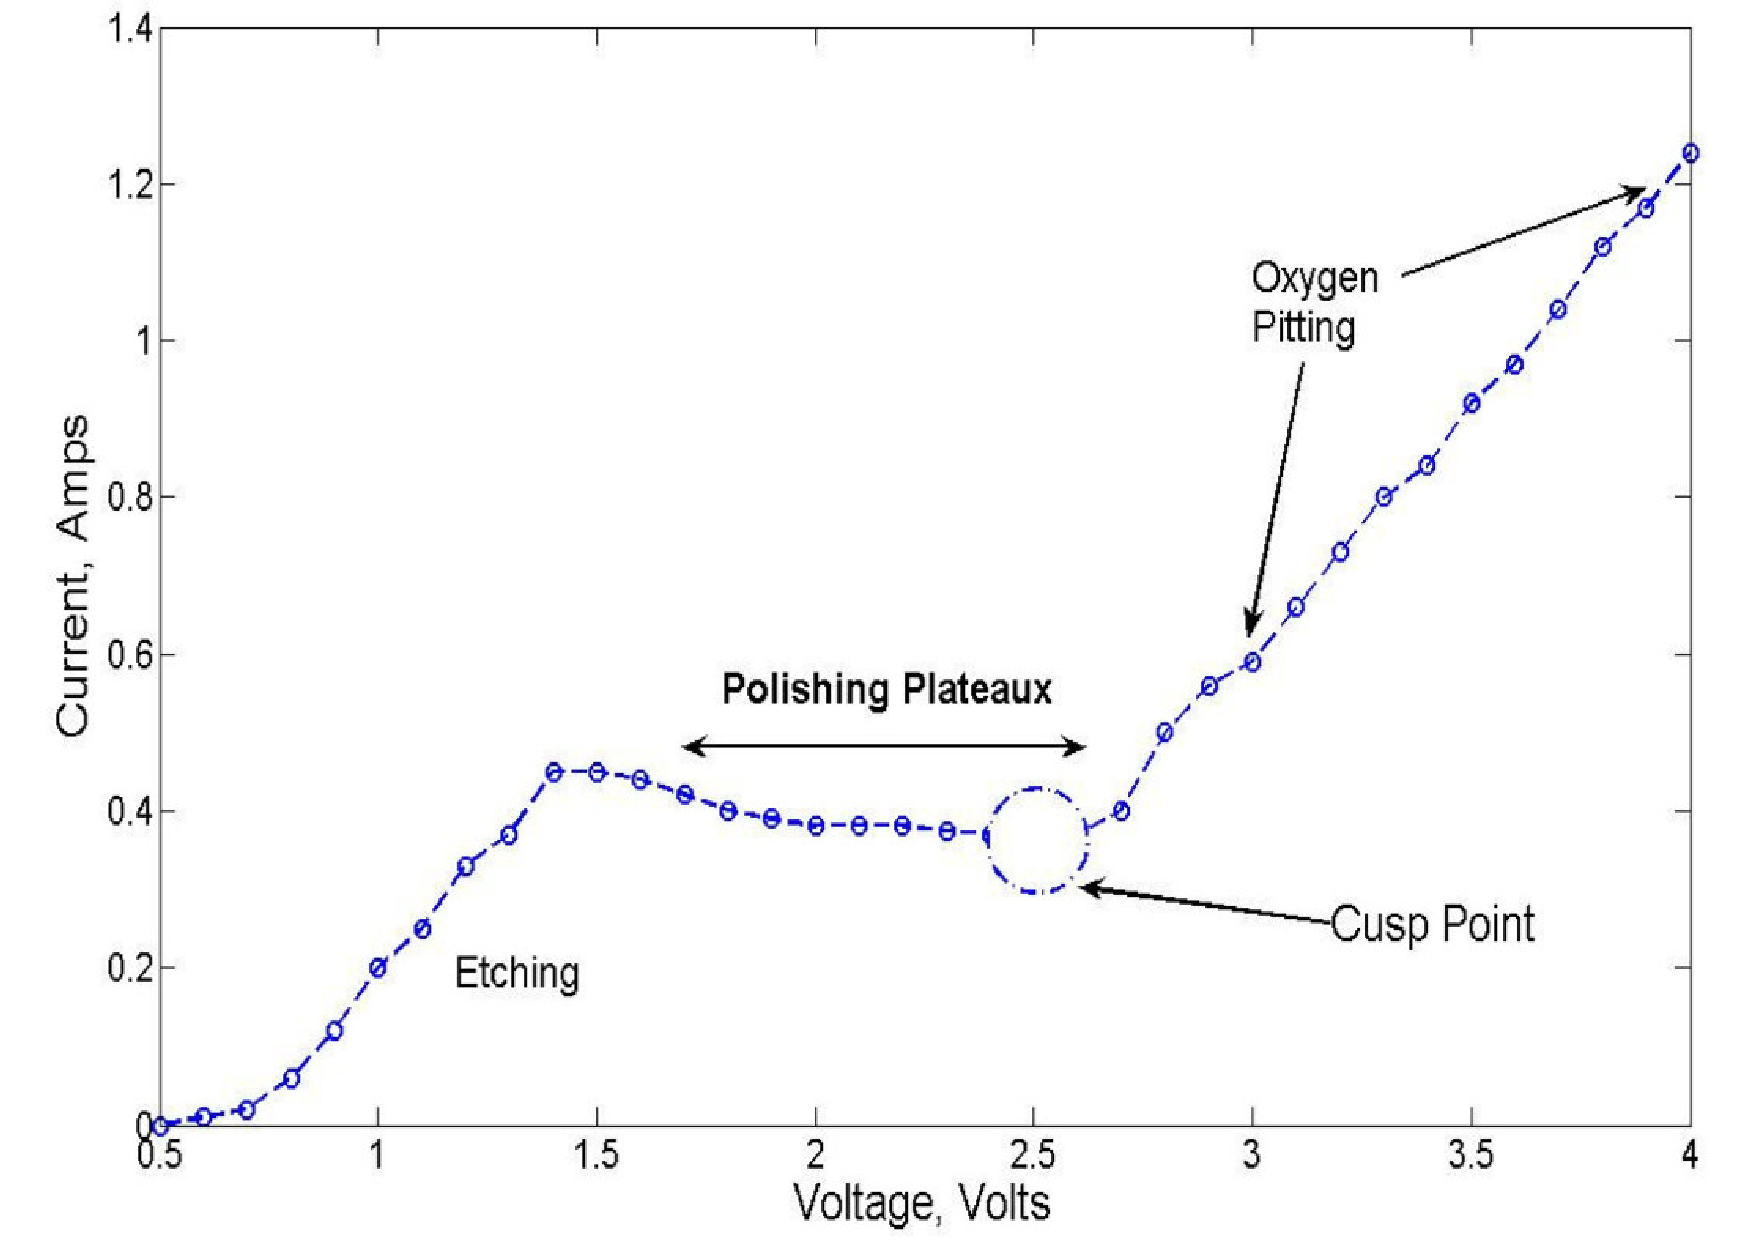
\includegraphics[width=0.4\textwidth]{./images/oxygen-pitting}
		\label{fig:oxygen-pitting}
	}
	\caption{Experimental setup and voltage characteristic used for electrochemical polishing. \ref{fig:etching-setup} In the process the foil is connected as working electrode (+) and opposed by a counter electrode (-). Material is then transported from the working to the counter electrode resulting in a polished foil surface. \ref{fig:oxygen-pitting} Choosing proper voltage and current values in the polishing plateau is important for good results.}
	\label{fig:setup-and-characteristic}
\end{figure}

%%%%%%%%%%%%%%%%%%%%%%%%%%%%%%%%%%%%%%%%%%%%%%%%%%%%%%%%%%%%%%%
%%% ################## minipage for table ##################
%\begin{table}[!h]
%	\centering
%	\caption{Used chemicals for the etching process}
%	\begin{tabular}{lll}
%		Linear formular & Common name & Fully systematic additive name \\ \hline \hline
%		$CH_3CH_2OH$   & Ethanol &  Ethanol \\
%		$H_3PO_4$ & (ortho-)Phosphoric acid & Trihydroxidooxidophosphorus  \\
%		$NH_2CONH_2$ & Urea & Carbonyldiamide \\
%		$(CH_3)_2CHOH$  & Isopropanol &  2-Propanol \\
%		$CH_C(OH)[PO(OH)_2]_2$& HEDP, Etidronic acid &  1-Hydroxyethane-1,1,-diphosphonic acid \\
%		$[H(OCH_2CH_2)]_nOH$ & (P)EG & (Poly-)Ethylene Glycol\\
%		%$H_2PO_4^{-1}$ & Dihydrogenphosphate & Dihydroxidooxidophosphorus(1-)  \\
%		%$HPO_4^{-2}$ & Hydrogenphosphate & Hydroxidooxidophosphorus(2-)  \\
%		%$[PO_4]^{-3}$ & Phosphate & Tetraoxidophorsphate(3-)  \\ \hline
%	\end{tabular}
%	\label{tab:small-molecules}
%\end{table}
%%%% ################## minipage for table ##################
%\begin{figure}[!h]
%	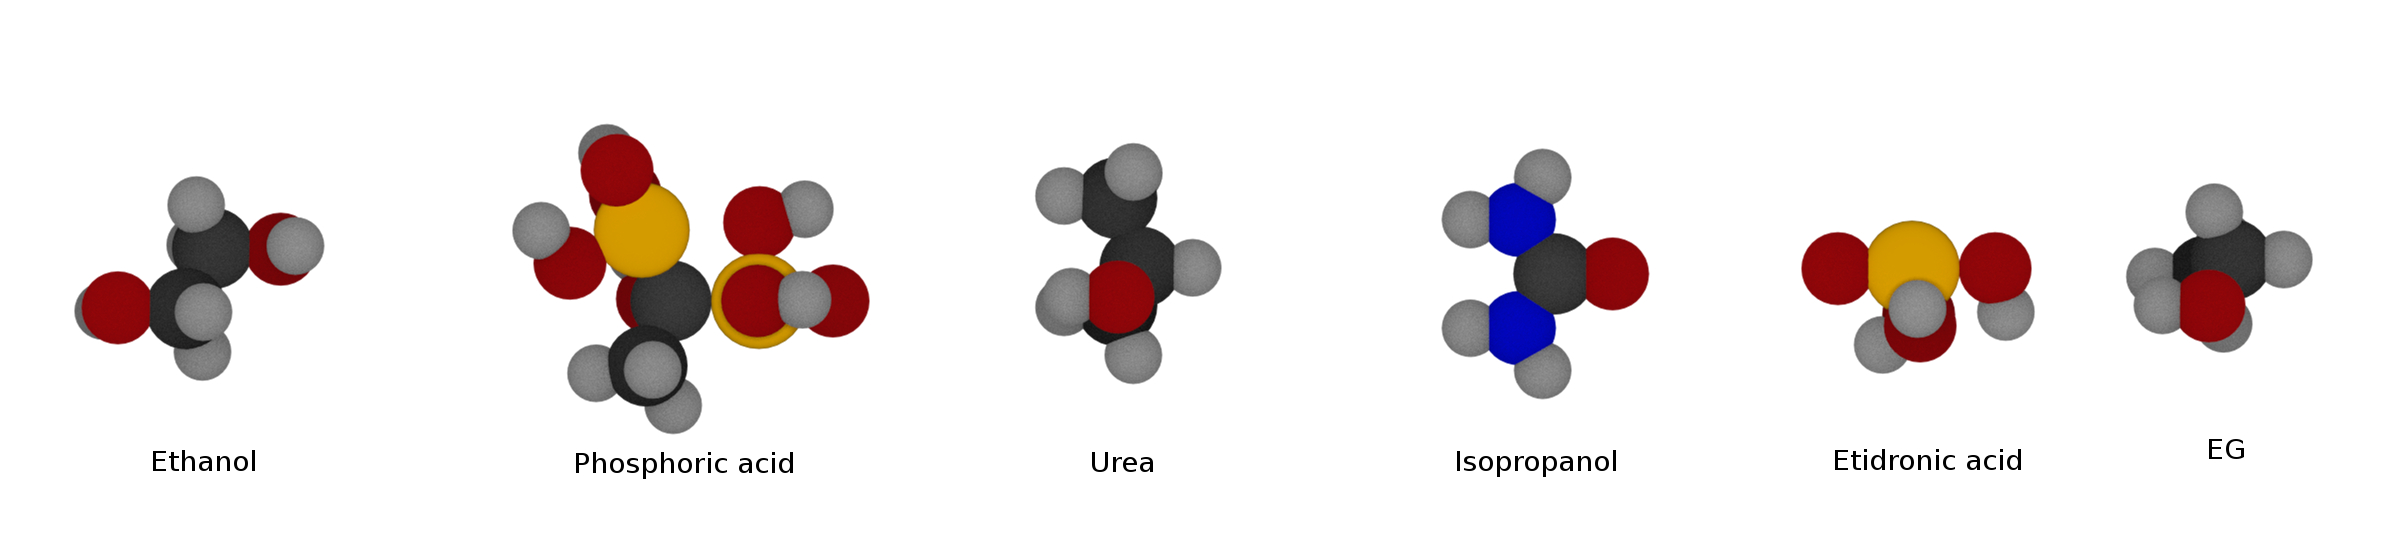
\includegraphics[angle=0,width=\textwidth]{./images/small-molecules-leabelled.jpg}
%	\caption{Molecules from table \ref{tab:small-molecules}, in order from top to bottom (left to right).}
%\end{figure}

%%%%%%%%%%%%%%%%%%%%%%%% molecules in structure formulas %%%%%%%%%%%%%%%%%%%%%%%% 
% \begin{figure}[h!]
% \centering
% \subfigure[Structure of HEDP(CAS number is 2809-21-4\cite{_hedp_2014}). Image taken from \cite{_hedp_wiki_2014}]{
% 	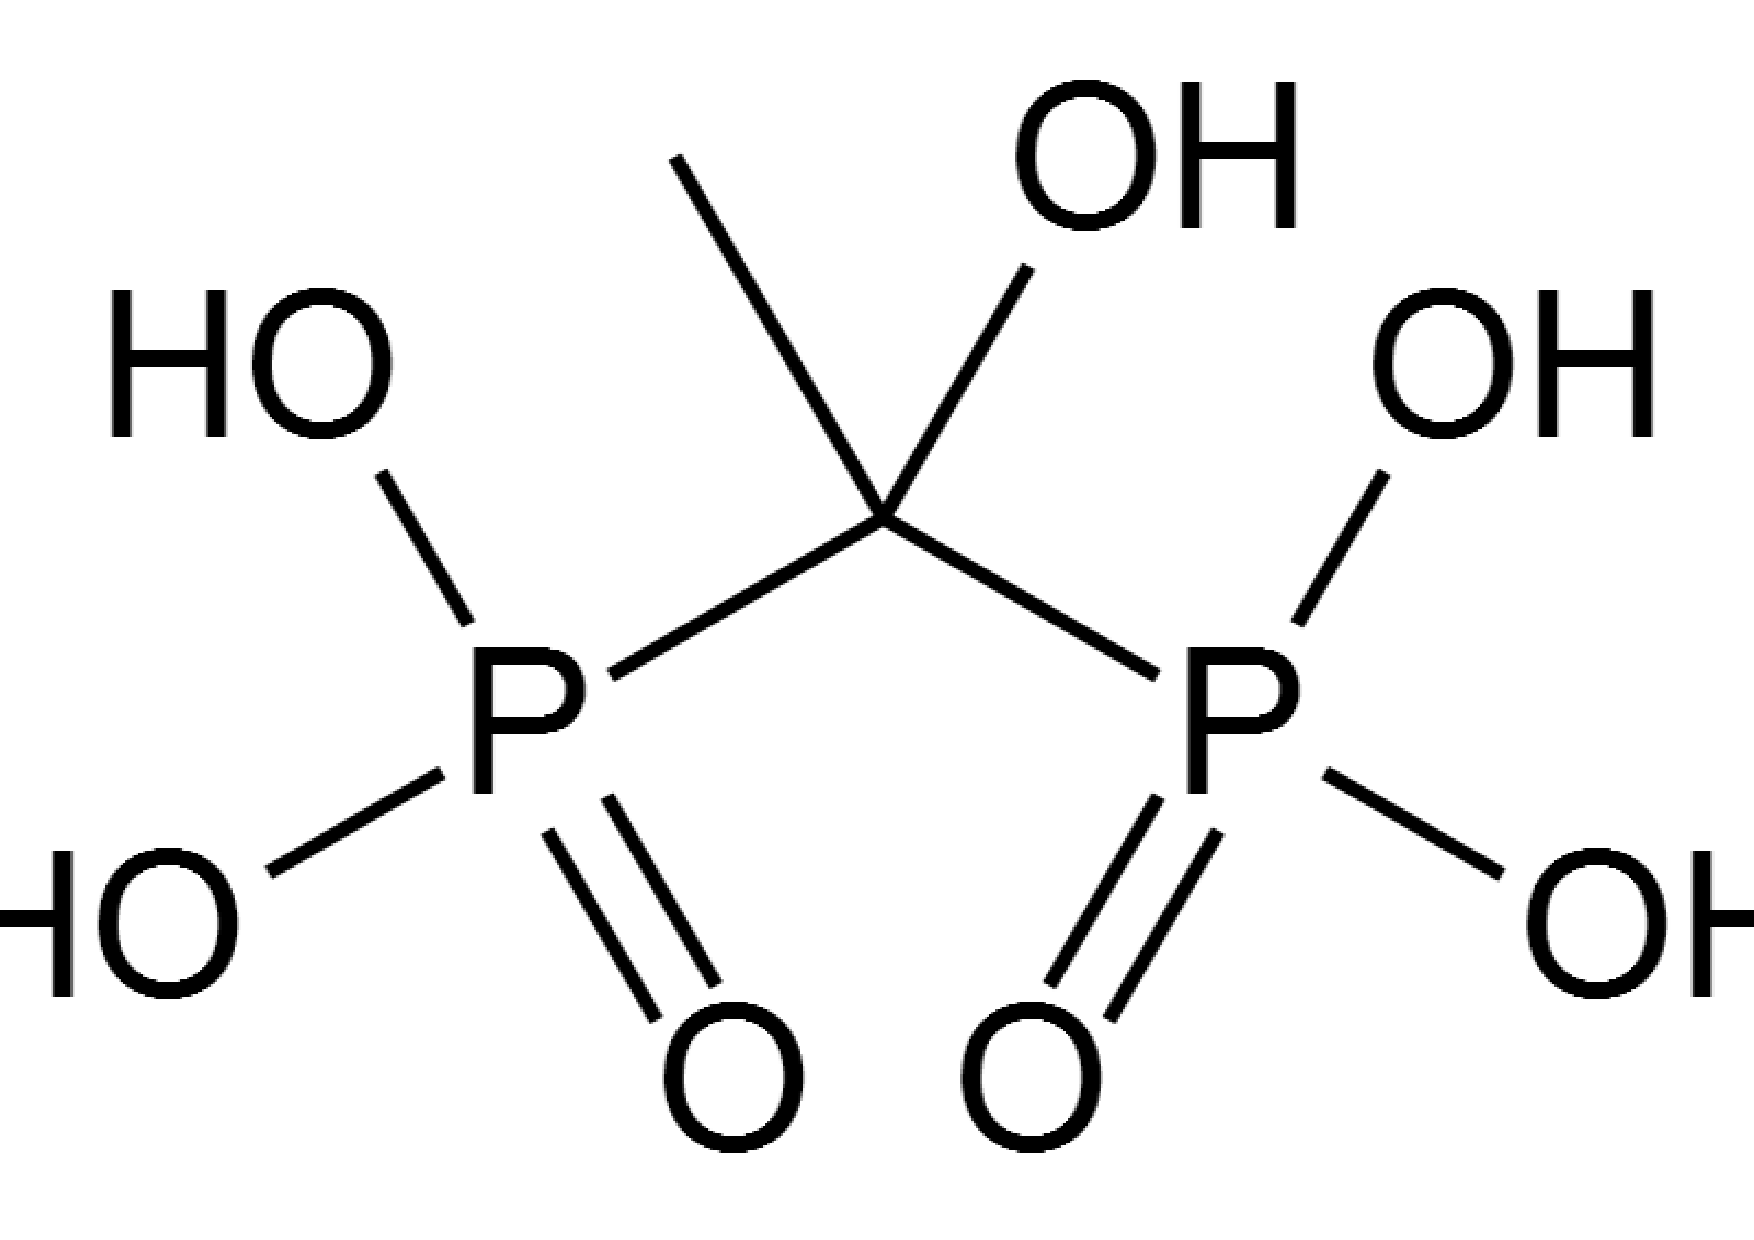
\includegraphics[width=0.45\textwidth]{./images/Etidronic_acid}
% }
% \subfigure[Structure of phosphoric acid(CAS number is 7664-38-2). Modified from \cite{_phosphoric-acid-2d-dimensions.png_2014}]{
% 	
\includegraphics[width=0.45\textwidth]{./images/Phosphoric-acid-2D-dimensions}
% }
% \caption{Different phosphoric acids}
% \end{figure}
% 
% \begin{figure}[h!]
% \centering
% \subfigure[Structure of 2-Propanol (CAS number 67-63-0). Image taken from \cite{_isopropyl_2014}]{
% 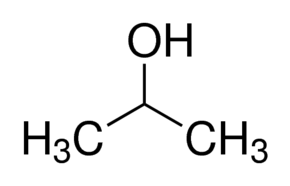
\includegraphics[width=0.45\textwidth]{./images/2-Propanol}
% 	}
% \subfigure[Structure of Ethanol (CAS number 64-17-5). Image taken from \cite{_64-17-5_2014}]{
% 	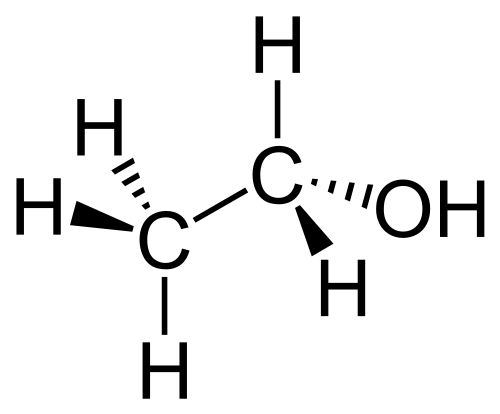
\includegraphics[width=0.45\textwidth]{./images/Ethanol}
% 	}
% \caption{Different alcohols}
% \end{figure}
% 
% \begin{figure}
% \centering
%   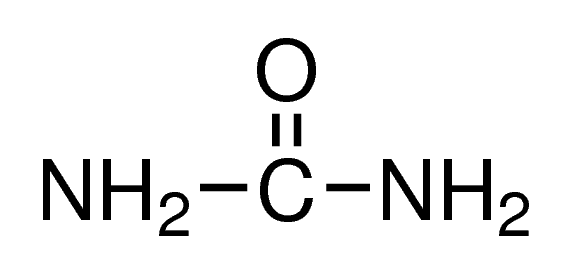
\includegraphics[width=4cm]{./images/urea}
% \caption{Structure of urea(CAS number is 57-16-6). Image taken from \cite{_urea_2014}}
% \end{figure}
% 
% \begin{figure}
% \centering
%   \includegraphics[width=4cm]{./images/poly(ethylene-glycol)}
% \caption{Structure of PEG (CAS number 25322-68-3). Image taken from \cite{_polyethylene_2014}}
% \end{figure}
%%%%%%%%%%%%%%%%%%%%%%%% molecules in structure formulas %%%%%%%%%%%%%%%%%%%%%%%% 
\paragraph{Etching solutions in literature} 
To find the most adequate polishing recipe, the most common ones have been reviewed and will be shown in the following. Many etching processes of Cu foils base of phosphoric acid that is refered to as ortho-phosphoric-acid, too. Liquid phosphoric acid is an 85\% aqueous solution. \cite{_7664-38-2_2014} 

%%%%%%%%%%%%%%%%%%%%%%%%%%%%%%%%%%%%%%%%%%%%%%%%%%%%%%%%%%%%%%%%%%%%%%%%%%%%%%%%%%%%%%%%%%%%%%%%%%%
Here (table \ref{tab:etching-recipes}), some of the etching recipes are given as reported in literature. They all have been used to electrochemically polish the Cu foil prior to graphene or boron nitride growth. We will discuss the used recipes in the following with focus on the additives used.

\begin{table}[] \centering
	\caption{Table with some of the found etching recipes.}
	\begin{tabular}{lcccc}
		& unit 			& \cite{luo_effect_2011} & \cite{stables_report_2008} & \cite{bin_zhang_low-temperature_2012} \\ \hline 
		$H3PO_4$	&[\SI{}{\milli\liter}]  & 300   & 100	& 50 \\
		$H_2O$		&[\SI{}{\milli\liter}]	& ---	& ---	& 100 \\
		2-Propanol	&[\SI{}{\milli\liter}]	& ---	& ---	&  10 \\
		Ethanol		&[\SI{}{\milli\liter}]	& ---	& ---	&  50 \\
		Butanol		&[\SI{}{\milli\liter}]	& ---	& ---	& --- \\
		Urea		&[\SI{}{\gram}]		    & ---   & ---	& 1 \\
		(P)EG		&[\SI{}{\milli\liter}] 	& 100	& 0.1  	& --- \\
	\end{tabular}
	\label{tab:etching-recipes}
\end{table}
%%%%%%%%%%%%%%%%%%%%%%%%%%%%%%%%%%%%%%%%%%%%%%%%%%%%%%%%%%%%%%%%%%%%%%%%%%%%%%%%%%%%%%%%%%%%%%%%%%%
Different additives to the acid are used to gain a better control of the etching process.  A typical one is PEG.\footnote{Further additives are used in etching solutions. Isopropanol and Ethanol are introduced for a more stable current density. HEDP increases the critical current density in phosphoric acid solutions\cite{jinshan_electrochemical_2004} and therefore the reaction rate. Citric acid is also used at low concentrations \SI{1000}{pppm} \cite{chang_superpolishing_2003}}  

One may add PEG for reduced oxygen bubbling during the process (compare fig. \ref{fig:oxygen-pitting})\cite{stables_report_2008,chang_superpolishing_2003}. It was shown that a concentration of \SI{1000}{ppm} PEG decreases the amount of oxygen pits. A comparison between electro polished foils with and without PEG are shown in figure \ref{PEG-additive}. After etching with purely phosphoric acid the surface remains rough and covered with pits. After adding PEG to the polishing solution the resulting foil shows a smoothened surface with little oxygen pits left.

\begin{figure}\centering
	\subfigure[Surface characterization with an interferometer. Oxygen pits are clearly visible in (A) while after adding \SI{1000}{ppm} PEG to the polishing solution greatly reduced their amount and smoothes the surface (B). See \cite{stables_report_2008}]{
		\includegraphics[width=0.9\textwidth]{./images/copper-foil-oxygen-pits.jpg}
		\label{fig:PEG-additive-1}
	} \qquad%
	\subfigure[(a-b) Copper foil before and after etching with \SIrange{1}{2}{\volt} for \SI{0.5}{\hour} following recipe \cite{luo_effect_2011}. Corresponding height profiles are shown in (c). Adopted from \cite{luo_effect_2011}]{
		\includegraphics[width=0.9\textwidth]{./images/cm1028854-fig2-a-c.jpg}
		\label{fig:PEG-additive-2}
	}
	\caption{Effect of adding PEG to the etching soltution. Interferometric and AFM topography images before and after polishing.}
	\label{fig:PEG-additive}
\end{figure}

%\paragraph{Notes to etching recipes}
%\begin{itemize}
%
%	\item[\cite{stables_report_2008}] Mechanically polished with silicon carbide paper (wet-dry / \SIrange{1200}{6000}{} prior to etching)
%	\item[\cite{luo_effect_2011}]
%	\begin{itemize}
%		\item rough polished with fine metal paste, cleaning in ethanol with sonication 
%		\item soldlered to metal wire, covered with silicone gel on back, edges and corners
%		\item etching in solution, foil used as work- (+) and copper plate as counter-electrode (-) 
%		\item \SIrange{1}{2}{\volt} for \SI{0.5}{\hour} 
%		\item wash with deionized water with sonication, neutralize acid remnants with amonia solution (\SI{1}{\percent})
%		\item wash with ethanol and blow dry with nitrogen, remove silicone gel and store in ethanol
%	\end{itemize}
%\end{itemize}
%%%%%%%%%%%%%%%%%%%%%%%%%%%%%%%%%%%%%%%%%%%%%%%%%%%%%%%%%%%%%%%%%%%%%%%%%%%%%%%%%%%%%%%%%%%%%%%%%%%
A detailed investigation on polishing solutions based on phosphoric acid can be found in \cite{jinshan_electrochemical_2004}. It was found that adding EG into phosphoric acid solutions decreases the  limiting current. The more EG added the lower the limiting current. This is true for both undiluted and diluted (with deionized water) phosphoric acid solution. Diluting phosphoric acid - EG solutions with water (25\%, curve 2 in Fig. 3-10 within \cite{jinshan_electrochemical_2004} ) increases limiting current as shown in table \ref{table:used-etching-solutions}. Further diluting phosphoric acid - EG solutions with water (5O\%, curve 3 in Fig. 3-10 (within \cite{jinshan_electrochemical_2004} )) decreases limiting current. Limiting current plateau disappears at \SI{12.5}{\percent} phosphoric acid + \SI{37.5}{\percent}EG + \SI{50}{\percent} water. 
%%%%%%%%%%%%%%%%%%%%%%%%%%%%%%%%%%%%%%%%%%%%%%%%%%%%%%%%%%%%%%%%%%%%%%%%%%%%%%%%%%%%%%%%%%%%%%%%%%%
As the etching times are quiet long, efforts have been made to reduce the polishing time by varying the polishing solution. Results with a more complicated etching recipe \cite{bin_zhang_low-temperature_2012} are depicted in figure \ref{fig:etching-bin-zhang}. Here the etching was performed with a large copper plate used as cathode. Alligator clamps are used to apply a voltage of \SIrange{3}{6}{\volt} between the foil and the plate. The foil is used as anode (+). After \SI{1}{\minute} the foil is taken out and rinsed with deionized water, further washed with ethanol, and then dried with compressed nitrogen gas. 

The height profile of the copper foil surface before and after treatment indicate diminishing striation height and overall roughness from $\approx \SIrange{218}{64}{\nano \meter}$ within a very short period of time. Although the surface is still rather irregular, a dominant orientation of the remaining grains is observed in the (001) direction and helps the subsequent growth of graphene with toluene to form rectangular flakes.

%\begin{figure}[h]
%	\begin{center}
%
%	\end{center}
%	\caption{Height profiles before (a) and after (b) \SI{1}{\minute} electro polishing with a solution reported in \cite{bin_zhang_low-temperature_2012}. The linear striations, caused by mechanical processing of the copper foil, and the overall roughness of the surface decrease.}
%	\label{fig:etching-bin-zhang}
%\end{figure}

\begin{figure}\centering
	\subfigure[Noncontact optical profilometer scans in VSI mode of unpolished (top) and polished (bottom) Cu-foil surface.]{
		\includegraphics[height=0.6\textwidth]{./images/0fcfd512d196815269000000-fig1.jpg}
		\label{fig:fig:etching-bin-zhang-profile}
	}\qquad 
	\subfigure[SEM images after graphene growth with a toluene precursor at \SI{550}{\celsius}]{
		\includegraphics[height=0.6\textwidth]{./images/copper-foil-graphene-growth.jpg}
		\label{fig:fig:etching-bin-zhang-growth}
	}
	\caption{Height profiles and SEM images before and after \SI{1}{\minute} electro polishing with a solution reported in \cite{bin_zhang_low-temperature_2012}. The linear striations, caused by mechanical processing of the copper foil, and the overall roughness of the surface decrease after polishing. Graphene coverage is increased under the same growth conditions, solely through better substrate conditions.}
	\label{fig:}
\end{figure}

%%%%%%%%%%%%%%%%%%%%%%%%%%%%%%%%%%%%%%%%%%%%%%%%%%%%%%%%%%%%%%%%%%%%%%%%%%%%%%%%%%%%%%%%%%%%%%%%%%%
%To further improve the surface properties of the polished copper foil, other recipes have been developed
%  \item 
% \begin{table}[h!]
% \centering
%   \begin{tabular}{lll} 
%   HEDP & \SI{30}{\percent} & \SI{60}{\ml} \\
%   $H_3PO_4$ & \SI{30}{\percent} & \SI{60}{\ml}\\
%   $H_2O$ & \SI{40}{\percent} & \SI{80}{\ml}\\
%   PEG & \SI{1000}{ppm} & \SI{0,2}{\ml}\\
%  \end{tabular}
% \caption{Etching recipe knowkn source}
% \end{table}

%  Removal rates are about \SI{1.8}{\mu \meter \per \min}


\paragraph{Experimental setup}

\paragraph{Used solution}\index{electrochemical polishing!Used solutions}
Within this work, Cu-foil polishing will be done with recipe I broken down in table \ref{tab:used-etching-solution}. It has several advantages. Since the main goal is the achieve a virtually flat surface, the resulting roughness of the surface is the most important parameter. In contrast to etching recipes without PEG (where oxygen pitting is an issue) and more complex etching recipes (to reduce etching time on exchange on surface roughness) a simple etching solution is chosen.

\begin{table}\centering
	\caption{Used etching solutions (compare \cite[130]{jinshan_electrochemical_2004}). Note the change in the removal rate due to higher limiting currents in the solution after adding ethylene-glycol to the solution.}
	\begin{tabular}{lcc}
		& I & II \\ \hline \hline
		$\SI{85}{\percent} H_3PO_4$ & 70 & 100 \\
		Ethylene-gylcol & 5 & 0 \\
		Deionized water & 25 & 0 \\ \hline
		Potential [\SI{}{\V}] & \multicolumn{2}{c}{\SI{1.2}{}} \\
		Current [\SI{}{\mA}] & 46 & 12\\
		Roughness [\SI{}{\nm}] & \multicolumn{2}{c}{\SI{5}{}} \\
		Removal rate [\SI{}{\micro\meter\per\minute}] & \SI{1,0}{} & \SI{0,26}{}\\
	\end{tabular}
	\label{table:used-etching-solutions}
\end{table}

\begin{table}
	\centering
	\caption{Volume and mass fractions for copper foil etching solution.}
	\begin{tabular}{lcccc}
		&unit	&$H_3PO_4$ (85\%)&	EG	&	$H_2O$	\\
		Dichte $\rho$   &[$g/cm^3$]	&	1.87	&	1.11	&	1.00	\\
		$1/rho$		&[$cm^3/g$]	&	0.54	&	0.90	&	1.00	\\
		Anteil 		& \%		&	70	&	5	&	25	\\ \hline
		Menge gesamt    &[$cm^3$]	&		\multicolumn{3}{c}{150} 	\\
		Menge anteilig  &[$cm^3$]	&	105.00	&	7.50	&	37.50	\\
		Gewicht         &[g]		&	196.35	&	8.33	&	37.50	\\
	\end{tabular}
	\label{tab:used-etching-solution}
\end{table}

%\paragraph{experimental things in \cite{jinshan_electrochemical_2004}}
%\begin{itemize}
%	\item[-]The distance between working and counter electrodes was about 15 mm. All experiments were carried out in a 200 mL glass container at room temperature. 100 mL electrolyte solution was used for each experiment.
%	\item[-]Adding EG into phosphoric acid solutions decreases limiting current. The more EG added the lower the limiting current. This is true for both undiluted and diluted (with water) phosphoric acid solution. Dilyuting phosphoric acid - EG solutions with water (25\%, curve 2 in Fig. 3-10) increases limiting current. Further diluting phosphoric acid - EG solutions with water (5O\%, curve 3 in Fig. 3-10) decreases limiting current. Limiting current plateau disappears at solution "12.5\% phosphoric acid + 37.5\% EG + 50\% water.\cite{jinshan_electrochemical_2004}
%\end{itemize}

%
%The given roughness in table \ref{table:used-etching-solutions}is much lower compared to references (\SI{61}{\nm})\cite[2]{bin_zhang_low-temperature_2012} that did the polishing with another recipe (compare table \ref{tab:etching-recipes}). Although the roughness is higher, optical profiler images indicate removed striations and a smoother surface compared to the as-bought foils (\SI{218,56}{\nm})\cite[2]{bin_zhang_low-temperature_2012}.

\paragraph{The etching process}
The etching process relies on the fact that the current density (and thus the etching rate) is higher in protruding regions of the copper foil (Ohmic leveling).  As a result the surface of the copper foil will be smoothened \cite{luo_effect_2011}. Compare with migration smoothing and diffusion smoothing\cite{jinshan_electrochemical_2004}.
%   \subsection{STM of 0.25mm Cu-foils}
%      The bought and chemically polished foils are mounted on a sample holder and loaded into the load lock. It is evacuated for \SIrange{2}{3}{\hour} and the valve is opened to the chamber. During transfer, no noteable increase in the base pressure is noted. The sample is put on the parking slot.

The sample was initially degased with slowly increasing temperatures to remove adsorbats like $CO, CO_2$ and $H_2O$.

After some time of degassing, the sample was prepared with repeated sputter and anneal cycles. The annealing temperatures were increased up to \SI{800}{\degreeCelsius}. 
After that procedure, the sample was cooled down and observed in STM.

\begin{figure}[h!]
 \centering
 \includegraphics[width=0.5\textwidth]{./images/F150331-125720.jpg}
 \caption{Cu-foil after repeated sputtering and annealing cycles. The roughness is about \SI{72}{\pico\meter}}
 \label{fig:cu-foil-clean}
\end{figure}

A first look onto the sample shows a quite heterogen surface. While quite flat areas with a typical roughness of $\approx \SI{70}{\pico\meter}$ exist, there are also areas with very large corrugations $\geq \SI{100}{nm}$.
%   \subsection{AFM of 0.25mm Cu-foils}
%      \paragraph{AFM}
\begin{figure}[h]
 \centering
 \includegraphics[width=0.4\textwidth]{../Daten/AFM/2015-01-15/as_bought0000.jpg}
 \includegraphics[width=0.4\textwidth]{../Daten/AFM/2015-01-15/as_bought0001.jpg}
 \caption{\SI{0.25}{\mm} as bought from alfa aesar, RMS$\approx$\SI{13}{\nm}, contrast \SI{100}{\nm} ($\approx$ RMS \SI{5}{\nm}, contrast \SI{70}{\nm} in the smaller image)}
\end{figure}
One can see the striations that stem from the production process (from top to buttom).
\begin{figure}[h]
 \centering
 \includegraphics[width=0.4\textwidth]{../Daten/AFM/2015-01-15/polished0000.jpg}
 \includegraphics[width=0.4\textwidth]{../Daten/AFM/2015-01-15/polished0001.jpg}
 \caption{\SI{0.25}{\mm} polished 5h in in 75/20/5 phosphoric acid, RMS$\approx$\SI{9}{\nm} in the over all image, contrast \SI{100}{\nm} ($\approx$\SI{5}{\nm} in the smaller image, contrast \SI{70}{\nm})}
\end{figure}
After etching ($U=1.2V$,I=\SIrange{120}{250}{\mA}) \SI{5}{\hour} in a solution \SI{75}{\percent} \SI{20}{\percent} \SI{5}{\percent} (Phosphoric acid, purified water, EG) the striations have gone and the RMS value decreased by \SIrange{30}{45}{\percent} (protrusions due to dirt in the image are counted).
The circular hole is an effect of bubbles in the etching process where the bubble affects the rate of etching. The over all structure changes from a very fuzzy and heterogenous sample height to a flat height contribution with only a little amount of defects. Those are sufficiently seperated in space to exhibit flat regions where the h-BN may grow unperturbated.
\begin{table}
\centering
\caption{Volume and mass fractions for copper foil etching solution.}
\begin{tabular}{lccc}
			&$H_3PO_4$ (85\%)&	EG	&	$H_2O$	\\
Dichte [$g/cm^3$]	&	1.87	&	1.11	&	1.00	\\
$1/rho$			&	0.54	&	0.90	&	1.00	\\
Anteil \%		&	70	&	5	&	25\\
Menge gesamt [$cm^3$]	&		\multicolumn{3}{c}{150} \\
Menge anteilig [$cm^3$]	&	105.00	&	7.50	&	37.50	\\
Gewicht [g]		&	196.35	&	8.33	&	37.50	\\
\end{tabular}
\end{table}

Some foil has been mechanically polished with 4k paper and several hours of Syton polishing. The roughness of these samples has been investigated also in AFM. These are compareable to the chemically polished ones, but are always slightly higher by $\approx 10\%$. Sometimes unwanted new scratches appear after mechanical polish.
  \section{STM of BN on Cu-foil(0.25mm)}
     % Beamtime April 2015
Further experiments were carried out to increase the cleanliness of the \textit{h}-BN on the polycrystalline copper foil. To reduce the amount of elements coming from the body of the foil, it is repeatedly sputtered and annealed to temperatures as high as \SI{800}{\degreeCelsius}. This may have also an improving influence on the grain size and amount of corrugation. Several attempts have been made which are described in summary below.
%%%%%%%%%%%%%%%%%%%%%%%%%%%%%%%%%%%%%%%%%%%%%%%%%%%%%%%%%%%%%%%%%%%%%%%%%%%%%%%%%%%%%%%%%%
\begin{itemize}
 \item After cleaning, the sample is investigated in STM. The foil shows a inhomogeneous topography, with parts of the sample showing very flat regions (figure \ref{fig:30-31.03}) while others still remain heavily corrugated.
\end{itemize}
% -----------BILDER ---- DISKUSSION: 30.03/31.03
\begin{figure}[h!]
 \centering
 \includegraphics[width=0.5\textwidth]{./images/F150331-124839.png}
 \caption{Cu-foil after repeated sputtering and annealing cycles. Roughness $\approx \SI{100}{\pico\meter}$. Compare figure \ref{fig:cu-foil-clean}.}
 \label{fig:30-31.03}
\end{figure}
%%%%%%%%%%%%%%%%%%%%%%%%%%%%%%%%%%%%%%%%%%%%%%%%%%%%%%%%%%%%%%%%%%%%%%%%%%%%%%%%%%%%%%%%%%
\begin{itemize}
 \item Before dosage the sample was kept at \SI{800}{\degreeCelsius} for another 10 minutes.
Borazine was dosed for 5 minutes with a pressure of \SI{1e-7}{\milli \bar} with the sample kept at temperatures of \SI{850}{\degreeCelsius}. Afterwards the sample was kept at this temperature for another minute.
\end{itemize}
%  -----------BILDER ---- DISKUSSION: 15.04
% \begin{figure}
%  \centering
%  \includegraphics[width=0.5\textwidth]{./images/}
%  \caption{}
%  \label{fig:15.04}
% \end{figure}
%%%%%%%%%%%%%%%%%%%%%%%%%%%%%%%%%%%%%%%%%%%%%%%%%%%%%%%%%%%%%%%%%%%%%%%%%%%%%%%%%%%%%%%%%%
\begin{itemize}
 \item The sample was sputtered and annealed several times to temperatures of \SI{800}{\degreeCelsius}. Before the dosage it was held 5 minutes at \SI{750}{\degreeCelsius}. Borazine was dosed with the same pressure as before (\SI{1e-7}{\milli \bar}) but for 1min and at a lower temperature of \SI{750}{\degreeCelsius}. After the preparation the sample was kept at \SI{750}{\degreeCelsius} for another 1 minute. It was cooled down slowly (shown in figure \ref{fig:16.04}.
\end{itemize}

\begin{figure}
 \centering
 \includegraphics[width=0.5\textwidth]{./images/F150416-192611.png}
 \caption{STM image after 4\,L of borazine dosage on a \SI{800}{\degreeCelsius} hot Cu-foil surface. A little h-BN island can be seen on a largely uncovered copper foil background (lower right). 44x44nm image size}
 \label{fig:16.04}
\end{figure}
% -----------BILDER ---- DISKUSSION: 16.04
% %%%%%%%%%%%%%%%%%%%%%%%%%%%%%%%%%%%%%%%%% false preparation %%%%%%%%%%%%%%%%%%%%%%%%%%%%%%
% The next preparation step was started with an intense cleaning step of the copper foil. It was sputtered and annealed to \SI{750}{\degreeCelsius} twice and then kept at \SI{830}{\degreeCelsius} for 2 hours. After this it was sputtered and annealed to \SI{750}{\degreeCelsius} for 1 minute before the borazine was dosed. Unfortunatly the exact amount of borazine could not be determined, the pressure increased to \SI{1e-4}{\milli \bar} for a very short time, so that the dosage was interrupted well below 1 minute. It was again hold at the temperature for another minute and was cooled down very slow (\SIrange{1}{3}{\kelvin \per \second}). The mass spectrum taken after deposition shows the highest peak not where the intact borazine molecule is located but somewhere to lower masses. This indicates that the borazine has decomposed.
% 
% -----------BILDER ---- DISKUSSION: 17.04
%%%%%%%%%%%%%%%%%%%%%%%%%%%%%%%%%%%%%%%%%%%%%%%%%%%%%%%%%%%%%%%%%%%%%%%%%%%%%%%%%%%%%%%%%%
\begin{itemize}
 \item The foil was sputtered and annealed 4 times with temperatures of \SI{800}{\degreeCelsius}. Borazine was dosed at \SI{2e-7}{\milli \bar} for \SI{2.5}{\minute}. The sample was kept at this temperature for another 5 minutes after dosing. The sample was cooled down slowly. \autoref{fig:16.04} shows some of the grown islands. The copper surface changes upon h-BN growth and the terrace width increases below the \textit{h}-BN flakes. The typical faceting of the surface vanishes or can at least not be depicted because of the overgrowing h-BN (figure \ref{fig:23.04}). Due to nearby tip forming, the right side of the image is decorated with adsorbate, most likely from the tip itself - they appear as bright white spots in the image.
\end{itemize}
% -----------BILDER ---- DISKUSSION: 21.04
\begin{figure}
 \centering
 \includegraphics[width=\textwidth]{./images/150423-1008-1027}
 \caption{STM image of 22\,L boarazine dosed on a \SI{800}{\degreeCelsius} hot copper-foil surface. Serveral large islands can be seen that grow over Cu-foil step edges. Defiled right hand side of the image due to nearby tip forming. Overlay of two images. Image height: \SI{295}{\nm}}
\end{figure}

\begin{figure}
 \centering
 \includegraphics[width=0.5\textwidth]{./images/F150423-114214.jpg}
 \caption{STM image of island that overgrows Cu-foil facets.}
 \label{fig:23.04}
\end{figure}

%%%%%%%%%%%%%%%%%%%%%%%%%%%%%%%%%%%%%%%%%%%%%%%%%%%%%%%%%%%%%%%%%%%%%%%%%%%%%%%%%%%%%%%%%%
points to point out:
\begin{itemize}
 \item Look at Messzeit-April.ppt power point presentation
 \item Stufenh\"ohe
 \item Beschaffenheit der stufen/facetts $\rightarrow$ material transport mechanism/strength differs uner the h-BN compared to the bare cu-foil surface.
 \item Wechselwirkung BN-Wachstum und Facettenbildung
\end{itemize}

\paragraph{surface structure of h-BN on Cu-foil}
During experiments some ``new'' structure appeared (compare figure \ref{fig:h-BN-stripes-cu-foil}).


\begin{figure}
 \centering
 \subfigure[Molecules on copper foil surface - supposed be be covered with h-BN, maybe just free (maybe facetted) copper]{
 \includegraphics[width=0.5\textwidth]{./images/F150810-113456.jpg}
 }
 \caption{funny surface structure - oxygen overlayer ?- but not sure - maybe some very small (\SI{0.75}{\nm}) moire on a Cu(100) facet? Noise can be excluded due to the fact that the stripes do not occur on the molecules, but only on the substrate. Many deformed molecules visible $\rightarrow$ strong substrate interaction $\rightarrow$  no \textit{h}-BN ?}
 \label{fig:h-BN-stripes-cu-foil}
\end{figure}

  \section{XPS of self-grown h-BN/Cu-foils}
     %this file contains information on self-grown \textit{h}-BN on the comercially bought copper foils
Copper foils with \SI{0.25}{\mm} were bought and repeatedly sputtered/annealed. Several grow cycles of \textit{h}-BN via CVD of borazine were done.  The sample is transfered to the XPS-STM chamber and again sputtered/annealed serveral times to clean it properly.

The needed dosage of borazine to assemble a full monolayer of \textit{h}-BN is derived via a combinated STM/XPS measurement. Several preparations were done to understand the growth behaviour of \textit{h}-BN on the copper foil. Coverages are measured in STM while the chemical composition of the sample was assessed with XPS.
\begin{table}[h!]
\centering
\caption{Determination of the full monolayer borazine dosage. First a certainly saturated sample was prepared (I) and measured in XPS/STM. A sub-monolayer (II) was grown and compared to the monolayer STM and XPS results.}
 \begin{tabular}{cccccccc}
  & Prep. & Position    & Area [arb.u.] & FWHM  & Anode & Dosage  & Coverage\\ 
  &	  &	[eV]	& (XPS)		&[eV]	&Element&[L]	  & (STM) \\ \hline \hline
  \multirow{2}{*}{B1s} 	&I& 191.1 & 3776 & 1.35 & Mg & 4736 & \SI{100}{\percent}\\
    			&II& 191.1 & 1994 & 1.35 & Mg & 789 &\SI{53}{\percent}\\ \hline
  \multirow{2}{*}{N1s} 	&I& 398.7 & 5875 & 1.45 & Al  & 4736 & \SI{100}{\percent}\\
 			&II& 398.6 & 3183 & 1.43 & Al & 789 &\SI{54}{\percent}\\
 \end{tabular}
\end{table}

\begin{figure}[ht]
\centering
\subfigure[N1s]{
   \includegraphics[width=.45\textwidth]{./images/XPS-150314-N1s.jpg}
   }
\subfigure[B1s]{
   \includegraphics[width=.45\textwidth]{./images/XPS-150314-B1s.jpg}
   }
\subfigure[C1s]{
   \includegraphics[width=.45\textwidth]{./images/XPS-150314-C1s.jpg}
   }
\subfigure[Cu3s]{
   \includegraphics[width=.45\textwidth]{./images/XPS-150314-Cu3s.jpg}
   }
\caption{\textbf{REDO! Axis too small!! Check layout with other XPS measurements!!} XPS spectra for ML \textit{h}-BN/Cu-foil. The peaks are at their expected positions\cite{kidambi_situ_2014} and show no additional features. No remnants of sulfur or remaining oxygen could be found.}
\label{fig:xps-self-grown}
\end{figure}

When comparing the resulting coverage (STM coverage/XPS signal) (II) to the (saturated) monolayer (I) one can derive the minimal amount of borazine needed to process a monolayer of \textit{h}-BN on the copper foil. Comparing the coverages of a sample grown with CVD, \SI{7E-6}{\milli \bar} for 15min (I) and one grown with CVD, \SI{3.5E-6}{\milli \bar} for 5min (II), shows that reducing the dosage by a factor of 6 does not reduce the coverage by a factor of 6, but just by a factor of 2. Therefore (I) features a full monolayer and (II) only half of it. It follows that a full monolayer may be achieved by dosing \SI{1500}{\langmuir} borazine on a \SI{800}{\degreeCelsius} hot copper foil surface. 
Because the growth rate may certainly not be linear (less and less free copper surface to decompose borazine into building fragments while the layer assembles) the given dosage is a minimum estimation to achieve the monolayer.

Even though a much larger amount for borazine (\SI{4736}{\langmuir}) than needed for a monolayer (\SI{1500}{\langmuir}) has been dosed, the maximum coverage did not exeed ne XPS signal of a monolayer. So the growth of \textit{h}-BN on copper foil is self-limited (as in the case of many \textit{h}-BN/metal systems) to a full monolayer. It is not possible to achieve layer growth with this type of preparation.

T and t dependence is not subject to investigation because the growth is supposed to follow the same mechanisms as on the single-crystal case. Quiet some investigation has been done, \cite{orlando_epitaxial_2012,preobrajenski_monolayer_2007-1} to understand this process and literature has matured.
  \section{XPS of as-bought h-BN/Cu-foils}
     The quality of the as-bought h-BN on copper foils\cite{_graphene_2014} is examined in XPS.
%%%%%%%%%%%%%%%%%%%%%%%%%%%% make it better looking? %%%%%%%%%%%%%%%%%%%%%%%%%%%%%%%%%%%%%
\begin{figure}
\includegraphics[angle=90,width=1.2\textwidth]{./images/XPS-spectra-as-bought.pdf}
\caption{XPS spectra of as-bought h-BN/Cu-foil sample\cite{_graphene_2014}}
\end{figure}
%%%%%%%%%%%%%%%%%%%%%%%%%%%% 
The XPS spectra shows contribution of different atomic species. There are peaks for the O-atoms (1s: \SIrange{529}{535}{\eV})), C-atoms (1s $\approx \SI{285}{\eV}$), N-atoms (1s $\approx \SI{398}{\eV}$), B-atoms (1s $\approx \SI{190}{\eV}$) and Cu-atoms ($3p_{1/2,3/2}$: \SIrange{70}{80}{\eV})). One would expect the shape of the 1s-peaks to be singulet-like (one peak, gauss shaped) and the 3p-peak to be a doublet (two close lying peaks with area-ratio 1/2:3/2=1:2).

\paragraph{O1s}
Position varies with temperature. The signal at room temperature(black) stems from adsorbed water and CO. These desorp with increasing temperature(blue). When going to higher temperatures(red) this peak increases again and shifts to higher binding energies. Not present in self-grown h-BN (figure \ref{fig:xps-self-grown})

\paragraph{C1s}
The C1s Peak decreases with increasing temperature and retains its position. This has the same  reason as for the O1s peak (desorption of CO due to the heating). Some of the carbon reamains on the surface - even at temperatures as high as \SI{970}{\K}.

\paragraph{N1s/B1s}
The nitrogen/boron peaks show some temperature related changes. There is little change upon annealing to \SI{630}{\K}, both peaks shrink, but stay almost constant in their position in binding energy (sightly shifted to lower binding energies by about \SI{0.2}{\eV}). Position is [N1s: \SI{398.1}{\eV} | B1s: \SI{190.2}{\eV}]

\paragraph{Cu3p}
The copper peak exhibits an increase in area when increasing the temperature. This is because some of the water and CO adsorbats desorbed and more and more copper is contributing to the signal. This peak is a doublet, so both signals come from the same chemical copper surrounding.


The $Cu(OH)_2$ O1s peak is expected to be at \SIrange{531.3}{531.7}{\eV}\cite{deroubaix_x-ray_1992} which may explain the shoulder of the O1s peak to higher binding energies (O1s metal: \SI{531}{\eV}). Nitrates ($NO_3$) have binding energies in the range from \SIrange{532.5}{533.5}{\eV}\cite[45]{wanger_handbook_1979}. This would imply either an replacement of nitrogen with oxygen, or some kind of oxygen on top or below the nitrogen in the BN. As proven by Simonov et al. in \cite{simonov_controllable_2012} the (!atomic!) oxygen tends to replace the nitrogen in the h-BN/Ir(111) system when it is annealed to \SI{600}{\degreeCelsius} (compare figure eight therein). Thus it forms $B_{x}N_{y}O_{1-x-y}$ overlayers. The longer the oxidation time the higher the amount of replaced nitrogen (figure two therein). If this effect is responsible for the O1s peak at high temperatures is questionable, since the oxygen has to be cracked somehow - where no process can be thought of (no catalylic cracking at metal sufrace possible - full ML, thermal energy to low to reach binding energies of $O_2$ (no citation here, nothing found - just a guess)).
%%%%%%%%%%%%%%%%%%%%%%%%%%%%%%%%%%%%%%%%%%%%%%%%%%%%%%%%%%%%%%%%%%%%%%%%%%%%%%%%%%%%
% % This refers to the analysis of the series with unknown temperature reading
% The Cu/B/N-peaks have the expected shape, representing the singlet/doublet structure of the atoms. The O1s peak look different though. The peak should exhibit a single peak, while the recorded spectrum showd a clear double-peak structure. It consists of the expected O1s core level, shifed to lower binding energies and a second contribution, shifted to higher binding energies.
% 
% There are different species expected to be present on the unprepared sample surface. These are namely $CO$/$CO_2$, $CuO$/$Cu_2O$ and $H_2O$. They are availble to the surface due to storage at athmospheric conditions. While hydroxy- compounds shift the O1s-peak to higher BE's, metal oxydes push it to lower BE's \cite{wanger_handbook_1979}. The $H_2O$ peak is expected to be at $\approx \SI{533}{\eV}$ (ausm Kopf - Quelle willi H2O/St($\approx 534$), H2O/Ir (531,9)).
% 
% A contribution of $B_xO_x$/$N_xO_x$ species would result in a broadening of B/N-peaks ($>\SI{191,5}{\eV}$ \cite[6386]{kidambi_observing_2013}) and an increase in the O-signal \cite[6386]{kidambi_observing_2013}. A typical shape of the O-peak for Cu (metal), $CU_2O$ and $CuO$ can be seen in \cite[41]{deroubaix_x-ray_1992}.
%%%%%%%%%%%%%%%%%%%%%%%%%%%%%%%%%%%%%%%%%%%%%%%%%%%%%%%%%%%%%%%%%%%%%%%%%%%%%%%%%%%%
\paragraph{An exchange of O with B or N would be easily visible in XPS (due to changed N/B surroundings. Not sure if the signal of oxygen is large enough for that. Check DATA - confirm maybe}
%\printbibliography	
%%%%%%%%%%%%%%%%%%%%%%%%%%%%%%%%%%%%%%%%%%
\chapter{TPCN}
    \section{on Cu(111)}
       % This is the chapter where all the TPCN on Cu(111) related stuff goes into:
TPCN is evaporated for \SI{80}{\minute} at \SI{490}{\degreeCelsius} onto the copper surface held at room temperature. After dosage, the sample is cooled down to \SIrange{5}{7}{\kelvin} and investigated in STM. The density  is \SI{47.5E15}{} molecules per square meter - 47500 molecules / square micrometer.

\paragraph{chain motiv}
TPCN forms chains and islands with no long range order on the copper surface. Within the chains, one side of each molecule (the tips of two neighbouring legs) point to the tips of the adjacent molecule's legs. When initially formed on the copper surface, these chains are 3 to 4 molecules long.

A more detailed look shows that the chains are oriented on the copper surface with preferred direction. After room temperature deposition, the chains build up in directions \SI{30}{\degree} rotated compared to the close packed row directions of the copper crystal - right so in between them.

\begin{figure}[!h]
 \subfigure[Molecules adsorbed on Cu(111) at room temperature]{
 \includegraphics[width=0.45\textwidth]{./images/F150804-133056}
 }
 \subfigure[The same preparation heated to \SI{120}{\celsius}]{
 \includegraphics[width=0.45\textwidth]{./images/F150805-145931}
 }
 \caption{Preparation of \SI{47.5E3}{\per\square\micro\meter} molecules of TPCN on the (111) copper single crystal facet.}
\end{figure}

After short annealing to \SI{120}{\celsius} for \SI{10}{\minute} the length and orientation of the chains changes. The length increases to a typical length of \SIrange{3}{6}{molecules}. The direction also changes - now all orient along the direction of close packed surface atoms.
A much higher fraction of deposited molecules arranges in chains, only some of the molecules still form unordered islands.

\paragraph{bended or twisted?}
As one can see in the images, the geometry of the majority of molecules changes upon adsorption on the metal surface.
When calculated for optimum geometry (AM1) in gas phase (with Hyperchem), they appear as squares. The molecules that build up the chain look not square anymore but instead rectangular. Chain direction is defined parallel to the longer side of the rectangle.
The angle between two TPCN-legs is about \SI{68}{\degree} (\SI{112}{\degree} respectively) in the STM images. There are two possible explanations for this change.
\begin{itemize}
 \item The whole leg of the molecules is rotated, reducing the angle between both. It may be possible, that the saddle-shaped macrocylce deforms in such a way that the inner phenyl ring of the legs (in gas phase already rotated by \SI{45}{\degree} with respect to the plane of the macrocycle - elevation angle) may avoid steric hinderance. Only a small additional rotation of \SI{10}{\degree} (azimuth) would be needed for each leg to make the geometry match the observed motivs.
 \item Rotation of a single phenyl ring within the leg can attribute the sheared look of the legs. STM is more sensible to the higher parts of the phenyl ring (remember: rotated by \SI{45}{\degree}, there is a higher and a lower part), this would not be on the line linking the end of leg and the macrocycle, but slightly off. If more phenyl rings are rotated towards each other the apparent angle between the legs is reduced, while only the phenyl rings are rotated. 
\end{itemize}
\emph{Add some illustration here - this angles get confusing :D}
\begin{figure}
 \centering
 \includegraphics[width=0.49\textwidth]{./images/F150816-162243}
 \caption{Molecules deform upon adsorption on copper}
\end{figure}

\paragraph{binding}
\label{chapter:TPCN-adatoms}
Regardless of the actual orientation of the legs a center-center distance of two molecules in a chain can be measured. Typical center-center distances between two molecules within chains are \SI{2.7}{\nano \meter}.
The above mentioned leg twisting mechanism then results in different distances between the endpoints of a TPCN leg between two adjacent molecules in a chain. 

If the molecules were to adsorb in a gas-phase-like configuration, the distance between the centers of the two nitrogen atoms at the legs end is about \SI{6.9}{\angstrom}. When the legs are bended by \SI{10}{\degree}(to match the STM image), this distance is reduced to \SI{3.76}{\angstrom}.

Further more, a copper atom may be present or not to mediate the bond between the two nitrogens. Although no direct adatom could be observed in STM, this type of binding is often observed [citations: yuanchins master thesis]\cite{klappenberger_temperature_2008}. Typical N-Cu binding distances of \SI{2}{\angstrom} are reported in literature\cite{klappenberger_temperature_2008}, and range up to \SI{3}{\angstrom} for Cu-carboxylate systems on Cu(111)\cite{classen_templated_2005}. So for both possible scenarios (bended legs, rotated phenyl ring) both N-N distances (\SI{3.8}{\angstrom},\SI{6.9}{\angstrom}) reflect possible N-Cu binding distances (\SI{1.9}{\angstrom},\SI{3.45}{\angstrom}) in the reported ranges, although the N-Cu distance (\SI{1.9}{\angstrom}) for the bended legs matches better. 
Systems with copper dimers mediating the molecular connection are reported too\cite{lin_real-time_2002}.

These findings are supported by similar reports on similar functional groups [citations: yuanchins master thesis p 65/66]. The position of the copper atom itself can only be estimated. Either it is right between the two nitrogen atoms, or it is slightly further away at the (imaginary) connection point of the (imaginary extended) legs. The tradeoff between N-Cu-N binding strength and Cu-Cu binding force determines the position of the copper adatom.

\paragraph{Cu-foil}
The buildup of chains is much more prohibited on the copper foil - either because the molecules aren't able to move (pinned to impurities, contrained movement given by facettet surface). In case of the copper mediated bonding the adatom-density than could be lower than in the single crystal case and the formation of chains is suppressed.
    \section{on h-BN on Cu(111)}
       % This is TPCN on h-BN on Cu(111).

    \section{on h-BN on Cu(foil)}
       %--------- This is TPCN on h-BN/Cu-foil !
The Cu(111) support for the h-BN growth is reaplaced by a polycrystalline copper foil. The goal is to achieve the same ordering of molecules on the h-BN surface. The h-BN layer has been prepared by a dose of \SI{5E-7}{\milli\bar} borazine for 20min (4500\,L). During dosage the foil has been kept at \SI{820}{\degreeCelsius}.

When a h-BN spacer layer is introduced, the molecules decouple from the substrate, lowering their interaction with the afore-mentioned. This can be seen in a change of the molecules' footprint (rectangular $\rightarrow$ square).

They do not form ordered networks (like chains or squares) and lie rather loosely on the h-BN layer (compare 150807.142226.dat). They can easily be moved with the STM tip (1V, 10nA). In some areas, denser TPCN islands form. Here they lie right next to each other, each slightly shifted to match the neighbouring molecules and to achieve the dense packed regions. The same motiv was already investigated in the same system \cite{urgel_controlling_2015}.

During scanning (I=\SI{0.1}{\nA}, \SI{0.9}{\V} <U<\SI{1.3}{\V} ) of a group of molecules, a single molecules could be pushed out of the group (compare figure \ref{fig:TPCN-manipulation}. While the chain initially consisted of 3 molecules in a row, after scanning one of the molecular units moved to the left while the remaining two stay at their positions. A closer look to the moved molecule's geometry reveals deformation of the legs.

It was shown that the imminic nitrogen species within a 2H-TPP molecule strongly interact a Cu(111) surface, thus orient along high symmetry directions. .\cite{haq_clean_2011, buchner_diffusion_2011, gonzalez-moreno_following_2011, diller_self-metalation_2012, ditze_activation_2012,rojas_self-assembly_2010} Rotation and diffusion are limited.
\begin{figure}[!h]
%Gemessen im Oktober (um den 10ten) ... $$$
 \centering
 \subfigure[Image 1]{
 \includegraphics[width=0.3\textwidth]{./images/manipulation-2}
 }
 \subfigure[Image 2]{
 \includegraphics[width=0.3\textwidth]{./images/manipulation-1}
 }
 \subfigure[Overlay]{
 \includegraphics[width=0.3\textwidth]{./images/TPCN-manipulation}
 }
 \caption{Position change of TPCN group members. Central molecule is manipulated, color indicates its initial (a, green hue in c ) and final (b, red hue in c) position. Image (c) is created via an overlay of two sequential images. The upper and lower molecules do not shift thus sharing the same color.}
 \label{fig:TPCN-manipulation}
\end{figure}

\newpage
\begin{figure}[!h]
 \centering
 \subfigure[Loosely orderd molecules on the h-BN/Cu-foil surface.]{
  \includegraphics[width=0.5\textwidth]{./images/F150807-160006.jpg}
 }
 \subfigure[ Molecules do not always show ordering but in dense areas they do.]{
  \includegraphics[width=0.5\textwidth]{./images/F150807-142226.jpg}
 }
\caption{There they form a motiv like in figure \ref{fig:TPCN-manipulation}a).}
\end{figure}

TPCN without added cobald form similar pattern on the h-BN/Cu-foil system (compare fig. 2b in \cite{urgel_controlling_2015}). Although the ordered areas were quiete rare, an ordered region has been found. Here the molecules are not strictly equi-distant or -rotated which makes it difficult to give an accurate unit cell for this type of motiv.
%--------- Describe how the TPCN form that network on h-BN --------- 

\newpage
\paragraph{Adding Co}
Introducing some cobald (15min, \SI{90}{\celsius}) in the system, this self-assembly changes. The molecules now form a 2D network, too, but are further apart. Their only connection point to the other molecules is the tip of their legs pointing to the adjacent leg of the neighbouring molecule.

\begin{figure}[!h]
 \centering
  \subfigure[Zoomed view ($\SI{10}\times\SI{10}{\square\nm}$)]{
  \includegraphics[width=0.49\textwidth]{./images/F150814-090450_01.jpg}
  }
  \subfigure[Zoomed view ($\SI{20}\times\SI{35}{\square\nm}$)]{
  \includegraphics[width=0.49\textwidth]{./images/F150814-115601-cut1-overlay}
  }
\caption{Self-Assembled monolayer for TPCN on h-BN/Cu-foil. The cobald atoms sit right in between the molecules and faciliate a regular, ordered arrangement of the TPCN.}
\end{figure}

No sign for metallation (brighter center of porphine core) or cobald adatoms (bright spots in between the molecules) is observed. Because this type of binding is already reported \cite{urgel_controlling_2015}, similar binding mechanisms are derived for this system.

Molecules arrange periodically with center-center distances of about \SI{2.3}{\nano \meter}. This leaves a little void space in between 4 TPCN molecule's legs, space where a Co atom may be located. This would result in a distance of \SI{1.5}{\angstrom} between the end of a TPCN leg (its N-center) and the center of the cobald atom. Typical binding distances for Co-NC are reported \cite{schlickum_metalorganic_2007, przychodzen_supramolecular_2006} and in good agreement.

%---------- Build models in blender for correct spacings etc. ---------
%\printbibliography
%%%%%%%%%%%%%%%%%%%%%%%%%%%%%%%%%%%%%%%%%%
\chapter{TBP - single leg}
   %TBP intro
Within this section, TBP molecules with are investigated. The number (1-2) and position (single-, cis-, trans-configuration) of the very same functional group is changed. Although first the results on metal surfaces are presented, one of the ideas of the following experiments is to use the dipole moment of the single functionalized molecule to orient it along the work function change of a \textit{h}-BN/Cu(111) sample. Please refer to \autoref{chapter:used-molecules} for detailed information on these molecules. 

Preparations with the single nitro functionalized species are done at RT on Cu(111), \textit{h}-BN/Cu-foil and Ag(100). The Ag(100) preparation was heated to \SI{170}{\celsius}. 

Preparations with the trans functionalization are performed at RT on Ag(100) and Cu(111) where the last was heated to \SI{120}{\celsius}.

Evaporation of the cis functionalization were not performed, although tried intensively no molecules were sublimated in the OMBE and found on the sample. This indicates strong intermolecular interaction within the crucible like cluster formation or polymerization, which have to happen before the molecules sublimate.

Similar molecules have been investigated on a reconstructed Au(111) surface \cite{yokoyama_selective_2001}.
   \section{on Cu(111)}
      % TBP on Cu(111)
When adsorbed at room temperature, TBP distributes equally on the surface, forms unordered islands and decorates step edges. Molecules orient their main axis (connecting line from one di-tert-buytl-phenyl ring across the center to the nitrophenyl ring) along the dense packed substrate rows most often, less are \SI{15}{\degree} of. Several binding motivs (as shown in figure \ref{fig:binding-motivs-TBP-Cu111}) are observed, namely
\begin{itemize}
 \item A dimer, where molecules lie ``head-to-head'', functional groups ($NO_2$) pointing at each other
 \item A ``triangle'', where molecules are rotated \SI{120}{\degree} and functional groups point towards a shared center. Although this motiv does not occur very often (or at least under very flexible angles), it is given as an example where the functional groups point to each other. Similar motivs (like 3 molecules in \SI{90}{\degree} are observed together with other orientations. 
 \item Chains with different length appear, where the nitro-group of molecule 1 points to the di-tert-butyl group of molecule 2 (``head-to-tail''). At the connection points, molecules appear brighter, promoting a pyhsical overlap of the two molecules.
\end{itemize}

Center-center distances vary slightly, but is typically \SI{1.78}{\nano \meter} (for the head-to-tail) and \SI{1.5}{\nano \meter} for the head-to-head connection. 

\begin{figure}[ht]
 \centering
 \subfigure[Single leg nitro porphines adsorbed on Cu(111) surface at room temperature]{
  \includegraphics[width=0.4\textwidth]{./images/F151128-083339.jpg}
  }
 \subfigure[Model representation of the most observed binding motivs formed by TBP on Cu(111). See text for more details.]{
  \includegraphics[width=0.4\textwidth]{./images/TBP-motivs-on-Cu111}
  }
\caption{Adsorbed molecules and their model representation on the Cu(111) surface. Each of the binding motivs can be found as well in the STM data (a), as well as in the model respresentation (b).}
\label{fig:binding-motivs-TBP-Cu111}
\end{figure}

\paragraph{``head-to-head''}
To model the occuring binding motivs, deformations of the molecules have to be taken into account. Because nitro groups face each other in the ``head-to-head'' connection, their distance would be to small to faciliate a similar binding mechanism like for the TPCN on copper (where copper surface ad atoms promote binding between nitrogens), so no free space between the facing nitro-groups is observed. Because the distance is so small, the phenyl ring (with attached nitro group) rotates by \SI{45}{\degree}, to make the phenyl ring stand upright. When the second molecule does the same, both match each other with neglegible lateral shift, reproduing the STM images best. Similar binding motivs are reported in \cite{kato_dispersive_2008} for non-covalent crosslinking of dicarboxylic acids in hydrogels. Although the situation on a metal-surface may change considerably (only 2D - no 3D, metal present - will change chemistry), the observed binding motiv matches very well.

\paragraph{``head-to-tail''}
The chain motiv ``head-to-tail'' is reconstructed using the unique contrast of the TBP molecule. When the center-center distance is measured, molecules are modeled that distance away from each other. These models show a physical overlap between molecules, which in not possible because of steric hinderance. To solve the problem, the nitro-group (head) of one molecule if rotated by \SI{35}{\degree} out of the plane (like pulling the nitro-group upwards, not rotating the group left/right). 

%---------------- models bauen und bsp bilder einf\"ugen.  ---------------- 

Another interesting fact is that butyl groups of TBP seem to orient themself (as far as steric hinderance allows for) along the dense packed rows of the copper substrate. Again, one has to be careful when reconstructing geometrical information from STM images. Like the distortion of legs in the TPCN molecule, this rotation can be explained by a rotation of single butyl groups. Although the phenyl ring remains at the same position/rotation, tert-butyl groups are allowed to rotate such that they appear in different heights. Because STM (constant current) follows equipotential lines, the whole phenyl-di-tert-butyl-complex looks rotated in plane, although it may not be. This is confirmed in literature\cite{heim_surface-assisted_2010,heim_self-assembly_2010}.

If this is the driving force for orienting the whole molecule on the surface remains speculative. On Ag(100), neither an orientation of the molecules main axis with respect to the substrate, nor a orientation of butyl-groups along the dense packed substrate rows can be seen - which again favours Cu-subtrate interactions as dominant role.
   \section{on Ag(100)}
      % This is TBP on Ag(100):
\label{sec:single-TBP-Ag100}
%%%%%%%%%%%%%%%%%%%%%%%%%%%%%%%%%%%%%%%%%%%%%%%%%%%%%%%%%
Molecules are adsorbed on Ag(100) at RT. The resulting conglomerates are shown in \autoref{fig:single-TBP-Ag100-RT}. The very most surface area is covered with unregular patterns. The step edges are covered, assuming a sufficient large mobility at RT to move from the terrace to the nearest step edge. The only free step edges observed are due to tip formings on the sample surface since these are created after the molecules are stuck on the surface because of the low temperatures during measurement.
%%%%%%%%%%%%%%%%%%%%%%%%%% Annealing %%%%%%%%%%%%%%%%%%%%%%%%%%%%%%%%%%%%%
\paragraph{Annealing}
The RT adsorption is annealed to \SI{170}{\celsius} for \SI{10}{\min} and investigated in LT-STM again (\autoref{fig:single-TBP-Ag100-annealed}). No big changes are visible, neither in the formation of new assemblies nor in the distribution of molecules at terraces or at step edges. No chain formation could be observed.

\begin{figure}[] \centering
	\subfigure[Adsorption at RT]{\includegraphics[width=0.45\textwidth]{./images/F150615-121334-cut.png}
		\label{fig:single-TBP-Ag100-RT}
	}
	\subfigure[RT adsorption annealed to \SI{170}{\celsius} for \SI{10}{\min}]{\includegraphics[width=0.45\textwidth]{./images/F150616-102758-44nm.png}
		\label{fig:single-TBP-Ag100-annealed}
	}
	\caption{Annealing after RT adsorption of molecules on Ag(100). \subref{fig:single-TBP-Ag100-RT} STM data of molecules adsorbed at RT (Scan parameters: $U_b=\SI{1}{\volt}, I_t=\SI{0,03}{\nano \ampere}$), \subref{fig:single-TBP-Ag100-annealed} After annealing for \SI{10}{\min} to \SI{170}{\celsius} (Scan parameters: $U_b=\SI{1}{\volt}, I_t=\SI{0,1}{\nano \ampere}$). Color scale \SIrange{0}{600}{\pico\meter}. Image width: \SI{44}{\nm}.}
	\label{fig:single-TBP-Ag100-annealing}
\end{figure}

%%%%%%%%%%%%%%%%%%%%%%%%%% Assembly models %%%%%%%%%%%%%%%%%%%%%%%%%%%%%%%%%%%%%
\paragraph{Assembly}
Since no regular self-assembled islands are present on the surface, more detail is put on the only repeating binding motifs on this surface. One of this configurations resembles a cross (\autoref{fig:single-TBP-Ag100-cross}), while the second one is a variation of the dimer motif (\autoref{fig:single-TBP-Ag100-doubledimer}).

%%%%%%%%%%%%%%%%%%%%%%%% Dimer %%%%%%%%%%%%%%%%%%%%%%%%%%%%%%%%

While on copper, two molecules may form a dimer in head-to-head of head-to-tail configuration, on silver some form tetramers from two parallel merged dimers. While one dimer looks like two ``U'''s with facing open ends ($\in \ni$), the other dimer is shifted to closely match the first dimer best and lies parallel.

%\begin{figure}[] \centering
%
%	\caption{Dimer configuration of TBP adsorbed on Ag(100) at RT. \subref{fig:single-TBP-Ag100-dimer} STM data. Scan parameters: $U_b=\SI{0.328}{\volt}, I_t=\SI{0.035}{\nano \ampere}$, color scale \SIrange{0}{300}{\pico\meter}. Image width: \SI{5}{\nm}. \subref{fig:single-TBP-Ag100-dimer-model} Model representation in the same size.}
%	\label{fig:single-TBP-Ag100-dimer}
%\end{figure}

%%%%%%%%%%%%%%%%%%%%%%%% Double Dimer %%%%%%%%%%%%%%%%%%%%%%%%%%%%%%%%
\begin{figure}[] \centering
	\subfigure[]{  \includegraphics[width=0.3\textwidth]{./images/F150612-153409-5nm.png}
	\label{fig:single-TBP-Ag100-dimer-STM}
	}
	\subfigure[]{  \includegraphics[width=0.3\textwidth]{./images/F150612-144915-6nm.png}
		\label{fig:single-TBP-Ag100-doubledimer-STM}
	}
	\subfigure[]{\includegraphics[width=0.3\textwidth]{./images/F150612-154558-10nm.png}
	\label{fig:single-TBP-Ag100-cross-STM}
	}
	\subfigure[]{  \includegraphics[width=0.3\textwidth]{./images/F150612-153409-5nm-model.png}
	\label{fig:single-TBP-Ag100-dimer-model}
	}
	\subfigure[]{  \includegraphics[width=0.3\textwidth]{./images/F150612-144915-6nm-model}
		\label{fig:single-TBP-Ag100-doubledimer-model}
	}
	\subfigure[]{\includegraphics[width=0.3\textwidth]{./images/F150612-154558-10nm-model3.png}
	\label{fig:single-TBP-Ag100-cross-model}
	}
	\caption{Different observed binding configurations of TBP adsorbed on Ag(100) at RT. \subref{fig:single-TBP-Ag100-dimer-STM} STM data of dimer configuration. Scan parameters: $U_b=\SI{0.328}{\volt}, I_t=\SI{0.035}{\nano \ampere}$, Image width: \SI{5}{\nm}. \subref{fig:single-TBP-Ag100-dimer-model} Model representation. \subref{fig:single-TBP-Ag100-doubledimer-STM} STM data of two coalescent dimers. Scan parameters: $U_b=\SI{0.097}{\volt}, I_t=\SI{0.035}{\nano \ampere}$, Image width: \SI{6}{\nm}. \subref{fig:single-TBP-Ag100-doubledimer-model} Model representation. \subref{fig:single-TBP-Ag100-cross-STM} A cross consisting of four TBP molecules. Scan parameters: $U_b=\SI{2.3}{\volt}, I_t=\SI{0,035}{\nano \ampere}$, Image width: \SI{10}{\nm}. \subref{fig:single-TBP-Ag100-cross-model} Model representation. Color scale in all STM images \SIrange{0}{300}{\pico\meter}}
	\label{fig:single-TBP-Ag100-doubledimer}
\end{figure}
%%%%%%%%%%%%%%%%%%%%%%%% Cross %%%%%%%%%%%%%%%%%%%%%%%%%%%%%%%%
Another motif looks like a cross and shown in \autoref{fig:single-TBP-Ag100-cross}. Build out of four molecules, wherer each is rotated by \SI{90}{\degree} with respect to its preliminary neighbor. One can distinguish four di-tert-butyl groups from the central cross. Although there is no atom directly in the center, the cross looks bright in its center (in STM), which is somehow counterintuitive. 

%\begin{figure}[] \centering
%
%	\caption{\subref{fig:single-TBP-Ag100-cross-STM} A cross consisting of four TBP molecules. Scan parameters: $U_b=\SI{2.3}{\volt}, I_t=\SI{0,035}{\nano \ampere}$, color scale \SIrange{0}{300}{\pico\meter}. Image width: \SI{10}{\nm}. \subref{fig:single-TBP-Ag100-cross-model} Model representation in the same size.}
%	\label{fig:single-TBP-Ag100-cross}
%\end{figure}

\paragraph{Flexible Tert-Butyl-Functions}
\autoref{fig:single-TBP-Ag100-doubledimer-STM} shows an interesting feature of the tert-butyl functions.

\begin{itemize}
 \item Butyl groups within TBP feature different contrasts (look rotated), while the orientation of the butyl-groups doesn't follow the close packed substrate rows. ---------------- find image and explain
 \item TBP molecules have been heated on silver substrate for \SI{10}{\minute} at \SI{170}{\celsius}. The resulting sample did not feature chain-formation or improved ordering.
\end{itemize}

%%%%%%%%%%%%%%%%%% Single ordered area => Appendix? %%%%%%%%%%%%%%%%%%%%
%-------------- Add graphic to explain!-------------- 

%%%%%%%%%%%%%%%%%% Spectra %%%%%%%%%%%%%%%%%%%%
\paragraph{Spectroscopy}
\textcolor{red}{\textbf{
Some spectroscopy could be achieved that shows different typical features for different areas in the molecule. Note that the spectra were done for molecules sitting on a Ag(100) surface.
There is a clear indication, that the macrocycle of the molecule contributes to the broad peak in the dI/dV data at around \SI{1}{\V}, while the nitro groups dominate the spectra at around \SI{600}{\milli \V}. 
Look at the corresponding .pptx file for the spectra and the corresponding IGOR-files dimer/quatermer1-2 for the spectra.
}}
   \section{on \textit{h}-BN/Cu-foil}
      %single-TPB-on-h-bn
\label{sec:single-TBP-hBN}
Molecules adsorb on the BN surface and STM imaging is hard due to molecules that can be moved on the rather 'slippy' surface of the insulating BN. Nevertheless some agglomerations of the molecules leave free BN spots where no molecules are. As the preparation of the BN should result in a closed BN layer on top of the Cu-foil no movement of molecules to free Cu areas should be observed, making these free regions BN regions.

Why the molecules are not distributed homogenously on the BN remains topic to speculation.

Spectroscopy has been tried intensly but without reproduceable results.

Unlike the adsorption on Ag(100) and Cu(111) no formation of di- and quatermers has been observed.
   \section{on h-BN on Cu(111)}
      %%%%%%%%%%%%%%%%%%%%%%%%%%%TBP on h-BN/Cu(111)
Further experiments have can done to investigate the behaviour of TBP on h-BN. When adsorbed on h-BN/Cu(111), molecules show a high mobility that makes the molecules move away from the h-BN islands. Some molecules could be resolved at defects or close to the perimeter of the h-BN islands.
% See experiments in June '16


%\printbibliography
%%%%%%%%%%%%%%%%%%%%%%%%%%%%%%%%%%%%%%%%%%
\chapter{TBP - double}
   \section{on Cu(111)}
      % tbp-double on Cu(111)
\begin{wrapfigure}{r}{5cm}\centering
	\includegraphics[angle=90, width=5cm]{./images/molecules/max-zoom/TBP-trans-600}
	\caption{}
\end{wrapfigure}

When depositing trans-TBP on Cu(111) at room temperature no long range ordering can be achieved. The molecules arrange rather arbitrarily as can be seen in  \autoref{fig:two-leg-trans-cu111-rt}.

\begin{figure}[h]
 \centering
 \subfigure[]{
 \includegraphics[width=0.3\textwidth]{./images/F160425-172349-40nm}
 %IMAGE SCANNED COARSE!!
 \label{fig:two-leg-trans-cu111-rt}
 }
 \subfigure[New preparation adsorbed at \SI{70}{\celsius}]{
 \includegraphics[width=0.3\textwidth]{./images/F160427-121720-40nm}
 \label{fig:two-leg-trans-cu111-70c} 
 %IMAGE SCANNED COARSE!!
 }
 \subfigure[... and heated for \SI{10}{\minute} to \SI{170}{\celsius}]{
 \includegraphics[width=0.3\textwidth]{./images/F160427-142006-40nm}
 \label{fig:two-leg-trans-cu111-170c}
  %IMAGE SCANNED COARSE!!
 }
\caption{Molecules adsorbed on Cu(111) at RT and subsequently annealed to different temperatures. \subref{fig:two-leg-trans-cu111-rt} Adsorption at room temperature did not show extended long range order. \subref{fig:two-leg-trans-cu111-70c}  Adsorption at \SI{70}{\celsius} and \subref{fig:two-leg-trans-cu111-170c} annealing to \SI{170}{\celsius} for \SI{10}{\minute} improves the chain length slightly. All images are \SI{40}{\nano \meter} wide. Scan parameters: \subref{fig:two-leg-trans-cu111-rt} $U_b=\SI{1.2}{\volt}, I_t=\SI{0.041}{\nano \ampere}$, \subref{fig:two-leg-trans-cu111-70c} $U_b=\SI{0.5}{\volt}, I_t=\SI{0.038}{\nano \ampere}$, \subref{fig:two-leg-trans-cu111-170c} $U_b=\SI{0.522}{\volt}, I_t=\SI{0.021}{\nano \ampere}$}
\label{fig:two-leg-trans-cu111}
%ALL OF THE IMAGES SCANNED COARSE!!
\end{figure}

The molecules tend to connect in a defined angle to its next neighbor, forming different binding motifs. These are predominantly different kind of chain formation (see figure \ref{fig:two-leg-trans-cu111-motifs}).
\begin{itemize}
 \item The molecules are ordered such that they form a straight chain (\autoref{trans-nitro-on-cu111-70-straight-chain}).
 \item The molecules arrange in chains, but each molecule has an offset of about a half of its width to the next neighbor or the molecules attach in chains, but show a kink. \autoref{trans-nitro-on-cu111-70-shifted-chain}
\end{itemize}

\begin{figure}[h]
 \centering
 \subfigure[Straight chain]{
 \includegraphics[width=0.45\textwidth]{./images/F160427-154618-R}
\label{trans-nitro-on-cu111-70-straight-chain}} \qquad
 \subfigure[Shited offset chain, interrupted by a kink]{
 \includegraphics[width=0.45\textwidth]{./images/trans-nitro-on-cu111-120.png}
\label{trans-nitro-on-cu111-70-shifted-chain}}
\caption{All motifs exist at every temperature, although the chain length increases with temperature. It also looks like the chains are getting more offset- and kinked-like chains than at lower temperatures.}
\label{fig:two-leg-trans-cu111-motifs}
\end{figure}

\begin{figure}[h]
	\centering
	\begin{minipage}{0.45\textwidth}
		\subfigure[]{
			\includegraphics[width=\textwidth]{./images/F160427-154618-R-model}
			\label{trans-nitro-on-cu111-70-straight-chain-II}
		}
	\end{minipage}
	\begin{minipage}{0.45\textwidth}
		\subfigure[]{
			\includegraphics[width=0.45\textwidth]{./images/F160427-154618-R-gas-phase-top}
			\includegraphics[width=0.45\textwidth]{./images/F160427-154618-R-cu111-top}
			\label{trans-nitro-on-cu111-70-shifted-chain-top-views}
		}
		\subfigure[]{
			\includegraphics[width=0.45\textwidth]{./images/F160427-154618-R-gas-phase-side}
			\includegraphics[width=0.45\textwidth]{./images/F160427-154618-R-cu111-side}
			\label{trans-nitro-on-cu111-70-shifted-chain-side-views}
		}
	\end{minipage}
	\caption{Straight chain binding motif on Cu(111). \subref{trans-nitro-on-cu111-70-straight-chain-II} shows an STM image together with the dense packed row indication of the substrate (white lines). Colored bars indicate the rotation of the di-tert-butyl-groups. Arrows point at places where ad-atoms are considred.
		\subref{trans-nitro-on-cu111-70-shifted-chain-top-views} Top views (\SI{6}{\nano \meter} wide) showing the molecules geometry in gas-phase (left) and after adsorption and assembly (right). Although the exact adsorption site is not known, it is considered to by on a bridge site as for 2H-P/Cu(111).
		\subref{trans-nitro-on-cu111-70-shifted-chain-side-views} Side views of above shown configurations.
	}
	\label{fig:two-leg-trans-cu111-motifs-1}
\end{figure}

During modeling \autoref{fig:two-leg-trans-cu111-motifs-1} several points became clear. 
\begin{itemize}
	\item First consider the even apparent height of the di-tert-butyl groups. It indicates that both groups in a legs have comparable heights and it is likely that the phenyl ring bearing these groups is rotated for an even alignment of the tert-butyl groups with regard to the substrate level.
	\item Orientation of di-tert-butyl phenyl groups is the same within a single molecule but alternates (by $\approx \SI{10}{\degree}$) in neighboring molecules in a chain. This is indicated by blue and green lines in \autoref{trans-nitro-on-cu111-70-straight-chain}, each representing a common orientation.
	\item Second the minor contrast variations in the central porphine core change as the orientation of the di-tert-butyl-groups. Free base porphine core is likely to adsorb with its axis  - formed by opposing nitrogens in the core - aligned parallel to the dense packed crystal direction\cite{rojas_surface_2012}. In the present case, the molecule is lifted from the substrate by the bulky di-tert-butyl groups. Hence the porphine core interaction with the crystal substrate is considerable lower than in the 2H-P case. Still, every second molecule has the same orientation, while neighboring molecules are rotated by \SI{30}{\degree}.
	\item The gap between di-tert-butyl-phenyl groups of neighboring molecules is larger on one side of the chain than on the other and shows a larger apparent height (white arrows in \autoref{trans-nitro-on-cu111-70-straight-chain}). Although identification of surface ad-atoms is not straightforward with an STM, they are believed to originate from the copper surface.
\end{itemize} 
The best fitting model consists of molecules with a center-center distance of \SI{1.9 \pm 0.1}{\nano \meter}

Having a closer look to the nitro groups, one recognizes a close proximity of these to each other. Also note the light protrusions in between two adjacent molecules' butyl groups (adatom?). If the legs are rotated by just \SI{15}{\degree}, the nitro groups would point to these protrusions. This rotation costs not much energy and is about \SI{25}{\kilo\J/per\mol} \textcolor{red}{\textbf{(( please cite something, value is for rotated phenyl ring at a porphine core I guess ))}}. Considering these protrusions as Cu-ad atoms (already occurred in chapter \ref{chapter:TPCN-adatoms} as protrusions in between TPCN chains which may change their position in discrete position in the molecule.) This Cu-ad atom may direct the binding of the nitro groups towards it, making them bend outwards. The position of the cooper atom itself may rely on its registry to the substrate - preferring a threefold coordination site as known for copper  \textcolor{red}{\textbf{(( citation ))}}.

The second motif is a chain motif, too. Orientation of molecular axis and dense packed substrate atom rows are the same and again the di-tert-butyl groups orient along them. The difference is a lateral offset between the molecules to shift each of them by half a molecules width. The center-center distances are \SI{1.9 \pm 0.1}{\nano \meter}. It is harder to quantify a possible orientation of the nitro-phenyl groups, since as well straight as well as bended configurations match the assembly. In this binding motif, stable connections between molecules are most likely due to nitro-phenyl groups pointing to di-tert-butyl groups and therefor stabilizing the assembly.


   \section{on Ag(100)}
      % TBP-double-Ag100
\paragraph{Unit cell}
When adsorbed on a square (100) silver surface, the molecules interestingly arrange in a trihexagonal tiling (see figure \ref{fig:two-leg-trans-ag100-motif}). The molecules at the perimeter of this island is nicely distinguishable and continuing their regular pattern to the center of the island results in an accurate description of the assembly. The unit cell is determined to be $\underline{\qquad \qquad}$ and the hexagonal unit cell is shown in \autoref{fig:two-leg-trans-ag100-unit-cell}, bearing three molecules.\footnote{Similar open porous network can be created, e.g. cyano functionalized triarylamines on Au(111) \cite{gottardi_cyano-functionalized_2014}.}

\paragraph{Molecular orientation}
The molecules are arranged so that each molecule has one of its di-tert-butyl-groups in one hexagonal pores and the other in the neighboring one. Each pore is made up of six molecules arranged on a hexagon with $\underline{\qquad \qquad}$ long edges. Each vertex is occupied by a single molecule, neighboring molecules on the hexagon are rotated by \SI{60}{\degree}. The pores are created by free space where the di-tert-butyl-groups point towards each other. The nitro-phenyl groups point towards the intermediate space where smaller triangular openings are formed. At their edges the nitro-phenyl groups connect to the neighboring di-tert-butyl groups.

Considering a former orientation calibration on Ag(100) where the direction of the dense packed crystal direction was determined, the orientation with regard to the substrate is given as white lines in \autoref{fig:two-leg-trans-ag100-unit-cell}: The long and short axis of the unit cell (marked as green cross in \subref{fig:two-leg-trans-ag100-unit-cell}) is almost collinear, just differing by less than \SI{10}{\degree}. Since the calibration was done with another preparation the angle calibration may not be \SI{100}{\percent} accurate because the sample was moved in the meantime. That may result in an little angle uncertainty. Please see  \autoref{F160429-185245-R-model-2-crystal-orientation.png} in \fullref{appendix:TBP} for a detailed image.

\paragraph{Contrast within single molecule}
A closer look to the geometries in high resolution STM data gives clue to the rotation of the di-tert-butyl-groups and is visualized in \autoref{fig:two-leg-trans-ag100-single-molecule}. Focusing on the STM contrast of a single molecule, one can see that it is dominated by the di-tert-butyl-groups on both sides of the molecule. These look like small triangles in the STM with a single brighter protrusion enclosed by the footprint. The bright protrusion is never on the same side of the triangular footprint thus the di-tert-butyl-groups are believed to be rotated in two different directions - lifting opposite parts of the functional group.
\begin{figure}[]
	\centering
	\subfigure[STM topography of several islands grown next to a step edge. Areas with trihexagonal tiling as well as some domain boundaries are visible.]{
		\includegraphics[width=\textwidth]{./images/F160429-172019}
		\label{fig:two-leg-trans-ag100-overview}
	} %COARSE MODE!
	\subfigure[Hexygonal unit cell with overlaid molecular models.]{
		\includegraphics[width=0.3\textwidth]{./images/F160429-185245-R-model}
		\label{fig:two-leg-trans-ag100-unit-cell}
	} \quad %COARSE MODE!
	\subfigure[Enlarged view on the molecules rotated di-tert-butyl-group and highest elements enclosed by brighter circles..]{
		\includegraphics[width=0.3\textwidth]{./images/F160429-185245-R-single-molecule}
		\label{fig:two-leg-trans-ag100-single-molecule}
	} %COARSE MODE!
	\caption{Trans-TBP adsorped on Ag(100) at room temperature. \subref{fig:two-leg-trans-ag100-overview} shows a large overview of the assembled molecules. The unit cell constituents are enlarged in \subref{fig:two-leg-trans-ag100-unit-cell} where parts of \subref{fig:two-leg-trans-ag100-overview} are shown with molecular models overlaid. \subref{fig:two-leg-trans-ag100-single-molecule} shows a single molecule crossing a horizontal plain to emphasize high lying part in the molecule that are marked with white circles and will appear brighter in STM. All images recorded with \SI{437}{\milli\volt}, \SI{0.1}{\nano\ampere}, color scale \SIrange{0}{650}{\pico\meter}
	}
	\label{fig:two-leg-trans-ag100-motif}
\end{figure}

\paragraph{Domain boundaries}
The observed domain boundaries are imaged in \autoref{fig:two-leg-trans-ag100-domain-boundary}. On both sides the regular tiling is proceeded, but both are shifted with respect to each other by $\underline{\qquad \qquad}$. This offset results in the wrong alignment of molecules from one  domain with respect to the other domain and a discontinued growth. The resulting free area at the domain boundary is occupied by molecules from one domain that bear the wrong orientation the proceed the growth of the second domain and vice versa. This can be nicely seen in 		\autoref{fig:two-leg-trans-ag100-domain-molecular-model}, where the misalignment of one domain (left) with respect to the other (right) causes two cavities to open up between the two (lower image part). While these two are unoccupied and reveal the substrate, another type of cavity can be formed directly seen on top of the two aforementioned. Here the cavity is filled with a single molecule so that both di-tert-butyl groups interlock with the open cavity. Please note that some is the assembly pores are filled, too. Here the space of the pore prohibits a complete molecule to fit in, the observed adsorbates in the pores are most likely molecular fragments like tert-butyl-groups that were incorporated by the assembly during the island growth.

\begin{figure}[]
	\centering
	\subfigure[Domain boundary]{
		\includegraphics[width=0.35\textwidth]{./images/F160429-185245-R--2}
		\label{fig:two-leg-trans-ag100-domain-overview}
	} %COARSE MODE!
	\subfigure[Model representation of domain boundary]{
		\includegraphics[width=0.35\textwidth]{./images/F160429-185245-R--2-model}
		\label{fig:two-leg-trans-ag100-domain-model}
	} %COARSE MODE!
	\subfigure[Molecular model of domain boundary, overlaid with two unit cells]{
		\includegraphics[width=0.7\textwidth]{./images/F160429-185245-R--domain-overview}
		\label{fig:two-leg-trans-ag100-domain-molecular-model}
	} \quad %COARSE MODE!
	\caption{Domain boundary of trans-TBP adsorbed on Ag(100) at RT. \subref{fig:two-leg-trans-ag100-domain-overview} shows an overview of the domain boundary together with its model representation in \subref{fig:two-leg-trans-ag100-domain-model}. The assembly close by is modeled in \subref{fig:two-leg-trans-ag100-domain-molecular-model} where parts of \subref{fig:two-leg-trans-ag100-domain-overview} are shown and molecular models overlaid. All images recorded with \SI{1.3}{\volt}, \SI{0.1}{\nano\ampere}, color scale \SIrange{0}{650}{\pico\meter}
	}
	\label{fig:two-leg-trans-ag100-domain-boundary}
\end{figure}
%\printbibliography
%%%%%%%%%%%%%%%%%%%%%%%%%%%%%%%%%%%%%%%%%
\chapter{Pyrene}
   \section{on h-BN on Cu(111)}
      cis- and trans-Pyrenes have been deposited on h-BN/Cu(111).
One can easily discern single molecules in an array of many, little to no contamination is visible.

Spectra have been taken and may be compared to those of Tobias Hoh (Ba-thesis). Units cells are developed.

%%%%%%%%%%%%%%%%%%%%%%%%%%%%%%%%% Pyrene-files
%%%%%%% Measured Juni '16
%%%%%%%%%%%%%%%%%%%%%%%%%%%%%%%%%%%%% Cis-pyrenes on h-BN /Cu(111)
\paragraph {cis-pyrenes}
Binding motivs of cis-pyrene include dense packed islands that grow in distinct directions. 
\begin{figure}[!h]
\centering
% another image is 
%  \includegraphics[width=0.3\textwidth]{./images/F160624.172817-model}
 \includegraphics[height=0.45\textwidth]{./images/F160624-182952-model.png}
 \includegraphics[height=0.45\textwidth]{./images/F160624-171335-model.png}
 \caption{Molecules adsorbed on h-BN/Cu(111) at room temperature form a rectangular unit cell with lattice vectors having a lenght of $a_1 = \SI{1.47}{\nano \meter}$ and $a_2 = \SI{2.13}{\nano \meter}$ respectively. The functionalized end of the leg may never point straight to another functionalized leg's end (the nitrogen), but rather slightly apart (to an H-atom). Images are both 5.5 x 5.5 nm in size}
\end{figure}

Some islands (like the one shown in figure \ref{fig:cis-stripe}show clear evidence of preferred growth direction. The pyrenes are not affected in their orientation or arrangement by the h-BN. Their binding motiv is driven by the fact that the nitrogen-terminated legs will favour to form hydrogen bridges to neighboured molecules (their H-atoms) instead of facing another nitrogen.

\begin{figure}[!h]
\centering
 \includegraphics[height=0.35\textwidth]{./images/F160627-103358.png}
 \caption{Elongated island of cis-pyrene on h-BN/Cu(111). The moire is visible as brighter protrusions. Islands exhibit larger perimeter along $a_1$ than $a_2$ which may indicate a stronger binding along this direction.} 
\label{fig:cis-stripe}
\end{figure}

The introduced h-BN layer electronically decoupled the molecules. From time to time, resolution of the frontier orbitals could be achieved (figure \ref{fig:cis-orbital}). Calculations have been done.\footnote{molecule was geometrically optimized and afterwards the orbitals have been calculated with the gaussian package - recalculate because no license available... TD-SCF-DFT method with MPW1PW91 functional with a 6-311G basis set}

A close look shows the same pattern of orbitals experimentally observed when compared to the theoretical result. Resolution of the HOMO state could not be achieved.

\begin{figure}[!h]
\centering
 \subfigure[STM image]{
 \includegraphics[width=0.45\textwidth]{./images/F160627-155029.png}
 }
 \subfigure[DFT calculated orbital arrangement]{
 \includegraphics[angle=90,width=0.35\textwidth]{./images/cis-lumo-top.jpg}
 }
 \subfigure[Comparison to already measured tetra-pyrene/h-BN/Cu(111) at \SI{1.4}{\V}]{
 \includegraphics[width=0.8\textwidth]{./images/Tobias-Hoh-Ba-tetra-pyrene-orbitals.jpg}
 }
\caption{Molecular orbitals of cis-pyrene on h-BN/Cu(111) - a) shows a STM image recorded ($U_b=\SI{1.5}{\V}$) next to the LUMO-state of the molecule , b) shows the calculated LUMO. c) reproduced graphic from Tobias Hoh's Ba-thesis} 
\label{fig:cis-orbital}
\end{figure}
A similar molecule (tetra-pyrene) has been investigated (see Tobias Hoh Ba-thesis) on h-BN/Cu(111) with similar results. They show a similar pattern (with four legs of course). 

Electronic properties have been studied by means of STS.

\begin{figure}[!h]
\centering
 \includegraphics[width=0.9\textwidth]{./images/spectra-in-moire.png}
 \caption{Scanning tunneling spectroscopy of cis-pyrenes adsorbed on h-BN/Cu(111). Insets show enlarged HOMO/LUMO regions. Black spectra is taken on  hill-, green spectra is taken in valley-regions of the moire. In between a continous shift is observed.} 
\label{fig:cis-orbital}
\end{figure}


\paragraph {cis-pyrenes / trans-pyrenes}
%%%%%%%%%%%%%%%%%%%%%%%%%%%%%%%%%%%%% Cis-pyrenes | Trans-pyrenes on h-BN /Cu(111)
A mixture of both species has been deposited too. When trans-pyrenes are evaporated onto the sample with cis-pyrenes already deposited, following motivs show up. The local density of molecules induces different binding motivs depending on the position on the sample. Different areas of different packing densities are observed, which show different tesselation. 
\begin{itemize}
\item The first motiv looks like a kagome-lattice, sometimes cis-pyrenes are incorporated into this network. Their orientation within the kagome-lattice varies but their legs are always parallel to the enclosing trans-pyrenes (resulting in 6 possible positions). The kagome lattice vectors are $a_1 = a_2 = \SI{2.7(1)}{\nano \meter}$ enclosing an angle of \SI{60}{\degree}. The unit cell also consists of three molecules - one fully counted in its center and four counted half because they overlap with the neighbouring unit cell (Fig.\ref{pic:1+2} left).
\item The second motiv is more of the dense packed cis-pyrene appearance with rows of trans-pyrenes introduced between every row. This happens in a way that the cis-pyrenes are only allowed to touch nestedly. Each row extends along a certain direction, maybe induced by the affinity for the functional ends of the legs to touch the pyrene-center of the neighbouring molecule (as it is the case for the kagome lattice). The unit cell consists of 3 molecules. Two of them are cis-pyrens surrounded by 4 trans-pyrenes, which are equally shared of the adjacent unit cells thus counting only partially. Lattice vectors are  $a_1 = a_2 = \SI{2.0(1)}{\nano \meter}$ respectively enclosing an angle of \SI{75}{\degree}(Fig.\ref{pic:1+2} right).
\end{itemize}

\begin{figure}[!h]
\centering
 \includegraphics[height=0.4\textwidth]{./images/F160628-143559-model.png}
 \includegraphics[height=0.4\textwidth]{./images/F160628-163557-model.png}
 \caption{Two different motivs are observed during the same preparation. One is dominantly kagome-type with cis-pyrenes trapped in their respective centers, while the other is dense packed with the trans molecules lying between the rows of cis-pyrene} 
\label{pic:1+2}
 \end{figure}

 %%%%%%%%%%%%%%%%%%%%%%%%%%%%%%%%%%%%% Trans-pyrenes
\paragraph {trans-pyrenes}
Trans-pyrene also forms dense packed islands and kogome-like areas are observed. Due to the chirality of the molecule, two types of kagome form.

When trans-pyrenes are evaporated solely onto the h-BN/Cu(111) sample two chiral motivs emerge. They are driven by the geometry of the molecules. Trans-pyrene is a chiral molecule, thus able to form chiral structures on the surface. Interestingly these chiral domains only consist of molecules with the same chiral orientation. Both domains are seperated by an unordered regime where both motivs blend. The driving force for building the kagome lattice seems to be (again) the strong interaction of the functionalized leg with the pyrene body. 

The unit cell on the left is rotated by \SI{20}{\degree} with respect to the right.

\begin{figure}[!h]
 \includegraphics[width=\textwidth]{./images/F160703-143204-model.png}
  \caption{Here one can nicely see the chirality in the two domains (left/right part of the image) which is introduced by the molecular chirality itself. Length of lattice vectors are the same as for the above metioned kagome lattice(within the error margin).}
  \label{fig:trans-kagome-chiral}
\end{figure}

Two different binding motivs occure, namely the kagome trans-pyrene pattern in image \ref{fig:trans-kagome-chiral} and a dense packed pattern depicted in figure \ref{fig:trans-dense-packed}. Within this pattern one can deduce on lattice constant of \SI{2.12}{\nm} x \SI{1.4}{\nm} with an angle of \SI{145(35)}{\degree} between its lattice vectors.

\begin{figure}[!h]
\subfigure[coexisting motivs]{
 \includegraphics[width=0.9\textwidth]{./images/F160630-100625.png}}
\subfigure[dense packed motiv \SI{5.5}{\nm} x \SI{5.5}{\nm}]{
 \includegraphics[width=0.45\textwidth]{./images/F160630-101110.png}}
 \subfigure[model overlayer]{
 \includegraphics[width=0.45\textwidth]{./images/F160630-101110-model.png}}
  \caption{Dense packed binding motiv (upper left) and kagome-lattice coexisting on two different substrate steps. The image shows 4 different moire-periodicities (two on the lower step in the upper part of the image - two on the lower part of the image). While the growth of the molecules starts on step edges with a preferred dense-packed orientation, the main motiv remains the kagome-type of ordering.}
 \label{fig:trans-dense-packed}
\end{figure}

%\printbibliography
%%%%%%%%%%%%%%%%%%%%%%%%%%%%%%%%%%%%%%%%%
\chapter{Unsorted}
   \section{measurements without clear interpretation}
      This is intentionally for all nice little things which does not certainly make it into this work: \cite{hertz_ueber_1887}

%\printbibliography
	\printindex
%%%%%%%%%%%%%%%%%%%%%%%%%%%%%%%%%%%%%%%%%%%%%%%%%%%%%%%%%%%%%%%%%%%%%%%%%%%%%%%%%%%%%%%%%%%%%%%%%%%%%
%%%%%%%%%%%%%%%%%%%%%%%%%%%%%%%%%%%%%%%%%%%%%%%%%%%%%%%%%%%%%%%%%%%%%%%%%%%%%%%%%%%%%%%%%%%%%%%%%%%%%
\backmatter{}
	\printbibliography  
%	\addcontentsline{toc}{chapter}{Index}
    \cleardoublepage
\chapter*{Appendix}
%{\usekomafont{section} Appendix}
First Backmatter stuff.



\end{document}